\documentclass[a4paper]{article}
\usepackage{a4wide,amssymb,epsfig,latexsym,multicol,array,hhline,fancyhdr}
\usepackage{vntex}
\usepackage{amsmath}
\usepackage{lastpage}
\usepackage[lined,boxed,commentsnumbered,vlined]{algorithm2e}
\usepackage{enumerate}
\usepackage{listings}
\usepackage{xcolor}
\usepackage{graphicx}
\usepackage{array}
\usepackage{tabularx, caption}
\usepackage{multirow}
\usepackage{multicol}
\usepackage{rotating}
\usepackage{graphics}
\usepackage{geometry}
\usepackage{footnote}
\usepackage{setspace}
\usepackage{epsfig}
\usepackage{tikz}
\usepackage{xfrac}
\usepackage{indentfirst}
\usetikzlibrary{shapes, arrows, positioning, fit, calc, snakes, backgrounds}
\usepackage{bm}
\usepackage{float}
\usepackage{booktabs}
\usepackage{longtable}
\usepackage{enumitem}
\newcolumntype{Y}{>{\raggedright\arraybackslash}X}
\usepackage[backend=bibtex,style=ieee]{biblatex}
\addbibresource{references.bib}
\usepackage[colorlinks]{hyperref}

% Define custom colors for better visibility
\definecolor{codegray}{rgb}{0.5,0.5,0.5}
\definecolor{codepurple}{rgb}{0.6,0.2,0.6}
\definecolor{backcolor}{rgb}{0.95,0.95,0.95}
\definecolor{mathblue}{RGB}{0,114,188}
\definecolor{bknavy}{RGB}{27,58,92}
\definecolor{rowgray}{RGB}{243,246,249}
\def\labelitemi{--}

% Customize the style of the code block
\lstdefinestyle{custom}{
    backgroundcolor=\color{backcolor},
    commentstyle=\color{codegray},
    keywordstyle=\color{blue},
    stringstyle=\color{codepurple},
    basicstyle=\ttfamily\small,
    breakatwhitespace=false,
    breaklines=true,
    captionpos=b,
    keepspaces=true,
    numbers=left,
    numberstyle=\tiny\color{codegray},
    rulecolor=\color{black},
    showspaces=false,
    showstringspaces=false,
    showtabs=false,
    tabsize=2,
    frame=single,
    language=SQL,
    morekeywords={ROLLUP,CUBE,GROUPING,SETS,QUALIFY,PIVOT,OVER,PARTITION,WINDOW,LAG,LEAD,FILTER,MACRO,REPLACE,VARIABLE,getvariable}
}
\lstset{style=custom}

% FORMATTING
\DeclareMathOperator{\arccot}{arccot}
\captionsetup[table]{name=Bảng}
\captionsetup[figure]{name=Hình}
\captionsetup{font=small, labelfont=bf}
\renewcommand{\lstlistingname}{Đoạn mã}
\newenvironment{Description}{\list{}{%
    \let\makelabel\descriptionlabel
    \setlength{\rightmargin}{\leftmargin}
    \setlength{\labelwidth}{0pt}
    }}{\endlist}

\hypersetup{urlcolor=blue,linkcolor=black,citecolor=black,colorlinks=true}

\newtheorem{theorem}{{\bf Theorem}}
\newtheorem{property}{{\bf Property}}
\newtheorem{proposition}{{\bf Proposition}}
\newtheorem{corollary}[proposition]{{\bf Corollary}}
\newtheorem{lemma}[proposition]{{\bf Lemma}}

% Macro cho tên bảng/cột trong mã nguồn (cho phép dấu gạch dưới)
\DeclareRobustCommand{\code}[1]{\texttt{\detokenize{#1}}}
\newcommand{\thead}[1]{\textbf{#1}}
\renewcommand{\arraystretch}{1.25}
\setlist{itemsep=2pt, topsep=4pt}
\graphicspath{{../figures/}{../figures/screens/}{images/}}
\SetAlgorithmName{Thuật toán}{thuật toán}{Danh sách thuật toán}

% HEADER AND FOOTER
\setlength{\headheight}{40pt}
\pagestyle{fancy}
\fancyhead{}
\fancyhead[L]{
 \begin{tabular}{rl}
    \begin{picture}(25,15)(0,0)
    \put(0,-8){
\includegraphics[width=10mm, height=10mm]{images/hcmut.jpg}}
   \end{picture}&
    \begin{tabular}{l}
        \textbf{\bf \ttfamily Ho Chi Minh City University of Technology}\\
        \textbf{\bf \ttfamily Faculty of Computer Science and Engineering}
    \end{tabular}
 \end{tabular}
}
\fancyhead[R]{\begin{tabular}{l}\tiny \bf \\\tiny \bf \end{tabular}}
\fancyfoot{}
\fancyfoot[L]{\scriptsize \ttfamily Báo cáo Bài tập lớn Kho dữ liệu và Hệ hỗ trợ quyết định (CO4031)}
\fancyfoot[R]{\scriptsize \ttfamily Trang {\thepage}/\pageref{LastPage}}
\renewcommand{\headrulewidth}{0.3pt}
\renewcommand{\footrulewidth}{0.3pt}

% Tham số đặt float: cho phép nhiều float/trang, giảm khoảng trắng
\renewcommand{\topfraction}{0.9}
\renewcommand{\bottomfraction}{0.8}
\renewcommand{\textfraction}{0.07}
\renewcommand{\floatpagefraction}{0.75}
\setcounter{topnumber}{3}
\setcounter{bottomnumber}{2}
\setcounter{totalnumber}{5}
\setlength{\textfloatsep}{12pt plus 2pt minus 4pt}
\setlength{\floatsep}{10pt plus 2pt minus 2pt}
\setcounter{secnumdepth}{4}
\setcounter{tocdepth}{2}

\begin{document}

% ============================================================ BÌA BÁO CÁO
\begin{titlepage}
\begin{tikzpicture}[remember picture,overlay]
  \draw[line width=2pt]
    ($(current page.north west) + (1cm,-1cm)$) rectangle
    ($(current page.south east) + (-1cm,1cm)$);
\end{tikzpicture}
\begin{center}
{\Large \textbf{ĐẠI HỌC QUỐC GIA THÀNH PHỐ HỒ CHÍ MINH}}\\[0.3cm]
    {\Large \textbf{TRƯỜNG ĐẠI HỌC BÁCH KHOA}}\\[0.3cm]
    {\large \textbf{KHOA KHOA HỌC VÀ KỸ THUẬT MÁY TÍNH}}\\[0.8cm]
    
\includegraphics[width=4cm]{images/hcmut.jpg}
\end{center}
\vspace{0.6cm}
\begin{flushleft}
    \large \textbf{KHO DỮ LIỆU VÀ HỆ HỖ TRỢ QUYẾT ĐỊNH (CO4031)} \\
    \textbf{BÁO CÁO BÀI TẬP LỚN -- HỌC KỲ 261} \\
    \rule{\linewidth}{0.3pt} \\
    \begin{center}
        \huge \textbf{Kho dữ liệu và Hệ hỗ trợ quyết định cho sàn thương mại điện tử Olist} \\[0.25cm]
        \large \textit{Tối ưu cam kết ngày giao, cảnh báo sớm giao trễ và đánh giá danh mục người bán} \\
        \rule{\linewidth}{0.3pt}
    \end{center}
\end{flushleft}

\vspace{0.3cm}
\begin{center}
\renewcommand{\arraystretch}{1.6}
\setlength{\tabcolsep}{10pt}
\begin{tabular}{ll}
\textbf{Giảng viên hướng dẫn:} & ThS. Đỗ Thanh Thái \\
\textbf{Sinh viên thực hiện (Nhóm [xx]):} & (Điền tên thành viên 1) - (MSSV) \\
& (Điền tên thành viên 2) - (MSSV) \\
& (Điền tên thành viên 3) - (MSSV) \\
\textbf{Mã nguồn (GitHub):} & \href{https://github.com/}{\color{blue}\underline{Truy cập tại đây}} \\
\textbf{Video thuyết trình:} & \href{https://youtu.be/}{\color{blue}\underline{Xem tại đây}} \\
\end{tabular}
\end{center}
\vfill

\begin{center}
{\footnotesize TP. HỒ CHÍ MINH, THÁNG 11 NĂM 2026}
\end{center}
\end{titlepage}

% ============================================================ PHÂN CÔNG
\section*{Danh sách thành viên và phân công công việc}
\addcontentsline{toc}{section}{Danh sách thành viên và phân công công việc}

\begin{table}[!htbp]
\centering
\small
\begin{tabularx}{\textwidth}{@{}l l l Y r@{}}
\toprule
\thead{STT} & \thead{Họ và tên} & \thead{MSSV} & \thead{Nhiệm vụ} & \thead{Đóng góp} \\
\midrule
1 & (Thành viên 1) & (MSSV) & \textbf{Thiết kế DW \& ETL}: phân tích nguồn, profiling, bus matrix, star schema, SCD 2/6, accumulating/periodic snapshot, pipeline ETL tăng dần, bộ kiểm tra chất lượng dữ liệu (Mục 3--5). & 33\% \\
2 & (Thành viên 2) & (MSSV) & \textbf{OLAP \& Frontend}: lớp semantic, 14 truy vấn OLAP, bảng tổng hợp, dashboard Streamlit 8 trang, OLAP Explorer (Mục 6). & 33\% \\
3 & (Thành viên 3) & (MSSV) & \textbf{DSS \& Đánh giá}: mô hình hóa 3 mô-đun DSS (hồi quy quantile, cảnh báo trễ, AHP--TOPSIS), kiểm thử, đánh giá, tổng hợp báo cáo và slide (Mục 7--8). & 33\% \\
\bottomrule
\end{tabularx}
\end{table}
\noindent Tất cả thành viên cùng tham gia rà soát thiết kế, kiểm thử chéo và thuyết trình.

\section*{Tóm tắt}
\addcontentsline{toc}{section}{Tóm tắt}
Báo cáo trình bày quá trình xây dựng một \textbf{kho dữ liệu} (Data Warehouse -- DW) hoàn chỉnh và một \textbf{hệ hỗ trợ quyết định} (Decision Support System -- DSS) cho sàn thương mại điện tử Olist (Brazil), dựa trên bộ dữ liệu công khai gồm 9 bảng với khoảng 1,55 triệu dòng (99.441 đơn hàng, giai đoạn 09/2016--10/2018)~\cite{olist2018}. Kho được thiết kế theo phương pháp đa chiều của Kimball~\cite{kimball2013} với \textbf{7 dimension và 5 fact table} thuộc cả ba loại (transaction, periodic snapshot, accumulating snapshot) cùng một bridge table; áp dụng SCD Type 0/1/2/6, role-playing, junk và degenerate dimension. Quy trình ETL với vùng staging hai tầng nạp dữ liệu qua \textbf{1 batch khởi tạo và 10 batch tăng dần}, mô phỏng hệ nguồn theo từng thời điểm; mỗi batch chạy 26 kiểm tra chất lượng và đối soát, toàn bộ đều đạt.

Phân tích trên kho chỉ ra một vấn đề quyết định cụ thể: Olist cam kết giao trung bình \textbf{23,7 ngày} trong khi thời gian giao thực tế chỉ \textbf{12,6 ngày}, nhưng khi giao trễ quá 7 ngày, điểm đánh giá giảm từ 4,32 xuống \textbf{1,73} (78\% đánh giá tiêu cực). Ba mô-đun DSS được phát triển: (1) \textbf{tối ưu cam kết ngày giao} bằng hồi quy quantile -- với cùng tỷ lệ giao đúng hạn như Olist, số ngày cam kết ngắn hơn \textbf{1,9 ngày} (giảm 8,8\%); (2) \textbf{cảnh báo sớm đơn có nguy cơ giao trễ} tại thời điểm bàn giao vận chuyển, đạt ROC-AUC \textbf{0,768}, lift top-10\% bằng \textbf{3,8}; (3) \textbf{đánh giá danh mục 444 người bán} bằng AHP (CR = 0,005) kết hợp TOPSIS, kèm phân tích độ nhạy Monte Carlo (hệ số Spearman trung vị 0,974).

\newpage
\tableofcontents
\newpage
\listoffigures
\listoftables
\newpage

% ============================================================ DANH MỤC VIẾT TẮT
\section*{Danh mục từ viết tắt}
\addcontentsline{toc}{section}{Danh mục từ viết tắt}
\begin{table}[!htbp]
\centering
\small
\begin{tabularx}{\textwidth}{@{}l Y@{}}
\toprule
\thead{Viết tắt} & \thead{Ý nghĩa} \\
\midrule
AHP & Analytic Hierarchy Process -- Quy trình phân tích thứ bậc \\
AOV & Average Order Value -- Giá trị đơn hàng trung bình \\
AUC & Area Under the (ROC) Curve -- Diện tích dưới đường cong ROC \\
CR, CI & Consistency Ratio, Consistency Index -- Tỷ số / chỉ số nhất quán (AHP) \\
DQ & Data Quality -- Chất lượng dữ liệu \\
DSS & Decision Support System -- Hệ hỗ trợ quyết định \\
DW & Data Warehouse -- Kho dữ liệu \\
ETL / ELT & Extract--Transform--Load / Extract--Load--Transform \\
GBM & Gradient Boosting Machine \\
GMV & Gross Merchandise Value -- Tổng giá trị hàng hóa bán ra (doanh thu) \\
KPI & Key Performance Indicator -- Chỉ số hiệu suất chính \\
MCDM & Multi-Criteria Decision Making -- Ra quyết định đa tiêu chí \\
MSS & Management Support System -- Hệ hỗ trợ quản lý \\
OLAP & Online Analytical Processing -- Xử lý phân tích trực tuyến \\
RI & Referential Integrity -- Toàn vẹn tham chiếu \\
SCD & Slowly Changing Dimension -- Chiều thay đổi chậm \\
SLA & Service Level Agreement -- Cam kết mức dịch vụ (hạn bàn giao của người bán) \\
TOPSIS & Technique for Order Preference by Similarity to Ideal Solution \\
\bottomrule
\end{tabularx}
\end{table}
\newpage

% ============================================================ 1
\section{Giới thiệu bài toán}

\subsection{Bối cảnh}
Olist là một marketplace kết nối hàng nghìn cửa hàng nhỏ tại Brazil với các sàn thương mại điện tử lớn. Olist không giữ hàng tồn kho: người bán tự đóng gói và bàn giao đơn cho đơn vị vận chuyển, trong khi Olist chịu trách nhiệm về trải nghiệm khách hàng -- bao gồm \textit{ngày giao dự kiến} hiển thị khi khách đặt hàng và khảo sát mức độ hài lòng sau khi giao. Bộ dữ liệu công khai do Olist phát hành~\cite{olist2018} mô tả đầy đủ vòng đời của 99.441 đơn hàng: đặt hàng $\rightarrow$ duyệt thanh toán $\rightarrow$ bàn giao vận chuyển $\rightarrow$ giao khách $\rightarrow$ đánh giá.

Đây là bối cảnh điển hình cho kho dữ liệu: dữ liệu tác nghiệp phân tán trên 9 bảng, mỗi đơn có nhiều mốc thời gian, địa lý đóng nhiều vai trò (nơi gửi, nơi nhận) và có những thuộc tính thay đổi theo thời gian (địa chỉ khách hàng).

\subsection{Phát biểu bài toán và câu hỏi nghiệp vụ}
Nhóm đặt mình vào vai trò bộ phận phân tích của Olist, phục vụ hai nhóm người ra quyết định: \textbf{Trưởng bộ phận vận hành/logistics} và \textbf{Quản lý quan hệ người bán}. Các câu hỏi nghiệp vụ (Business Question -- BQ) được thu thập trong Bảng~\ref{tab:bq}.

\begin{table}[!htbp]
\centering
\caption{Câu hỏi nghiệp vụ và thành phần hệ thống đáp ứng}
\label{tab:bq}
\small
\begin{tabularx}{\textwidth}{@{}l Y l l@{}}
\toprule
\thead{Mã} & \thead{Câu hỏi nghiệp vụ} & \thead{Loại} & \thead{Đáp ứng bởi} \\
\midrule
BQ1 & Doanh thu, số đơn biến động thế nào theo thời gian, nhóm ngành, vùng miền, phương thức thanh toán? & Phân tích & \code{fact_sales}, Q01--Q06 \\
BQ2 & Luồng hàng liên vùng (nơi gửi $\rightarrow$ nơi nhận) có khoảng cách, phí vận chuyển ra sao? & Phân tích & Role-playing, Q07 \\
BQ3 & Thời gian chu trình đơn phân rã thế nào (duyệt, người bán xử lý, vận chuyển)? Khi nào trễ tăng? & Phân tích & Accumulating, Q13 \\
BQ4 & Giao trễ ảnh hưởng thế nào tới mức độ hài lòng? & Phân tích & Drill-across, Q08 \\
BQ5 & Hiệu suất từng người bán theo tháng (GMV, đúng hạn, đánh giá, SLA, tồn đơn)? & Phân tích & Periodic, Q12 \\
BQ6 & \textbf{Nên cam kết bao nhiêu ngày giao} cho mỗi đơn/tuyến để cân bằng sức hấp dẫn và rủi ro trễ? & Quyết định & DSS-1 \\
BQ7 & \textbf{Đơn nào cần can thiệp} (nâng cấp vận chuyển, báo trước khách) ngay khi bàn giao? & Quyết định & DSS-2 \\
BQ8 & \textbf{Người bán nào được ưu tiên}, ai cần can thiệp, theo tiêu chí do nhà quản lý cân nhắc? & Quyết định & DSS-3 \\
\bottomrule
\end{tabularx}
\end{table}

\subsection{Mục tiêu và phạm vi}
\begin{itemize}
    \item Xây dựng kho dữ liệu đa chiều tích hợp toàn bộ 9 nguồn, có lưu lịch sử (time-variant), cập nhật tăng dần và có cơ chế kiểm soát chất lượng.
    \item Cung cấp khả năng phân tích OLAP và dashboard tương tác cho người dùng nghiệp vụ.
    \item Phát triển ba mô-đun DSS dựa trên mô hình (model-driven), khai thác trực tiếp kho dữ liệu và hỗ trợ đầy đủ các pha \textit{Intelligence -- Design -- Choice} của quá trình ra quyết định.
    \item Phạm vi dữ liệu: đơn hàng 09/2016--10/2018. Giai đoạn đánh giá các mô hình DSS là 03--08/2018, hoàn toàn tách biệt với dữ liệu huấn luyện.
\end{itemize}

\subsection{Đóng góp chính}
\begin{enumerate}
    \item Một lược đồ dạng chòm sao (fact constellation) dùng chung các conformed dimension, minh họa đủ \textbf{tám kỹ thuật mô hình hóa nâng cao} của Kimball, trong đó mỗi kỹ thuật xuất phát từ một đặc điểm thực tế của dữ liệu.
    \item Pipeline ETL \textbf{tăng dần có mô phỏng hệ nguồn theo thời điểm}: accumulating snapshot được cập nhật 21.392 lần qua 10 batch; SCD Type 2 sinh 259 phiên bản khi khách đổi địa chỉ; trạng thái cuối cùng khớp 100\% với nguồn.
    \item Ba DSS được \textbf{đánh giá ngoài mẫu theo thời gian} (out-of-time), dùng đặc trưng \textit{point-in-time} không rò rỉ dữ liệu, có đầy đủ công cụ what-if, goal seeking và phân tích độ nhạy theo~\cite{turban2005}.
\end{enumerate}

% ============================================================ 2
\section{Cơ sở lý thuyết}

\subsection{Kho dữ liệu}
Theo Inmon~\cite{inmon2005}, kho dữ liệu là \textit{tập hợp dữ liệu hướng chủ đề, tích hợp, biến thiên theo thời gian và không biến động}, phục vụ quá trình ra quyết định của nhà quản lý. Bốn đặc tính này được hiện thực trong đồ án như sau:
\begin{itemize}
    \item \textbf{Hướng chủ đề}: kho được tổ chức quanh các quy trình nghiệp vụ bán hàng, giao hàng, thanh toán, đánh giá và hiệu suất người bán.
    \item \textbf{Tích hợp}: chuẩn hóa mã bưu chính, tên thành phố, danh mục sản phẩm; dùng khóa thay thế thống nhất.
    \item \textbf{Biến thiên theo thời gian}: dimension thời gian, SCD Type 2, periodic snapshot.
    \item \textbf{Không biến động}: fact giao dịch chỉ được thêm (insert-only); mọi thay đổi trạng thái đều được lưu vết qua \code{update_count} và \code{batch_id}.
\end{itemize}

Có hai trường phái kiến trúc chính. Inmon đề xuất \textit{Corporate Information Factory} với kho trung tâm chuẩn hóa 3NF và các data mart phụ thuộc. Kimball~\cite{kimball2013} đề xuất \textit{Bus Architecture}, trong đó các data mart đa chiều được tích hợp với nhau thông qua \textit{conformed dimension}. Đồ án chọn hướng \textbf{Kimball} vì: (i) mục tiêu chính là phân tích và hỗ trợ quyết định, đòi hỏi tốc độ truy vấn cao và mô hình dễ hiểu với người dùng; (ii) phạm vi là một tổ chức với các quy trình nghiệp vụ rõ ràng; (iii) bus matrix cho phép mở rộng tăng dần theo từng quy trình.

\subsection{Mô hình hóa đa chiều}
\textbf{Fact table} chứa các số đo (measure) và khóa ngoại tới dimension; \textbf{dimension table} chứa thuộc tính mô tả, thường được phi chuẩn hóa thành \textit{star schema}. Nếu dimension được chuẩn hóa thành nhiều bảng ta có \textit{snowflake schema}. Bước quan trọng nhất của thiết kế là khai báo \textbf{grain} -- ý nghĩa chính xác của một dòng trong fact table.

Kimball phân biệt ba loại fact: \textbf{transaction} (mỗi dòng là một sự kiện), \textbf{periodic snapshot} (trạng thái tại các thời điểm định kỳ) và \textbf{accumulating snapshot} (mỗi dòng là một tiến trình có nhiều mốc, được cập nhật dần). Số đo được phân loại theo tính cộng: \textbf{additive} (cộng được theo mọi chiều), \textbf{semi-additive} (không cộng theo thời gian, ví dụ tồn kho) và \textbf{non-additive} (tỷ lệ, trung bình).

Các kỹ thuật nâng cao gồm: \textbf{SCD} Type 0--6 xử lý thay đổi thuộc tính dimension; \textbf{conformed dimension} và \textbf{bus matrix} để tích hợp các data mart; \textbf{degenerate dimension} (ví dụ số hóa đơn nằm ngay trong fact); \textbf{junk dimension} (gom các cờ ít giá trị); \textbf{role-playing dimension} (một bảng đóng nhiều vai trò); \textbf{mini-dimension}; và \textbf{bridge table} cho quan hệ nhiều--nhiều với trọng số phân bổ~\cite{kimball2013, thai2026}.

\subsection{OLAP}
OLAP cung cấp các phép toán trên khối dữ liệu đa chiều: \textbf{roll-up} (gộp lên mức cao hơn trong phân cấp), \textbf{drill-down} (khoan xuống chi tiết), \textbf{slice} (cố định giá trị một chiều), \textbf{dice} (lọc khối con trên nhiều chiều), \textbf{pivot} (xoay trục) và \textbf{drill-across} (ghép nhiều fact qua conformed dimension)~\cite{han2012}. Trong SQL hiện đại, các phép này được hiện thực bằng \code{GROUP BY ROLLUP/CUBE/GROUPING SETS}, \code{PIVOT} và hàm cửa sổ.

\subsection{Hệ hỗ trợ quản lý và hệ hỗ trợ quyết định}
Hệ hỗ trợ quản lý (MSS) là thuật ngữ chung cho các hệ thống ứng dụng công nghệ để hỗ trợ công việc quản lý, bao gồm DSS, EIS, hệ chuyên gia và BI. Theo Turban~\cite{turban2005}, \textbf{DSS} là hệ thống thông tin tương tác, linh hoạt, hỗ trợ (chứ không thay thế) người ra quyết định giải quyết các bài toán \textbf{bán cấu trúc}, bằng cách kết hợp dữ liệu, mô hình và phán đoán của con người. Kiến trúc DSS gồm bốn hệ con: \textbf{quản lý dữ liệu} (trong đồ án này chính là kho dữ liệu), \textbf{quản lý mô hình} (model base), \textbf{giao diện người dùng} và \textbf{quản lý tri thức} (tùy chọn).

Mô hình ra quyết định của Simon gồm bốn pha: \textbf{Intelligence} (nhận diện vấn đề/cơ hội từ dữ liệu), \textbf{Design} (xây dựng mô hình, xác định biến quyết định, biến không kiểm soát được, biến kết quả và các phương án), \textbf{Choice} (đánh giá và lựa chọn phương án) và \textbf{Implementation}. Các kỹ thuật mô hình hóa trong DSS gồm tối ưu, mô phỏng, phân tích \textit{what-if}, \textit{goal seeking} (tìm giá trị đầu vào để đạt mục tiêu đầu ra), phân tích độ nhạy, cùng các phương pháp đa tiêu chí như AHP~\cite{saaty1980} và TOPSIS~\cite{hwang1981}. Mục~\ref{sec:dss} ánh xạ cụ thể từng khái niệm này vào hệ thống.

% ============================================================ 3
\section{Phân tích yêu cầu và dữ liệu nguồn}

\subsection{Người dùng và nhu cầu ra quyết định}
Bốn nhóm người dùng với nhu cầu khác nhau được tổng hợp trong Bảng~\ref{tab:users}; hai nhóm giữa là đối tượng phục vụ trực tiếp của các mô-đun DSS.
\begin{table}[!htbp]
\centering
\caption{Người dùng, quyết định và KPI tương ứng}
\label{tab:users}
\small
\begin{tabularx}{\textwidth}{@{}l Y l Y@{}}
\toprule
\thead{Người dùng} & \thead{Quyết định / nhu cầu} & \thead{Tần suất} & \thead{KPI chính} \\
\midrule
Ban điều hành & Theo dõi tăng trưởng, cơ cấu ngành hàng, thị trường & Tuần/tháng & GMV, số đơn, AOV, khách hàng \\
Trưởng vận hành & Chính sách cam kết ngày giao; can thiệp đơn rủi ro & Ngày/tháng & Tỷ lệ đúng hạn, lead time, ngày cam kết, điểm đánh giá \\
Quản lý người bán & Ưu tiên hiển thị, hỗ trợ, cảnh báo người bán & Tháng & GMV, tăng trưởng, đúng hạn, đánh giá, SLA, tỷ lệ hủy \\
Chuyên viên phân tích & Khám phá dữ liệu tự do (ad-hoc) & Thường xuyên & Mọi số đo $\times$ mọi chiều \\
\bottomrule
\end{tabularx}
\end{table}

\subsection{Dữ liệu nguồn}
Bảng~\ref{tab:sources} liệt kê chín bảng nguồn của Olist cùng số dòng, nội dung và khóa tự nhiên.
\begin{table}[!htbp]
\centering
\caption{Các bảng dữ liệu nguồn của Olist}
\label{tab:sources}
\small
\begin{tabularx}{\textwidth}{@{}l r Y l@{}}
\toprule
\thead{Tệp nguồn} & \thead{Số dòng} & \thead{Nội dung} & \thead{Khóa tự nhiên} \\
\midrule
\code{orders} & 99.441 & Trạng thái và 5 mốc thời gian của đơn & \code{order_id} \\
\code{order_items} & 112.650 & Dòng sản phẩm: giá, phí vận chuyển, hạn bàn giao & \code{order_id, order_item_id} \\
\code{order_payments} & 103.886 & Thanh toán (một đơn có thể nhiều lần, nhiều loại) & \code{order_id, payment_sequential} \\
\code{order_reviews} & 99.224 & Điểm 1--5 và bình luận & \code{review_id} (+\code{order_id}) \\
\code{customers} & 99.441 & Địa chỉ giao hàng của từng đơn & \code{customer_id} \\
\code{products} & 32.951 & Danh mục, kích thước, trọng lượng & \code{product_id} \\
\code{sellers} & 3.095 & Địa chỉ người bán & \code{seller_id} \\
\code{geolocation} & 1.000.163 & Tọa độ theo tiền tố mã bưu chính & (không duy nhất) \\
\code{category_translation} & 71 & Tên danh mục tiếng Anh & \code{category_name} \\
\midrule
\textbf{Tổng} & \textbf{1.550.922} & \multicolumn{2}{l}{+ 3 bảng master data do nhóm biên soạn} \\
\bottomrule
\end{tabularx}
\end{table}

Ngoài 9 bảng nguồn, nhóm biên soạn thêm ba bảng dữ liệu tham chiếu (master data): ánh xạ 27 bang sang 5 vùng địa lý của Brazil; 39 ngày lễ quốc gia và Black Friday giai đoạn 2016--2018; gom 73 danh mục sản phẩm thành 10 nhóm ngành.

\subsection{Hồ sơ dữ liệu và các vấn đề chất lượng}
Trước khi thiết kế, nhóm thực hiện data profiling toàn bộ nguồn bằng SQL. Các vấn đề phát hiện được đều có số liệu cụ thể và được chuyển thành luật làm sạch trong ETL (Bảng~\ref{tab:dq}).

\begin{table}[!htbp]
\centering
\caption{Vấn đề chất lượng dữ liệu phát hiện qua profiling và cách xử lý}
\label{tab:dq}
\small
\begin{tabularx}{\textwidth}{@{}l Y r Y@{}}
\toprule
\thead{Mã} & \thead{Vấn đề} & \thead{Số dòng} & \thead{Xử lý} \\
\midrule
R01 & Mã bưu chính của khách hàng và người bán mất số 0 ở đầu (vd. \code{1003} thay vì \code{01003}) & 25.022 & Nạp dạng VARCHAR, \code{lpad(zip, 5, '0')} \\
R02 & Đơn có trạng thái \textit{delivered} nhưng thiếu ngày giao & 8 & Giữ trạng thái, loại khỏi tính lead time \\
R03 & Mốc thời gian sai thứ tự (bàn giao trước khi đặt, giao khách trước khi bàn giao) & 189 & Gắn cờ \code{dq_timeline_anomaly} \\
R04 & Sản phẩm không có danh mục & 610 & Gán \code{unknown} \\
R05 & Sản phẩm thiếu trọng lượng/kích thước & 2 & \code{size_class = Unknown} \\
R06 & Geolocation có nhiều tọa độ cho một mã bưu chính & 981.148 & Gộp median về 1 dòng/mã \\
R07 & Tọa độ nằm ngoài lãnh thổ Brazil & 42 & Loại trước khi gộp \\
R08 & Tên thành phố không nhất quán (``são paulo'' và ``sao paulo'') & 73.448 & Bỏ dấu, chữ thường, gộp khoảng trắng \\
R09 & \code{review_id} lặp lại giữa nhiều đơn & 789 & Khóa tự nhiên (\code{review_id, order_id}) \\
R10 & Đơn không có dòng sản phẩm (đa số unavailable/canceled) & 775 & Chỉ nạp vào fact giao hàng \\
R11 & Phương thức thanh toán \code{not_defined} & 3 & Gán \code{unknown} \\
R12 & Mã bưu chính không có tọa độ & 169 & \code{has_coordinates = false} \\
\bottomrule
\end{tabularx}
\end{table}

Profiling còn cho thấy: bản dịch danh mục có lỗi chính tả (\code{fashio_female_clothing}, \code{costruction_tools}) và thiếu 2 danh mục, đã được sửa trong bảng tham chiếu; \textbf{2.997 khách hàng} có nhiều đơn và \textbf{250} trong số đó dùng nhiều địa chỉ khác nhau -- đây là căn cứ thực tế cho SCD Type 2; \textbf{2.246 đơn} thanh toán bằng nhiều phương thức (thẻ kết hợp voucher) -- căn cứ để tách fact thanh toán ở grain riêng.

\subsection{Định nghĩa KPI}
Bảng~\ref{tab:kpi} định nghĩa thống nhất các KPI được dùng trong toàn bộ kho, dashboard và DSS, kèm tính cộng của từng chỉ số -- căn cứ để chọn phép tổng hợp đúng khi roll-up.
\begin{table}[!htbp]
\centering
\caption{Định nghĩa các KPI chính}
\label{tab:kpi}
\small
\begin{tabularx}{\textwidth}{@{}l Y l@{}}
\toprule
\thead{KPI} & \thead{Định nghĩa} & \thead{Tính cộng} \\
\midrule
GMV (doanh thu) & $\sum$ \code{price} của các dòng sản phẩm (không gồm phí vận chuyển) & Additive \\
AOV & GMV / số đơn phân biệt & Non-additive \\
Lead time & \code{delivered} $-$ \code{purchase} (ngày) & Non-additive \\
Số ngày cam kết & \code{estimated} $-$ \code{purchase} (ngày) & Non-additive \\
Giao trễ & Ngày giao thực tế $>$ ngày dự kiến (theo ngày lịch) & Tỷ lệ \\
Vi phạm SLA & Thời điểm bàn giao vận chuyển $>$ \code{shipping_limit} & Tỷ lệ \\
Tồn đơn cuối tháng & Đơn đã đặt, chưa giao, chưa hủy tại ngày cuối tháng & Semi-additive \\
\bottomrule
\end{tabularx}
\end{table}

% ============================================================ 4
\section{Thiết kế kho dữ liệu}

\subsection{Kiến trúc tổng thể}
\begin{figure}[!htbp]
    \centering
    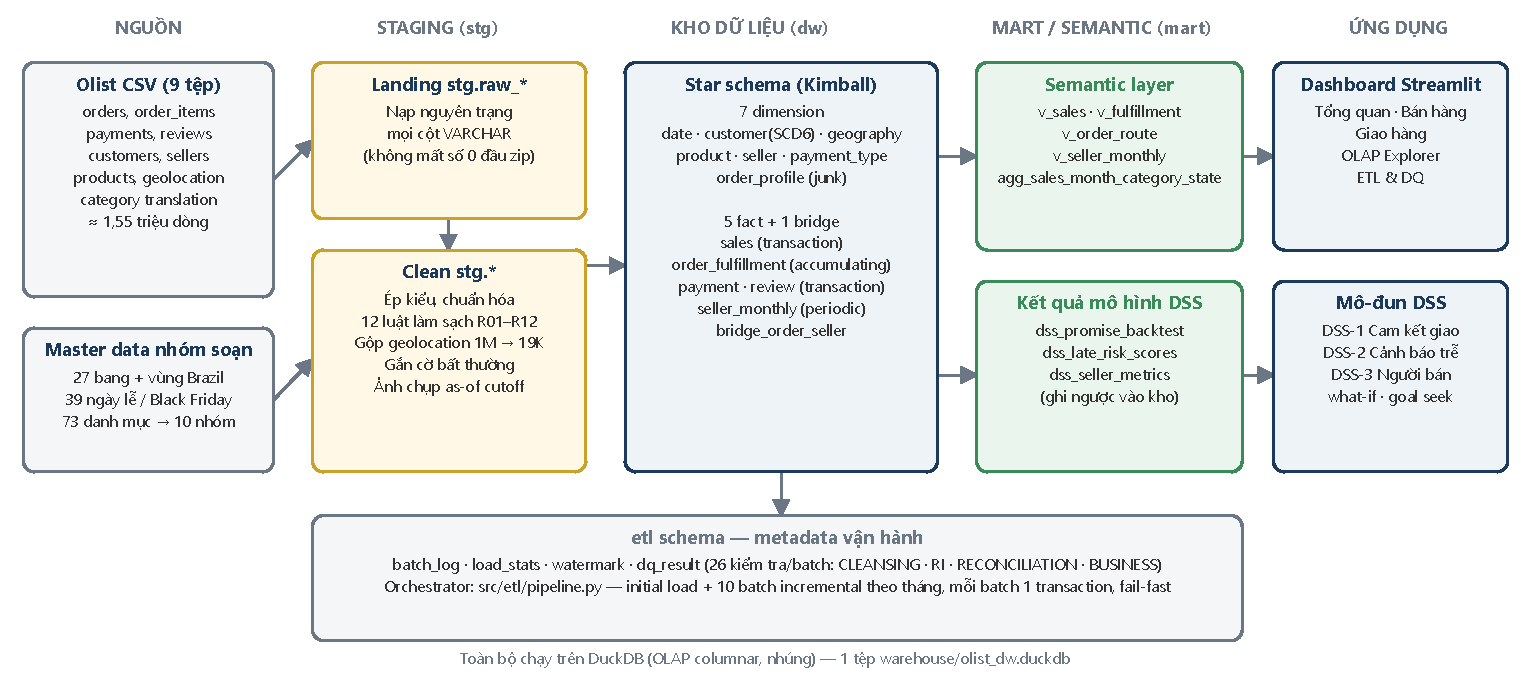
\includegraphics[width=\textwidth]{d_architecture.pdf}
    \caption{Kiến trúc hệ thống: nguồn $\rightarrow$ staging hai tầng $\rightarrow$ star schema $\rightarrow$ semantic layer $\rightarrow$ dashboard và DSS}
    \label{fig:arch}
\end{figure}

Hệ thống tuân theo kiến trúc nhiều tầng của Kimball (Hình~\ref{fig:arch}):
\begin{itemize}
    \item \textbf{Staging} (người dùng không truy cập) gồm hai tầng: tầng \textit{landing} lưu nguyên trạng, mọi cột ở dạng VARCHAR -- đảm bảo không mất thông tin và có thể kiểm tra lại (chính nhờ vậy phát hiện được lỗi mất số 0 của mã bưu chính); tầng \textit{clean} đã ép kiểu và chuẩn hóa.
    \item \textbf{dw}: lớp trình bày (presentation) dạng star schema.
    \item \textbf{mart}: lớp semantic gồm các view phẳng hóa và bảng tổng hợp; đồng thời là nơi các mô hình DSS \textbf{ghi ngược kết quả} vào kho.
    \item \textbf{etl}: metadata vận hành (nhật ký batch, watermark, kết quả kiểm tra chất lượng).
\end{itemize}
Hệ quản trị được chọn là \textbf{DuckDB}~\cite{duckdb2019} -- một engine OLAP lưu trữ theo cột, thực thi vector hóa, hỗ trợ đầy đủ \code{ROLLUP/CUBE/GROUPING SETS/PIVOT/QUALIFY} và chạy nhúng trong một tệp duy nhất, giúp tái lập toàn bộ hệ thống trên mọi máy (lý do chi tiết ở Mục~\ref{sec:decisions}).

\subsection{Quy trình thiết kế bốn bước của Kimball}
Với mỗi quy trình nghiệp vụ, nhóm áp dụng bốn bước: (1) chọn quy trình, (2) khai báo grain, (3) xác định dimension, (4) xác định fact (Bảng~\ref{tab:4step}).

\begin{table}[!htbp]
\centering
\caption{Kết quả áp dụng quy trình bốn bước của Kimball}
\label{tab:4step}
\small
\begin{tabularx}{\textwidth}{@{}>{\raggedright\arraybackslash}p{2.2cm} >{\raggedright\arraybackslash}p{2.6cm} l Y Y@{}}
\toprule
\thead{Quy trình} & \thead{Grain (1 dòng =)} & \thead{Loại fact} & \thead{Dimension} & \thead{Số đo} \\
\midrule
Bán hàng & 1 dòng sản phẩm của 1 đơn & Transaction & date ($\times$2), customer, product, seller, geography ($\times$2), order profile & quantity, price, freight, item total, distance \\
Thực hiện đơn & 1 đơn hàng, cập nhật qua các mốc & Accumulating & date ($\times$5), customer, geography, order profile & item count, order value, 6 độ trễ giữa các mốc, cờ trạng thái \\
Thanh toán & 1 lần thanh toán & Transaction & date, customer, payment type, order profile & installments, payment value \\
Đánh giá & 1 review & Transaction & date ($\times$3), customer & review score, is negative, response hours \\
Hiệu suất người bán & 1 người bán $\times$ 1 tháng & Periodic & date (cuối tháng), seller & orders, GMV, delivered, late, review, SLA, open orders \\
\bottomrule
\end{tabularx}
\end{table}

\textbf{Vì sao fact bán hàng có grain là dòng sản phẩm chứ không phải đơn hàng?} Grain nguyên tử nhất cho phép phân tích theo sản phẩm và người bán, vì một đơn có thể gồm nhiều sản phẩm từ nhiều người bán; các câu hỏi ở cấp đơn vẫn trả lời được bằng \code{COUNT(DISTINCT order_id)}. Ngược lại, quá trình giao hàng diễn ra ở cấp đơn nên fact thực hiện đơn có grain là đơn hàng. Tách hai fact theo hai grain khác nhau giúp tránh lỗi trộn grain và đếm trùng.

\subsection{Bus matrix}
\begin{table}[!htbp]
\centering
\caption{Bus matrix -- ``$\times n$'' là số vai trò (role-playing)}
\label{tab:bus}
\small
\resizebox{\textwidth}{!}{\begin{tabular}{@{}l c c c c c c c@{}}
\toprule
\thead{Quy trình \textbackslash\ Dimension} & \thead{Date} & \thead{Customer} & \thead{Geography} & \thead{Product} & \thead{Seller} & \thead{Profile} & \thead{Pay type} \\
\midrule
Bán hàng (\code{fact_sales}) & $\checkmark\times2$ & $\checkmark$ & $\checkmark\times2$ & $\checkmark$ & $\checkmark$ & $\checkmark$ & \\
Thực hiện đơn (\code{fact_order_fulfillment}) & $\checkmark\times5$ & $\checkmark$ & $\checkmark$ & & bridge & $\checkmark$ & \\
Thanh toán (\code{fact_payment}) & $\checkmark$ & $\checkmark$ & & & & $\checkmark$ & $\checkmark$ \\
Đánh giá (\code{fact_review}) & $\checkmark\times3$ & $\checkmark$ & & & bridge & & \\
Hiệu suất người bán (snapshot) & $\checkmark$ & & & & $\checkmark$ & & \\
\bottomrule
\end{tabular}}
\end{table}
Các dimension Date, Customer, Geography và Seller là \textbf{conformed dimension} dùng chung giữa các fact, cho phép thực hiện drill-across.

\subsection{Lược đồ dữ liệu}
Hình~\ref{fig:star-sales} trình bày star schema của quy trình bán hàng -- trung tâm của kho -- với sáu dimension, trong đó \code{dim_geography} đóng hai vai trò (nơi nhận và nơi gửi) và \code{dim_date} đóng hai vai trò (ngày đặt và hạn bàn giao). Hình~\ref{fig:star-fulfil} trình bày accumulating snapshot của quy trình thực hiện đơn: \code{dim_date} đóng năm vai trò ứng với năm mốc của đơn; bridge table nối đơn với người bán để phân bổ các số đo cấp đơn; fact đánh giá liên kết qua khóa \code{order_id} (drill-across); periodic snapshot người bán được dựng từ chính các fact trong kho.
\begin{figure}[!htbp]
    \centering
    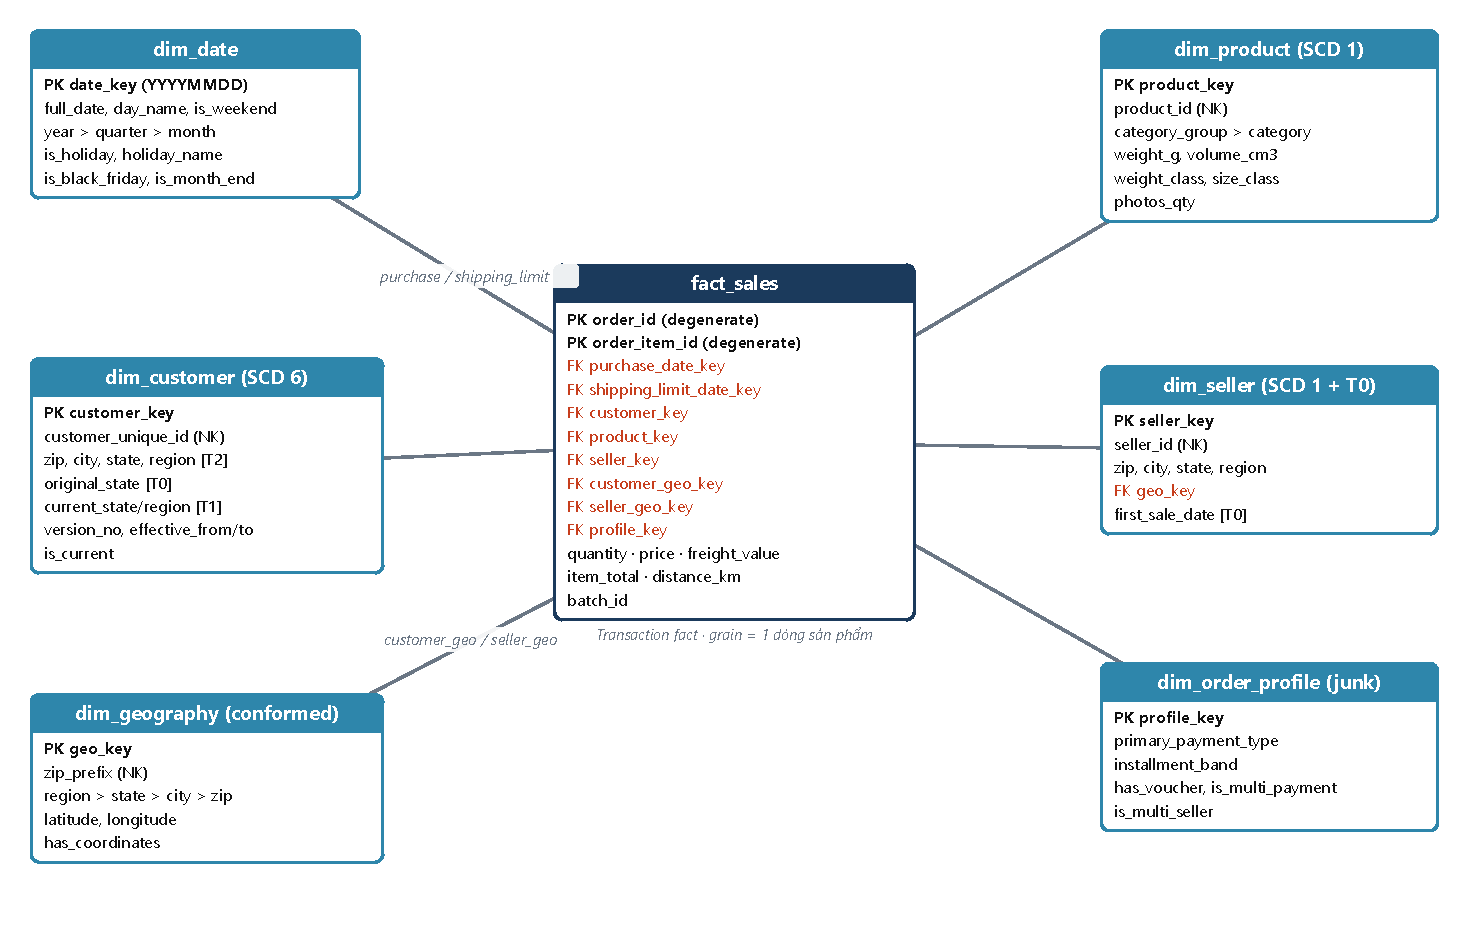
\includegraphics[width=\textwidth]{d_star_sales.pdf}
    \caption{Star schema của quy trình Bán hàng (màu đỏ: khóa ngoại; [T0]/[T1]/[T2]: kiểu SCD của thuộc tính)}
    \label{fig:star-sales}
\end{figure}

\begin{figure}[!htbp]
    \centering
    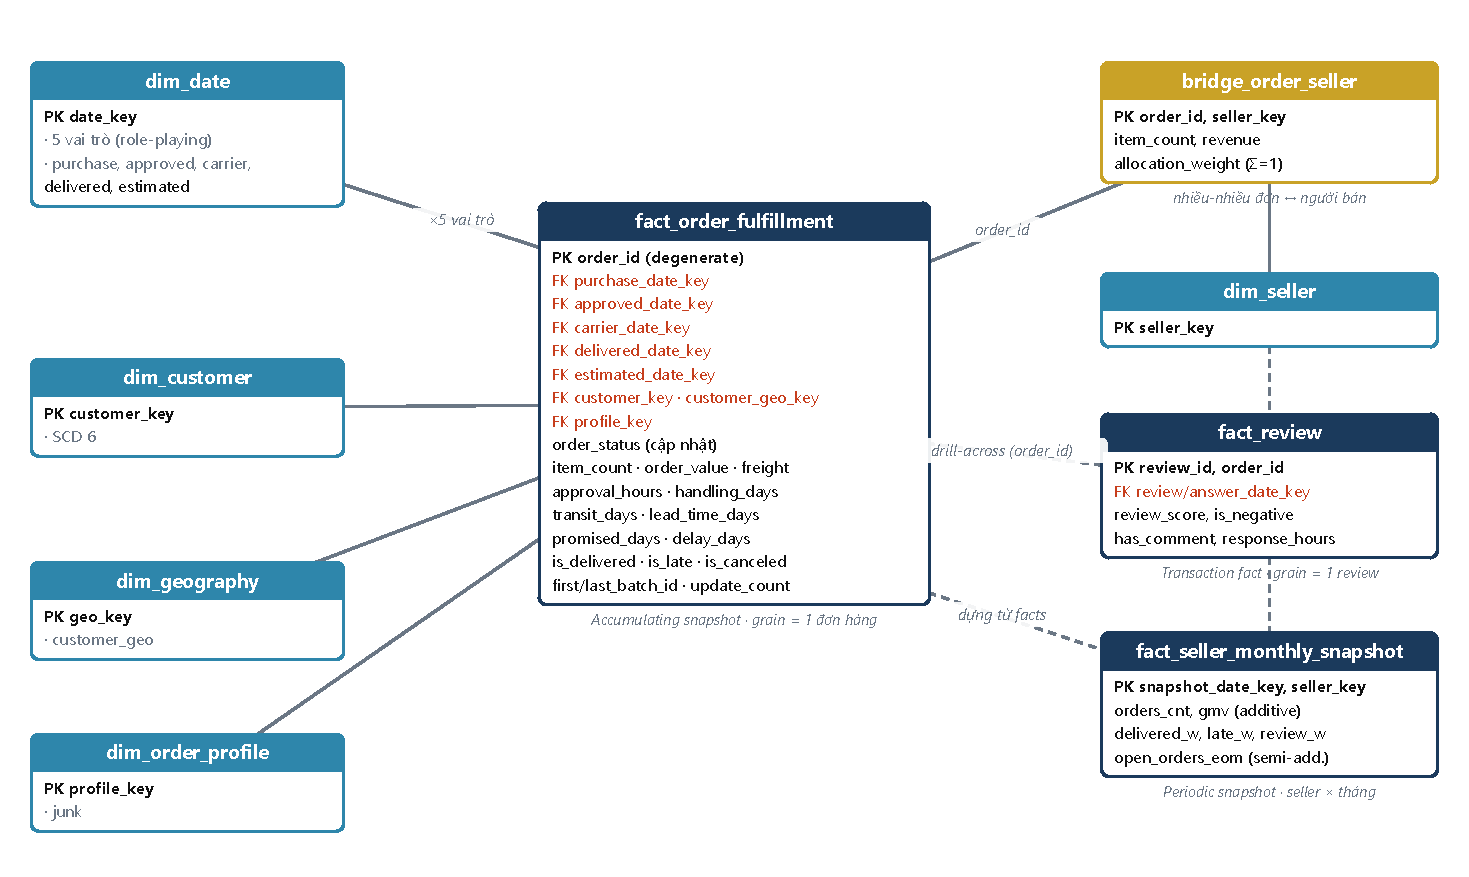
\includegraphics[width=\textwidth]{d_star_fulfillment.pdf}
    \caption{Accumulating snapshot Thực hiện đơn, bridge table và liên kết với fact đánh giá, periodic snapshot người bán}
    \label{fig:star-fulfil}
\end{figure}

\subsection{Đặc tả dimension}
\begin{table}[!htbp]
\centering
\caption{Đặc tả các dimension}
\label{tab:dims}
\small
\begin{tabularx}{\textwidth}{@{}l r Y Y@{}}
\toprule
\thead{Dimension} & \thead{Số dòng} & \thead{Thuộc tính chính / phân cấp} & \thead{Chiến lược thay đổi} \\
\midrule
\code{dim_date} & 1.828 & Ngày $\rightarrow$ tháng $\rightarrow$ quý $\rightarrow$ năm; thứ, cuối tuần, ngày lễ Brazil, Black Friday & Sinh sẵn 2016--2020; khóa YYYYMMDD; $-1$ = chưa xảy ra \\
\code{dim_customer} & 96.356 & Mã khách; zip, thành phố, bang, vùng; bang ban đầu; bang hiện tại & \textbf{SCD Type 6} = T2 (địa chỉ) + T1 (\code{current_*}) + T0 (\code{original_state}) \\
\code{dim_geography} & 19.180 & Vùng $\rightarrow$ bang $\rightarrow$ thành phố $\rightarrow$ zip; tọa độ & SCD1; conformed, role-playing \\
\code{dim_product} & 32.952 & Nhóm ngành $\rightarrow$ danh mục $\rightarrow$ sản phẩm; trọng lượng, thể tích, phân lớp kích thước & SCD1 \\
\code{dim_seller} & 3.096 & Mã người bán; địa chỉ; ngày bán đầu tiên & SCD1 + Type 0 (\code{first_sale_date}) \\
\code{dim_payment_type} & 5 & Loại thanh toán, nhãn tiếng Việt, \code{is_card} & Tĩnh \\
\code{dim_order_profile} & 161 & Phương thức chính, số kỳ trả góp, có voucher, nhiều lần trả, nhiều người bán & \textbf{Junk}: sinh sẵn $5\times4\times2\times2\times2 = 160$ tổ hợp \\
\bottomrule
\end{tabularx}
\end{table}

Mọi dimension đều dùng \textbf{surrogate key} (số nguyên sinh từ sequence), tách biệt với khóa tự nhiên của hệ nguồn. Đây là điều kiện bắt buộc để một khách hàng có thể có nhiều phiên bản (SCD2) và để fact không phụ thuộc vào hệ nguồn. Mỗi dimension có một thành viên đặc biệt mang khóa $-1$ (Unknown) để fact không bao giờ chứa khóa ngoại NULL.

\subsection{Đặc tả fact}
\begin{table}[!htbp]
\centering
\caption{Đặc tả các fact table và bridge table}
\label{tab:facts}
\small
\begin{tabularx}{\textwidth}{@{}l r Y Y@{}}
\toprule
\thead{Fact} & \thead{Số dòng} & \thead{Số đo additive} & \thead{Semi- / non-additive} \\
\midrule
\code{fact_sales} & 112.650 & quantity, price, freight value, item total & distance (AVG) \\
\code{fact_order_fulfillment} & 99.441 & item count, order value, freight, payment value & 6 độ trễ (AVG), cờ trạng thái (tỷ lệ) \\
\code{fact_payment} & 103.886 & payment value & installments (AVG) \\
\code{fact_review} & 99.224 & số review, số review tiêu cực & review score (AVG), response hours \\
\code{fact_seller_monthly_snapshot} & 39.678 & orders, GMV, delivered, late, review weight, review score sum, SLA breach & open orders, cumulative GMV (semi); số khách (distinct) \\
\code{bridge_order_seller} & 100.010 & \multicolumn{2}{p{7.6cm}}{\code{allocation_weight} = doanh thu của người bán trong đơn / doanh thu đơn; tổng trọng số mỗi đơn bằng 1} \\
\bottomrule
\end{tabularx}
\end{table}

Điểm đáng chú ý trong thiết kế periodic snapshot: thay vì lưu sẵn các tỷ lệ, bảng lưu \textbf{tử số và mẫu số} (ví dụ \code{review_score_sum_w} và \code{review_w}, \code{late_w} và \code{delivered_w}). Nhờ vậy các số đo vẫn cộng được qua nhiều tháng, nhiều người bán, và tỷ lệ chỉ được tính \textit{sau khi cộng}:
\begin{equation}
\text{TỷLệĐúngHạn}(S, T) = 1 - \frac{\sum_{s \in S}\sum_{t \in T} \text{late}_{s,t}}{\sum_{s \in S}\sum_{t \in T} \text{delivered}_{s,t}},
\end{equation}
tránh được lỗi kinh điển ``trung bình của trung bình''.

\subsection{Các kỹ thuật mô hình hóa nâng cao đã áp dụng}
\begin{table}[!htbp]
\centering
\caption{Tám kỹ thuật mô hình hóa nâng cao và căn cứ áp dụng}
\label{tab:techniques}
\small
\begin{tabularx}{\textwidth}{@{}>{\raggedright\arraybackslash}p{3.1cm} >{\raggedright\arraybackslash}p{4.2cm} Y@{}}
\toprule
\thead{Kỹ thuật} & \thead{Áp dụng ở đâu} & \thead{Căn cứ từ dữ liệu} \\
\midrule
SCD Type 2 $\rightarrow$ Type 6 & \code{dim_customer} & 250 khách dùng nhiều địa chỉ; doanh thu cần ghi nhận theo bang tại thời điểm mua (as-was), đồng thời cần phân tích theo địa chỉ hiện tại (as-is) \\
Ba loại fact & sales, payment, review; fulfillment; seller monthly & Sự kiện, tiến trình nhiều mốc và trạng thái định kỳ là ba câu hỏi khác nhau \\
Conformed dimension, bus matrix & Date, Customer, Geography, Seller & Drill-across doanh thu $\times$ trễ $\times$ hài lòng (Q08) \\
Degenerate dimension & \code{order_id}, \code{order_item_id} & Truy vết từng đơn; khóa để drill-across; không có thuộc tính mô tả riêng \\
Junk dimension & \code{dim_order_profile} & 5 cờ ít giá trị gom thành 1 khóa ngoại thay vì 5 cột \\
Role-playing dimension & Date $\times$5 (fulfillment), Geography $\times$2 (sales) & Đơn có 5 mốc thời gian; hàng đi từ nơi gửi tới nơi nhận (Q07) \\
Bridge table có trọng số & \code{bridge_order_seller} & Đánh giá và trễ hạn đo ở cấp đơn, nhưng đơn có thể có nhiều người bán \\
Aggregate table & \code{agg_sales_month_}\newline\code{category_state} & Tăng tốc dashboard 8,3 lần (Mục~\ref{sec:perf}) \\
\bottomrule
\end{tabularx}
\end{table}

\textbf{Mini-dimension} đã được cân nhắc cho phân khúc RFM của khách hàng (một thuộc tính thay đổi nhanh), nhưng không được áp dụng vì 96,9\% khách hàng chỉ mua một lần -- thuộc tính hành vi gần như không biến thiên, nên chi phí thêm một chiều không tương xứng với giá trị mang lại.

\subsection{Các quyết định thiết kế và phương án đã cân nhắc}
\label{sec:decisions}
\begin{itemize}
    \item \textbf{Star thay vì snowflake.} Phân cấp danh mục và địa lý được phi chuẩn hóa vào dimension. Các dimension đều nhỏ (\code{dim_product} khoảng 33 nghìn dòng) nên dư thừa không đáng kể, đổi lại truy vấn ít phép nối hơn và dễ hiểu hơn với người dùng nghiệp vụ.
    \item \textbf{Tách fact thanh toán khỏi fact bán hàng.} Thanh toán có grain riêng: một đơn có thể trả nhiều lần, nhiều phương thức, và tổng thanh toán lệch tổng đơn ở 312 đơn do lãi trả góp. Gộp vào fact bán hàng sẽ buộc phải phân bổ tùy tiện và gây đếm trùng.
    \item \textbf{Bridge thay vì gán ``người bán chính''.} Gán toàn bộ đánh giá cho một người bán chính sẽ sai với 1,3\% đơn có nhiều người bán; bridge có trọng số bảo toàn được tổng (kiểm tra RC05).
    \item \textbf{Periodic snapshot dạng dense.} Mọi người bán đã hoạt động đều có dòng ở mọi tháng, kể cả tháng không phát sinh đơn. Điều này giúp tính tăng trưởng, phát hiện người bán ngừng hoạt động và đơn giản hóa phép nối theo thời gian.
    \item \textbf{Snapshot được dựng từ các fact khác trong kho}, không đọc lại staging, bảo đảm một nguồn sự thật duy nhất; kiểm tra RC07 xác nhận tổng GMV khớp tuyệt đối.
    \item \textbf{Không khai báo FOREIGN KEY vật lý.} DuckDB không cho phép UPDATE dòng đang được tham chiếu, gây cản trở SCD1 và SCD6; nhiều kho dữ liệu thực tế cũng tắt khóa ngoại để tăng tốc nạp. Toàn vẹn tham chiếu được đảm bảo bằng các kiểm tra RI01--RI04 sau mỗi batch theo cơ chế fail-fast.
    \item \textbf{DuckDB thay vì PostgreSQL hoặc SQL Server.} Lưu trữ theo cột và thực thi vector hóa phù hợp với truy vấn phân tích; cú pháp OLAP đầy đủ; không cần máy chủ nên toàn bộ hệ thống có thể tái lập bằng một lệnh. Mã SQL tuân theo chuẩn ANSI, có thể chuyển sang PostgreSQL với chỉnh sửa nhỏ.
\end{itemize}

% ============================================================ 5
\section{Quy trình ETL}

\subsection{Tổng quan luồng xử lý}
\begin{figure}[!htbp]
    \centering
    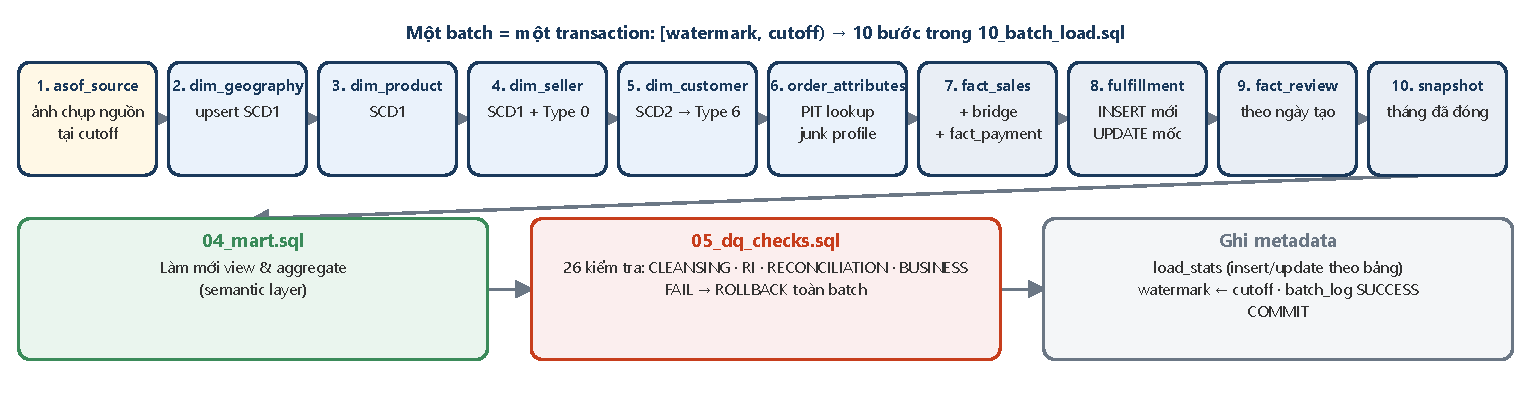
\includegraphics[width=\textwidth]{d_etl_flow.pdf}
    \caption{Luồng xử lý một batch ETL (\code{10_batch_load.sql}, điều phối bởi \code{pipeline.py})}
    \label{fig:etl}
\end{figure}

Pipeline gồm các script SQL thuần (đọc và chạy độc lập được), điều phối bởi \code{pipeline.py}:
\begin{enumerate}
    \item \code{01_staging.sql}: trích xuất và làm sạch;
    \item \code{02_dw_schema.sql}: định nghĩa lược đồ;
    \item \code{03_static_dims.sql}: sinh \code{dim_date}, junk dimension và các thành viên Unknown;
    \item \code{10_batch_load.sql}: biến đổi và nạp theo 10 bước, tách bởi marker \texttt{-{}-~@step} để đo thời gian từng bước (Hình~\ref{fig:etl});
    \item \code{04_mart.sql} và \code{05_dq_checks.sql}: làm mới lớp semantic và kiểm tra chất lượng.
\end{enumerate}
Mỗi batch chạy trong \textbf{một transaction}: nếu bất kỳ kiểm tra toàn vẹn hay đối soát nào thất bại, toàn bộ batch bị ROLLBACK và được ghi nhận là FAILED, nhờ đó kho không bao giờ rơi vào trạng thái nạp dở dang.

\subsection{Nạp tăng dần và mô phỏng hệ nguồn theo thời điểm}
Bộ dữ liệu Olist chỉ là ảnh chụp \textit{trạng thái cuối cùng}. Để ETL tăng dần và accumulating snapshot hoạt động như trong thực tế, nhóm xây dựng bước \code{asof_source}: với mốc cắt \textit{cutoff} của batch, mọi mốc thời gian sau cutoff được coi là \textit{chưa xảy ra} (gán NULL), và trạng thái đơn được suy diễn lại theo các mốc đã xảy ra. Ví dụ, đơn đã bàn giao vận chuyển nhưng chưa giao tại thời điểm cutoff có trạng thái \textit{shipped}. Kho được nạp bằng \textbf{1 batch khởi tạo} (mọi đơn trước 01/01/2018) và \textbf{10 batch tăng dần theo tháng} đến 01/11/2018; ranh giới các batch được quản lý bằng \textbf{watermark} lưu trong \code{etl.watermark}.

\begin{table}[!htbp]
\centering
\caption{Nhật ký thực thi các batch ETL (\code{etl.batch_log}, \code{etl.load_stats})}
\label{tab:batches}
\small
\resizebox{\textwidth}{!}{\begin{tabular}{@{}c l l r r r r r r@{}}
\toprule
\thead{Batch} & \thead{Loại} & \thead{Cửa sổ} & \thead{+Sales} & \thead{+Fulfil.} & \thead{UPD fulfil.} & \thead{SCD2} & \thead{+Snapshot} & \thead{Giây} \\
\midrule
1 & INITIAL & $\rightarrow$ 2018-01-01 & 51.234 & 45.430 & 0 & 0 & 13.548 & 1,5 \\
2 & INCR & 2018-01 & 8.208 & 7.269 & 2.456 & 24 & 1.952 & 1,0 \\
3 & INCR & 2018-02 & 7.672 & 6.728 & 2.853 & 7 & 2.072 & 1,2 \\
4 & INCR & 2018-03 & 8.217 & 7.211 & 3.465 & 25 & 2.185 & 1,1 \\
5 & INCR & 2018-04 & 7.975 & 6.939 & 3.698 & 15 & 2.387 & 1,3 \\
6 & INCR & 2018-05 & 7.925 & 6.873 & 2.741 & 21 & 2.559 & 1,3 \\
7 & INCR & 2018-06 & 7.078 & 6.167 & 2.423 & 17 & 2.750 & 1,4 \\
8 & INCR & 2018-07 & 7.092 & 6.292 & 1.687 & 18 & 2.940 & 1,5 \\
9 & INCR & 2018-08 & 7.248 & 6.512 & 2.010 & 18 & 3.095 & 2,0 \\
10 & INCR & 2018-09 & 1 & 16 & 56 & 0 & 3.095 & 1,4 \\
11 & INCR & 2018-10 & 0 & 4 & 3 & 0 & 3.095 & 1,3 \\
\bottomrule
\end{tabular}}
\end{table}

\begin{figure}[!htbp]
    \centering
    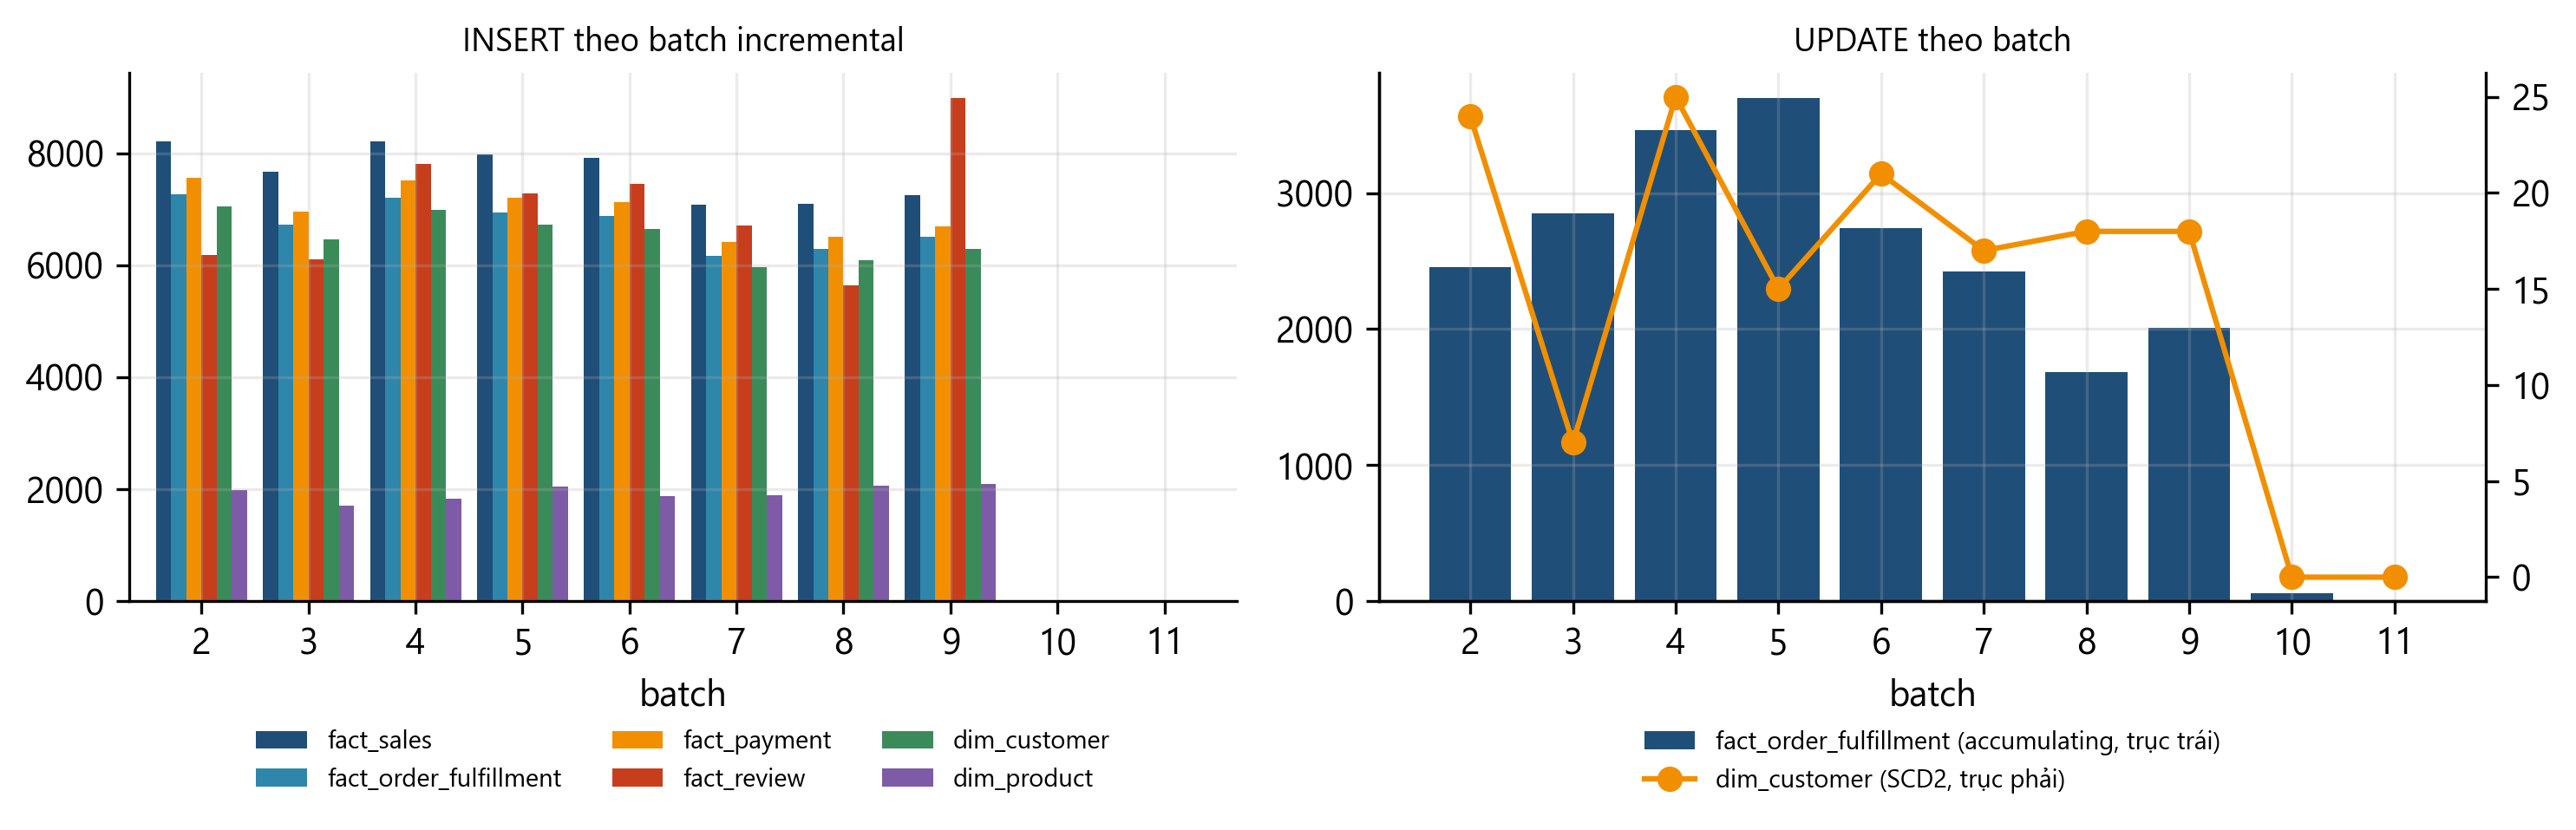
\includegraphics[width=\textwidth]{f7_etl.png}
    \caption{Số dòng INSERT và UPDATE theo batch: accumulating snapshot được cập nhật liên tục khi các đơn cũ đi qua mốc mới}
    \label{fig:etl-load}
\end{figure}

\subsection{Các luật làm sạch}
Các luật R01--R12 (Bảng~\ref{tab:dq}) được hiện thực bằng SQL khai báo ở tầng clean. Đoạn mã~\ref{lst:macro} minh họa hai macro chuẩn hóa dùng chung. Dữ liệu geolocation được gộp bằng median sau khi lọc các tọa độ nằm ngoài khung lãnh thổ ($\text{lat} \in [-34; 5{,}3]$, $\text{lng} \in [-74; -34]$); median được chọn vì bền vững với ngoại lai hơn trung bình cộng. Mỗi luật ghi số dòng bị ảnh hưởng vào \code{etl.dq_result} để có thể giải trình.

\begin{lstlisting}[caption={Macro chuẩn hóa tên thành phố và mã bưu chính (01\_staging.sql)}, label={lst:macro}]
CREATE OR REPLACE MACRO stg.norm_city(s) AS
    regexp_replace(lower(trim(strip_accents(s))), '\s+', ' ', 'g');
CREATE OR REPLACE MACRO stg.norm_zip(z) AS lpad(trim(z), 5, '0');
\end{lstlisting}

\subsection{Thuật toán SCD Type 2/6 cho dimension khách hàng}
Mỗi đơn hàng mang một địa chỉ giao hàng của khách (định danh bởi \code{customer_unique_id}). Thuật toán~\ref{alg:scd} được thực thi trong mỗi batch, hoàn toàn bằng SQL với hàm cửa sổ \code{LAG}/\code{LEAD}.

\begin{algorithm}[H]
\caption{Cập nhật SCD Type 2/6 cho \code{dim_customer} trong một batch}
\label{alg:scd}
\KwIn{Các đơn mới trong cửa sổ $[\text{watermark}, \text{cutoff})$; \code{dim_customer} hiện tại}
\KwOut{\code{dim_customer} đã cập nhật}
$E \leftarrow$ chuỗi sự kiện (khách, thời điểm, zip, thành phố, bang) của các đơn mới\;
$E \leftarrow E \;\cup$ phiên bản hiện hành của các khách có trong $E$ (làm ``hạt giống'')\;
Sắp xếp $E$ theo (khách, thời điểm); dùng \code{LAG} so sánh địa chỉ với sự kiện liền trước\;
$C \leftarrow$ các sự kiện mới có địa chỉ \textbf{khác} sự kiện liền trước\;
\ForEach{khách $u$ có sự kiện trong $C$}{
    Đóng phiên bản hiện hành: \code{effective_to} $\leftarrow \min_{c \in C_u} t_c$, \code{is_current} $\leftarrow$ false\;
    Thêm các phiên bản mới với \code{version_no} tăng dần, \code{effective_to} $\leftarrow$ \code{LEAD}$(t)$ hoặc 9999-12-31\;
    \lIf{$u$ là khách mới}{phiên bản đầu có \code{effective_from} = 1900-01-01}
}
\textbf{Type 1:} ghi đè \code{current_state} và \code{current_region} trên \textit{mọi} phiên bản của $u$\;
\textbf{Type 0:} giữ nguyên \code{original_state} từ lần xuất hiện đầu tiên\;
\end{algorithm}

Khi nạp fact, khóa khách hàng được tra cứu theo nguyên tắc \textbf{point-in-time}:
\begin{equation}
\text{customer\_key}(o) = k \;\text{ sao cho }\; \text{effective\_from}_k \le \text{purchase\_ts}_o < \text{effective\_to}_k .
\end{equation}
Kết quả: 96.355 dòng cho 96.096 khách hàng, gồm \textbf{259 phiên bản mới} của 252 khách; 39 khách đã chuyển sang bang khác. Bảng~\ref{tab:scd-example} là một ví dụ thực tế trong kho.

\begin{table}[!htbp]
\centering
\caption{Ví dụ SCD Type 6: khách hàng chuyển từ Paraná (PR) sang Santa Catarina (SC)}
\label{tab:scd-example}
\small
\resizebox{\textwidth}{!}{\begin{tabular}{@{}c l l c c c l l c@{}}
\toprule
\thead{Ver.} & \thead{Zip} & \thead{Thành phố} & \thead{Bang} & \thead{Original} & \thead{Current} & \thead{Effective from} & \thead{Effective to} & \thead{Current?} \\
\midrule
1 & 82510 & curitiba & PR & PR & SC & 1900-01-01 & 2018-01-13 13:52 & false \\
2 & 88780 & imbituba & SC & PR & SC & 2018-01-13 13:52 & 9999-12-31 & true \\
\bottomrule
\end{tabular}}
\end{table}
Nhờ vậy các đơn cũ vẫn được ghi nhận cho PR (as-was), đồng thời vẫn có thể phân tích theo SC (as-is).

\subsection{Cập nhật accumulating snapshot}
Với mọi đơn có thời điểm đặt trước cutoff, ETL tính lại trạng thái và các độ trễ tại thời điểm cutoff, sau đó so sánh với fact hiện có theo bộ (trạng thái, thời điểm duyệt, thời điểm bàn giao, thời điểm giao). Đơn mới được INSERT; đơn có mốc mới được UPDATE (khóa ngày của mốc, độ trễ, cờ trạng thái), đồng thời tăng \code{update_count} và ghi \code{last_batch_id}. Sau 10 batch tăng dần, 78.382 đơn chỉ nạp một lần, \textbf{20.726 đơn được cập nhật một lần và 333 đơn được cập nhật hai lần} (tổng cộng 21.392 thao tác UPDATE). Trạng thái cuối cùng khớp \textbf{100\%} với nguồn, được kiểm chứng bằng kiểm thử tự động.

\subsection{Kiểm soát chất lượng và đối soát}
Sau mỗi batch, hệ thống chạy 26 kiểm tra thuộc bốn nhóm. Kết quả của batch cuối cùng được tóm tắt trong Bảng~\ref{tab:dqres}.

\begin{table}[!htbp]
\centering
\caption{Kết quả kiểm tra chất lượng dữ liệu của batch cuối}
\label{tab:dqres}
\small
\begin{tabularx}{\textwidth}{@{}l Y r l@{}}
\toprule
\thead{Nhóm} & \thead{Kiểm tra} & \thead{Lỗi} & \thead{Kết quả} \\
\midrule
RI & RI01--RI03: mọi khóa ngoại của 5 fact và bridge tồn tại trong dimension (kể cả 5 vai trò của date); RI04: fact trỏ tới thành viên Unknown & 0 & PASS \\
Đối soát & RC01 số dòng fact bán hàng; RC02 tổng doanh thu (chính xác tới cent); RC03 số đơn; RC04 tổng thanh toán; RC05 tổng trọng số bridge bằng 1; RC06 SCD2 có đúng một phiên bản hiện hành và khoảng hiệu lực liên tục; RC07 GMV snapshot bằng GMV fact & 0 & PASS \\
Nghiệp vụ & BR01 điểm đánh giá thuộc $[1, 5]$; BR02 không có giá hoặc phí âm & 0 & PASS \\
Nghiệp vụ & BR03 tổng thanh toán lệch tổng đơn quá 1 BRL (do lãi trả góp) & 312 & FLAGGED \\
Làm sạch & R01--R12 (Bảng~\ref{tab:dq}) & -- & FIXED / FLAGGED \\
\bottomrule
\end{tabularx}
\end{table}

% ============================================================ 6
\section{OLAP và Dashboard}

\subsection{Lớp semantic}
Lớp \code{mart} che giấu độ phức tạp của star schema khỏi người dùng cuối:
\begin{itemize}
    \item \code{v_sales}: fact bán hàng đã được nối đủ sáu chiều;
    \item \code{v_fulfillment}: bổ sung phân nhóm mức trễ và đánh giá mới nhất của đơn;
    \item \code{v_order_route}: drill-across giữa fact thực hiện đơn, bridge và fact bán hàng để có tuyến nơi gửi $\rightarrow$ nơi nhận;
    \item \code{v_seller_monthly}: tính các tỷ lệ từ tử số và mẫu số của snapshot;
    \item \code{agg_sales_month_category_state}: bảng tổng hợp vật lý (11.823 dòng).
\end{itemize}

\subsection{Bộ truy vấn OLAP}
Tệp \code{olap_queries.sql} chứa 14 truy vấn; mỗi truy vấn gắn với một phép OLAP và một câu hỏi nghiệp vụ cụ thể (Bảng~\ref{tab:olap}). Trang OLAP Explorer của dashboard đọc trực tiếp từ tệp này.

\begin{table}[!htbp]
\centering
\caption{Bộ 14 truy vấn OLAP và thời gian thực thi}
\label{tab:olap}
\small
\begin{tabularx}{\textwidth}{@{}l l Y r@{}}
\toprule
\thead{Mã} & \thead{Phép OLAP} & \thead{Câu hỏi nghiệp vụ} & \thead{ms} \\
\midrule
Q01 & Roll-up (ROLLUP) & Doanh thu theo năm $\rightarrow$ quý $\rightarrow$ tháng, kèm tổng phụ & 86 \\
Q02 & Drill-down & Nhóm Electronics \& Tech $\rightarrow$ từng danh mục con & 16 \\
Q03 & Slice & Năm 2018: doanh thu, AOV, \% phí vận chuyển theo vùng & 17 \\
Q04 & Dice & H1-2018 $\times$ Sudeste $\times$ \{Health \& Beauty, Fashion\} $\times$ thẻ tín dụng & 16 \\
Q05 & Pivot & Nhóm ngành (hàng) $\times$ năm (cột) & 30 \\
Q06 & CUBE & Mọi tổ hợp vùng $\times$ phương thức thanh toán, có \code{GROUPING()} & 93 \\
Q07 & Grouping sets + role-playing & Luồng hàng vùng người bán $\rightarrow$ vùng khách hàng & 16 \\
Q08 & Drill-across & Doanh thu $\times$ \% trễ $\times$ điểm đánh giá theo nhóm ngành (3 fact) & 43 \\
Q09 & Ranking & Top-3 danh mục mỗi vùng (\code{QUALIFY}) & 15 \\
Q10 & Chuỗi thời gian & Trung bình trượt 3 tháng, tăng trưởng MoM và YoY & 9 \\
Q11 & SCD Type 6 & Doanh thu as-was và as-is của khách đã chuyển bang & 38 \\
Q12 & Semi-additive & Tồn đơn cuối kỳ: cộng theo tháng (sai) và trung bình/cuối kỳ (đúng) & 8 \\
Q13 & Accumulating (lag) & Phân rã chu trình đơn theo quý & 12 \\
Q14 & Aggregate navigation & Câu hỏi quý $\times$ vùng $\times$ ngành trên bảng tổng hợp & 6 \\
\bottomrule
\end{tabularx}
\end{table}

Đoạn mã~\ref{lst:rollup} minh họa truy vấn Q01; các dòng tổng theo năm và tổng toàn bộ được \code{ROLLUP} sinh tự động.

\begin{lstlisting}[caption={Truy vấn Q01 -- Roll-up doanh thu theo phân cấp thời gian}, label={lst:rollup}]
SELECT d.year_num, d.year_quarter, d.year_month,
       count(DISTINCT f.order_id) AS orders,
       round(sum(f.price), 0)     AS revenue
FROM dw.fact_sales f
JOIN dw.dim_date d ON d.date_key = f.purchase_date_key
WHERE d.year_num IN (2017, 2018)
GROUP BY ROLLUP (d.year_num, d.year_quarter, d.year_month)
ORDER BY 1 NULLS LAST, 2 NULLS LAST, 3 NULLS LAST;
\end{lstlisting}

Kết quả Q12 cho thấy tầm quan trọng của tính semi-additive: với quý 2018-Q1, nếu cộng tồn đơn của ba tháng ta được 14.170 -- một con số vô nghĩa -- trong khi tồn đơn trung bình cuối tháng là 4.723 và tồn đơn cuối quý là 5.217, trùng khớp với đỉnh tắc nghẽn quan sát được ở Q13. Kết quả Q11 cho thấy với 39 khách đã chuyển bang, doanh thu của bang São Paulo theo địa chỉ hiện tại cao hơn 2.069 BRL so với khi ghi nhận theo thời điểm mua -- minh chứng rằng hai góc nhìn as-was và as-is cho kết quả khác nhau và đều cần thiết.

\subsection{Hiệu năng và aggregate navigation}
\label{sec:perf}
Với cùng câu hỏi ``số đơn và doanh thu năm 2018 theo quý $\times$ vùng $\times$ nhóm ngành'', truy vấn trên fact chi tiết (112.650 dòng, 3 phép nối) mất \textbf{30,5 ms}; trên bảng tổng hợp (11.823 dòng, không phép nối) chỉ mất \textbf{3,7 ms} -- nhanh hơn \textbf{8,3 lần} (trung vị của 15 lần chạy). Toàn bộ truy vấn OLAP đều hoàn tất dưới 100 ms (trung vị của 5 lần chạy), đủ đáp ứng tương tác thời gian thực. Lưu ý rằng số đơn trong bảng tổng hợp chỉ là xấp xỉ khi cộng qua các danh mục (một đơn có nhiều danh mục sẽ bị đếm nhiều lần); đánh đổi này được chú thích rõ trên dashboard.

\subsection{Dashboard}
Dashboard được xây dựng bằng Streamlit với 8 trang chia thành ba nhóm: \textit{Phân tích} (Tổng quan, Bán hàng, Giao hàng, OLAP Explorer), \textit{Hỗ trợ quyết định} (3 mô-đun DSS) và \textit{Vận hành} (ETL và chất lượng dữ liệu). Trang \textbf{OLAP Explorer} cho phép người dùng tự chọn chiều hàng và chiều cột, kéo thanh trượt để roll-up hoặc drill-down theo phân cấp, lọc để slice/dice, xoay pivot, bật/tắt dòng tổng ROLLUP, và luôn hiển thị câu lệnh SQL được sinh ra.

\begin{figure}[!htbp]
    \centering
    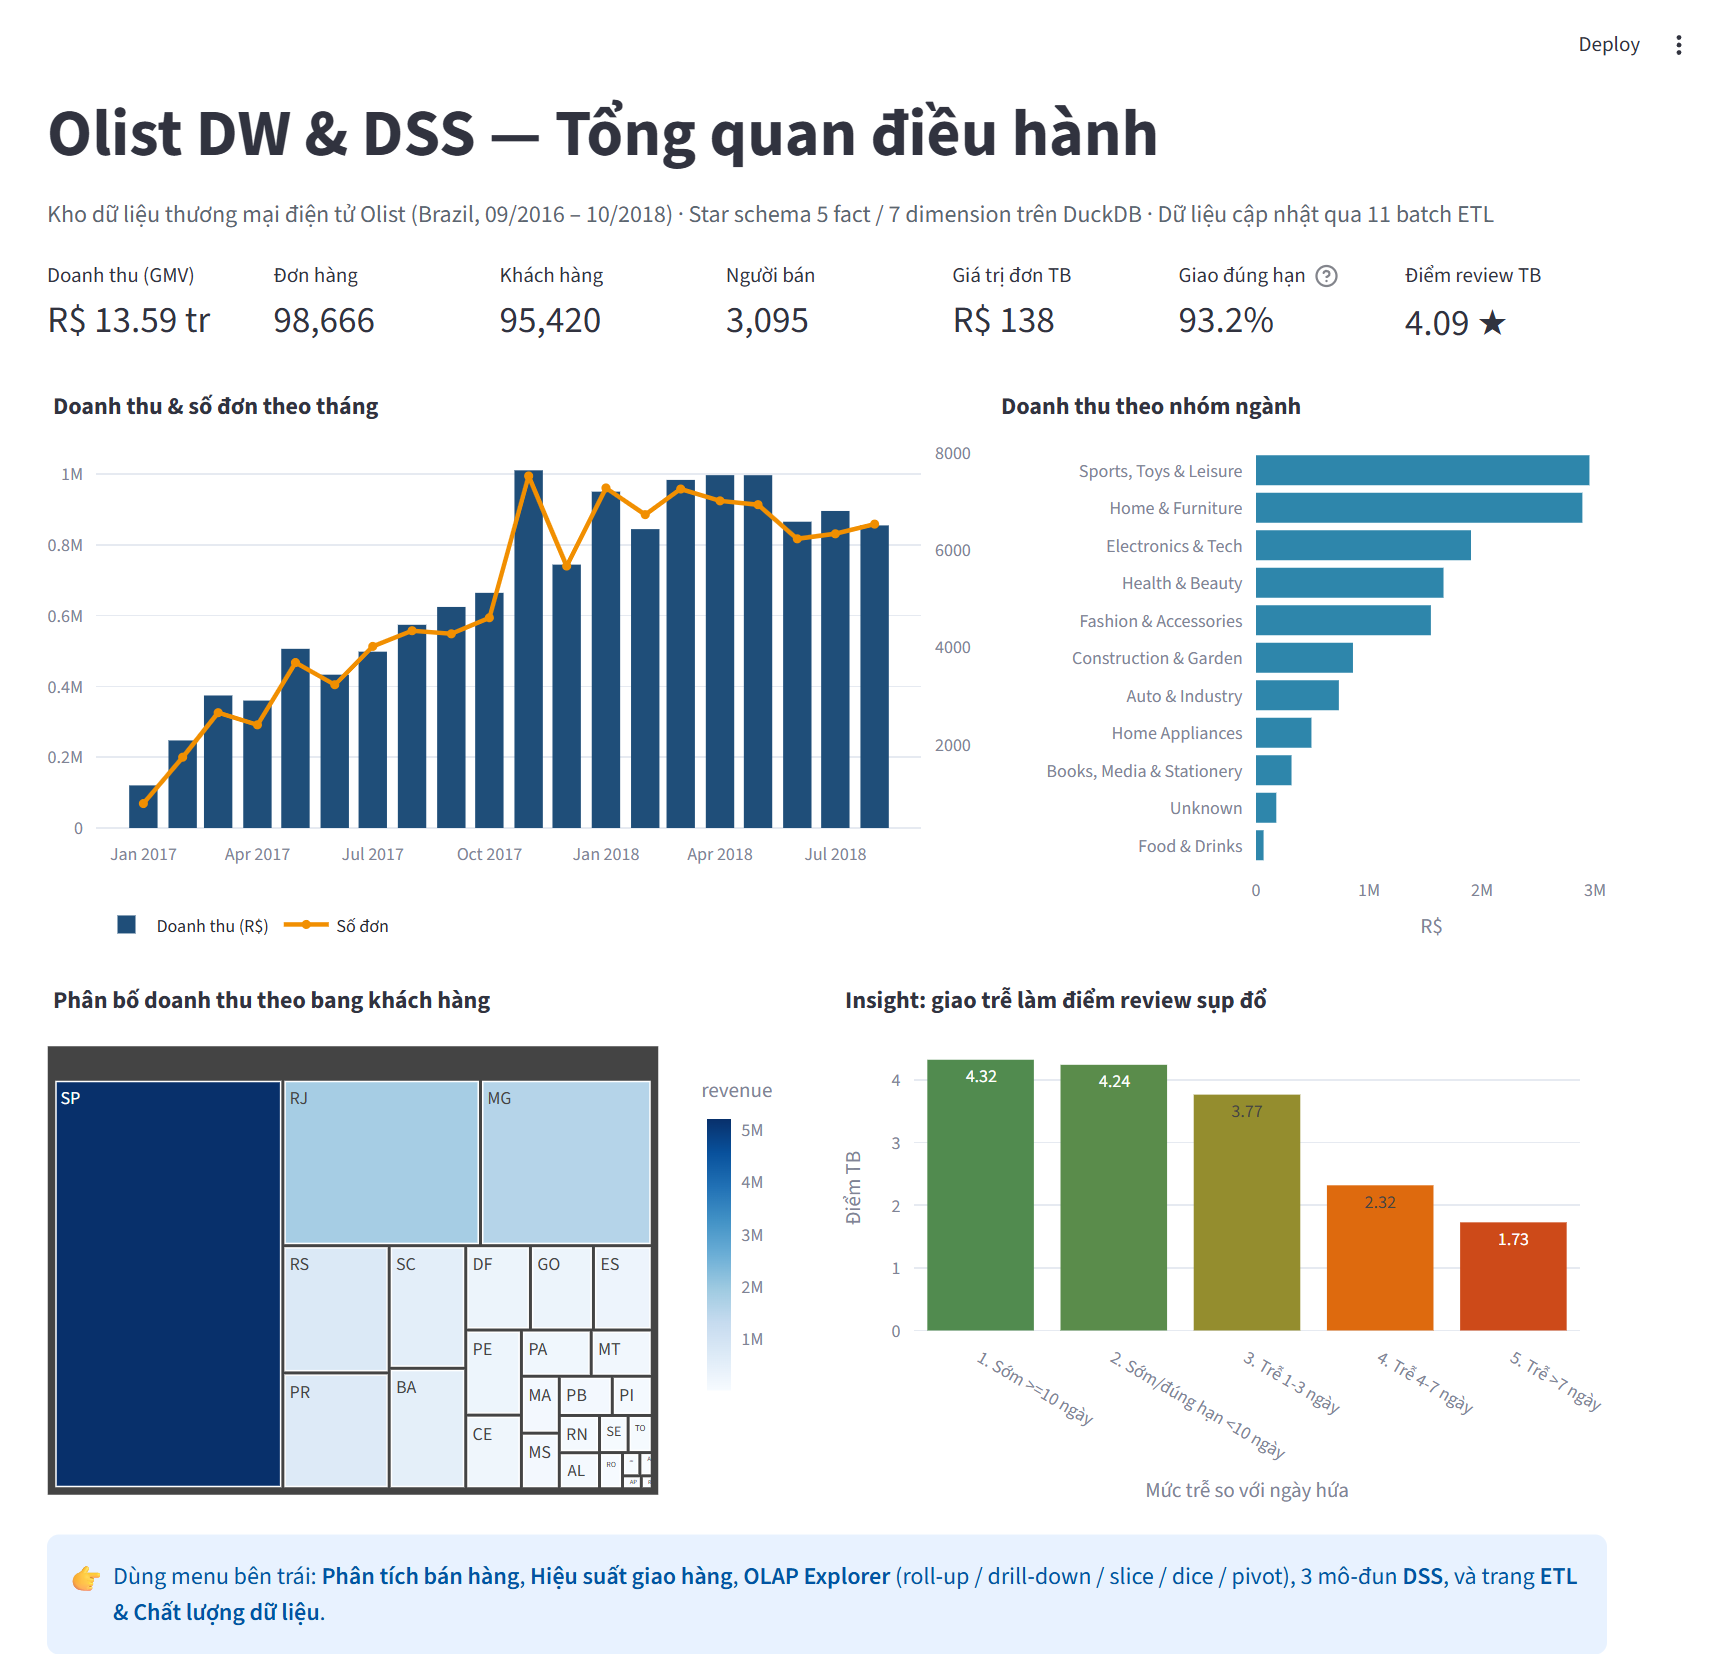
\includegraphics[width=0.95\textwidth]{home_c.png}
    \caption{Trang Tổng quan điều hành của dashboard}
    \label{fig:dash-home}
\end{figure}

\begin{figure}[!htbp]
    \centering
    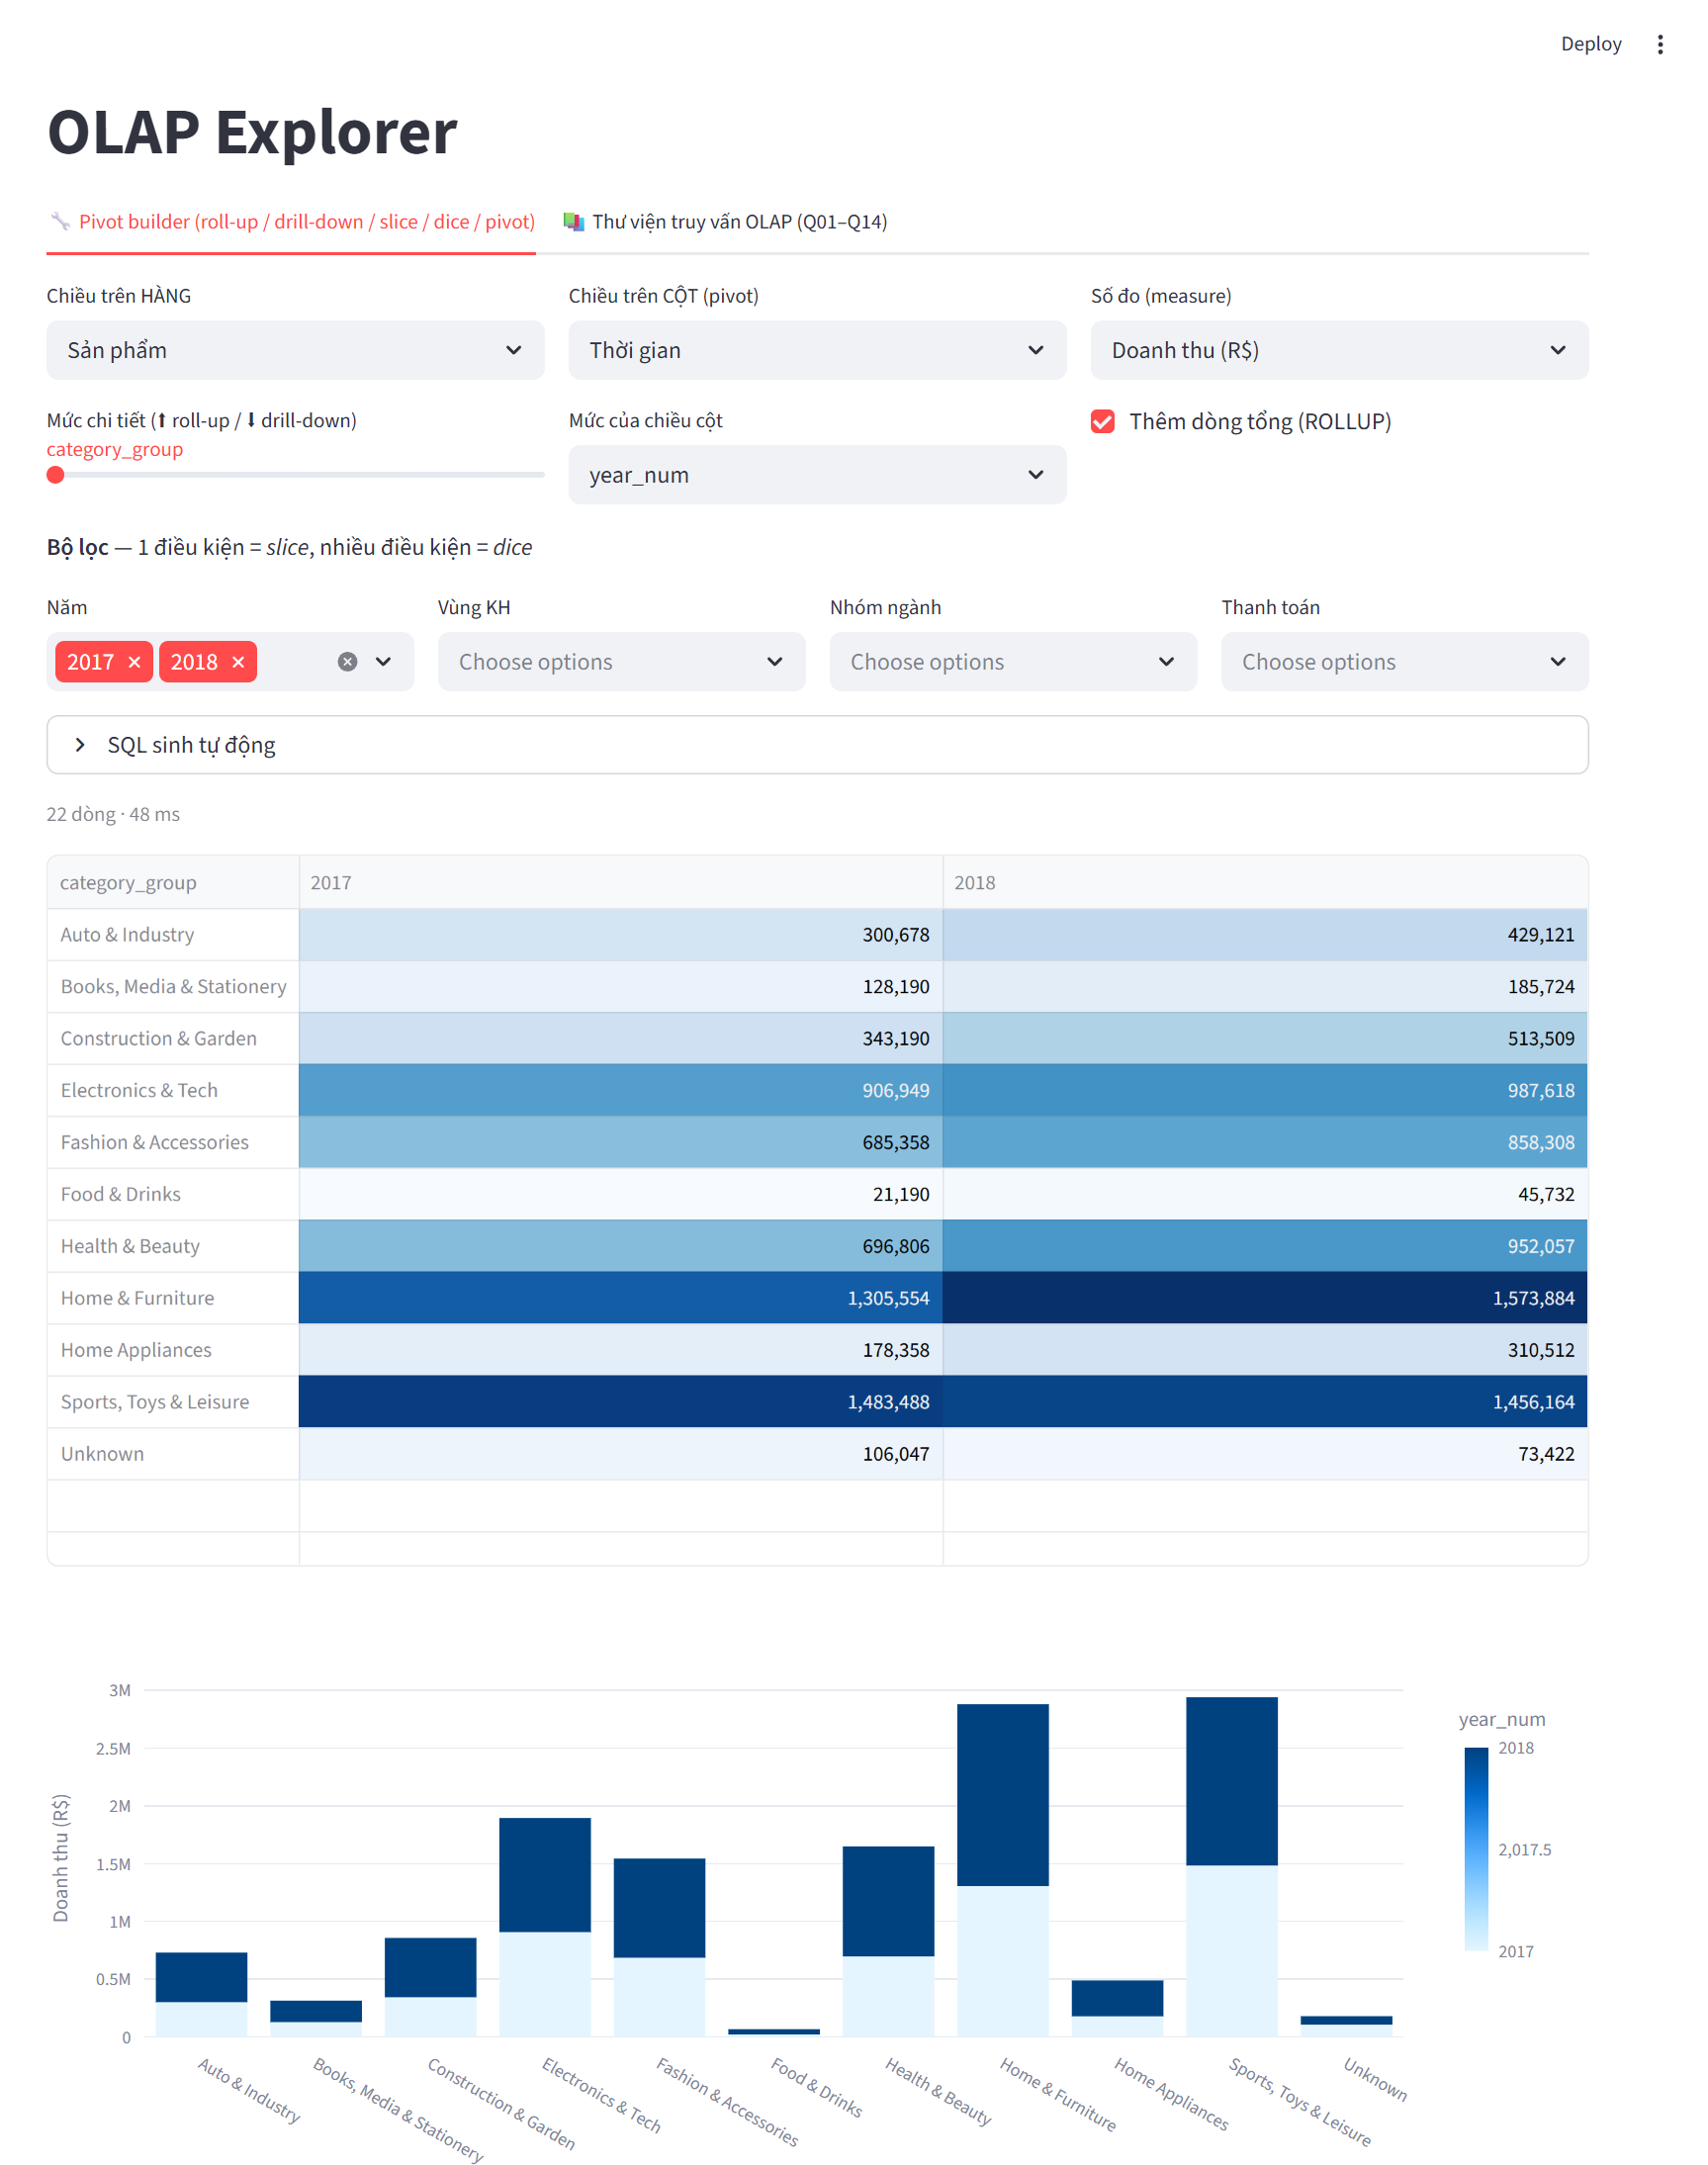
\includegraphics[width=0.95\textwidth,trim=0 545 0 0,clip]{olap_c.png}
    \caption{OLAP Explorer: pivot nhóm ngành $\times$ năm, drill-down và SQL sinh tự động}
    \label{fig:dash-olap}
\end{figure}

\subsection{Các phát hiện phân tích chính}
\begin{figure}[!htbp]
    \centering
    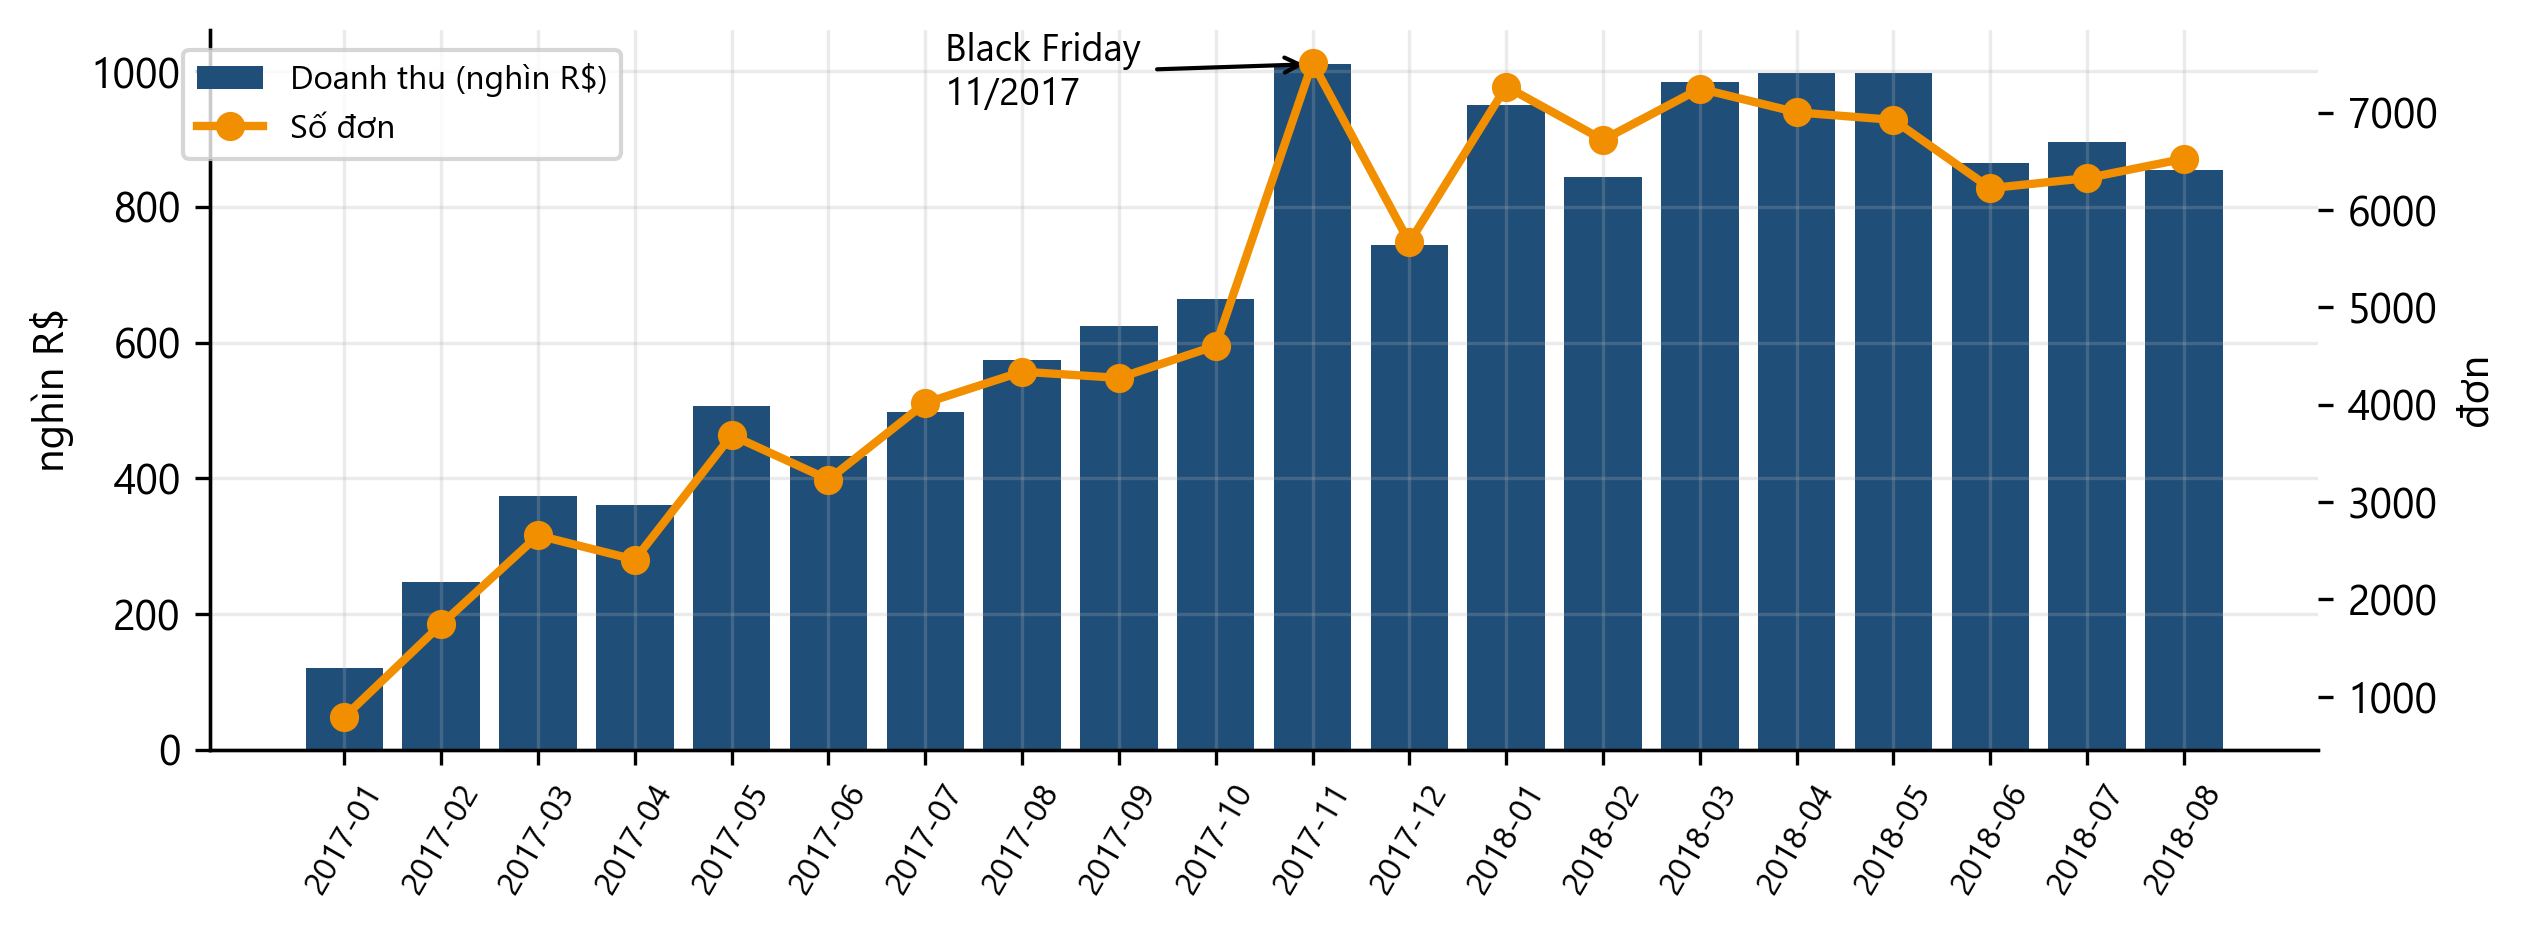
\includegraphics[width=0.9\textwidth]{f1_monthly.png}
    \caption{Doanh thu và số đơn theo tháng (01/2017--08/2018)}
    \label{fig:monthly}
\end{figure}

\begin{itemize}
    \item \textbf{Tăng trưởng và mùa vụ:} GMV tăng từ khoảng 120 nghìn BRL (01/2017) lên xấp xỉ 1 triệu BRL mỗi tháng; đỉnh rơi vào 11/2017 (Black Friday, tăng 52\% so với tháng trước) (Hình~\ref{fig:monthly}). Dù năm 2018 chỉ có 8 tháng dữ liệu, 9/10 nhóm ngành (trừ Sports, Toys \& Leisure) đã vượt doanh thu của cả năm 2017; tăng mạnh nhất là Food \& Drinks (+116\%, quy mô nhỏ), Home Appliances (+74\%) và Construction \& Garden (+50\%) (Q05).
    \item \textbf{Thị trường tập trung:} vùng Sudeste chiếm 66\% doanh thu năm 2018, nhưng các vùng xa (Norte, Nordeste) có AOV cao hơn và tỷ lệ phí vận chuyển trên doanh thu gấp khoảng 1,5 lần (23,9\% so với 15,5\%, Q03).
    \item \textbf{Cam kết dài nhưng vẫn trễ khi có cú sốc:} số ngày cam kết trung bình là \textbf{23,7 ngày} trong khi thực tế chỉ \textbf{12,6 ngày} (người bán xử lý 2,8 ngày, vận chuyển 9,3 ngày). Tỷ lệ trễ chung là 6,8\% nhưng tăng vọt lên 12,9\% ở quý 2018-Q1 do thời gian vận chuyển kéo dài trong khi số ngày cam kết không đổi (Hình~\ref{fig:lag}).
    \item \textbf{Giao trễ làm sụt giảm mạnh mức độ hài lòng:} giao sớm hoặc đúng hạn đạt 4,24--4,32 điểm; trễ 4--7 ngày còn 2,32 điểm (61\% đánh giá tiêu cực); trễ trên 7 ngày chỉ còn \textbf{1,73 điểm (78\% tiêu cực)} (Hình~\ref{fig:review}). Với tỷ lệ khách quay lại dưới 1\% mỗi tháng, đánh giá tiêu cực là rủi ro lớn đối với một marketplace.
\end{itemize}

\begin{figure}[!htbp]
    \centering
    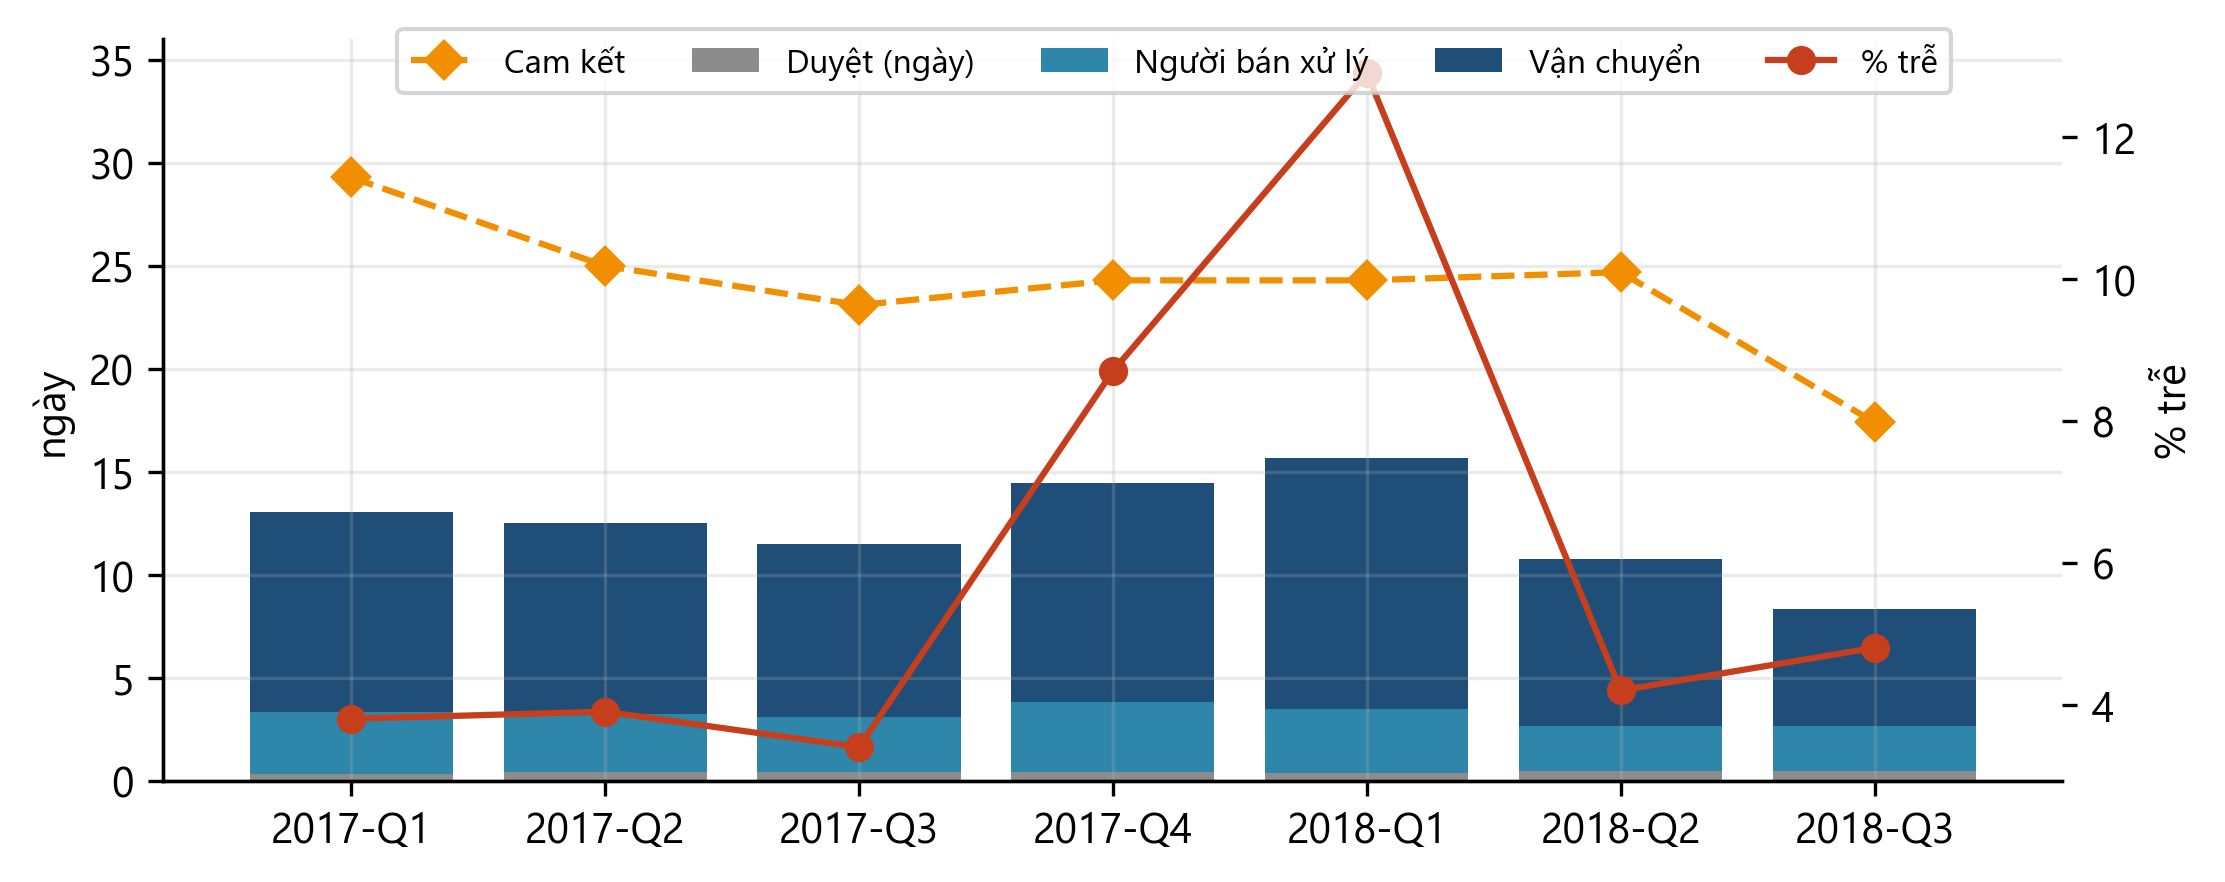
\includegraphics[width=0.85\textwidth]{f3_lag.png}
    \caption{Phân rã chu trình đơn hàng (accumulating snapshot) và tỷ lệ trễ theo quý}
    \label{fig:lag}
\end{figure}

\begin{figure}[!htbp]
    \centering
    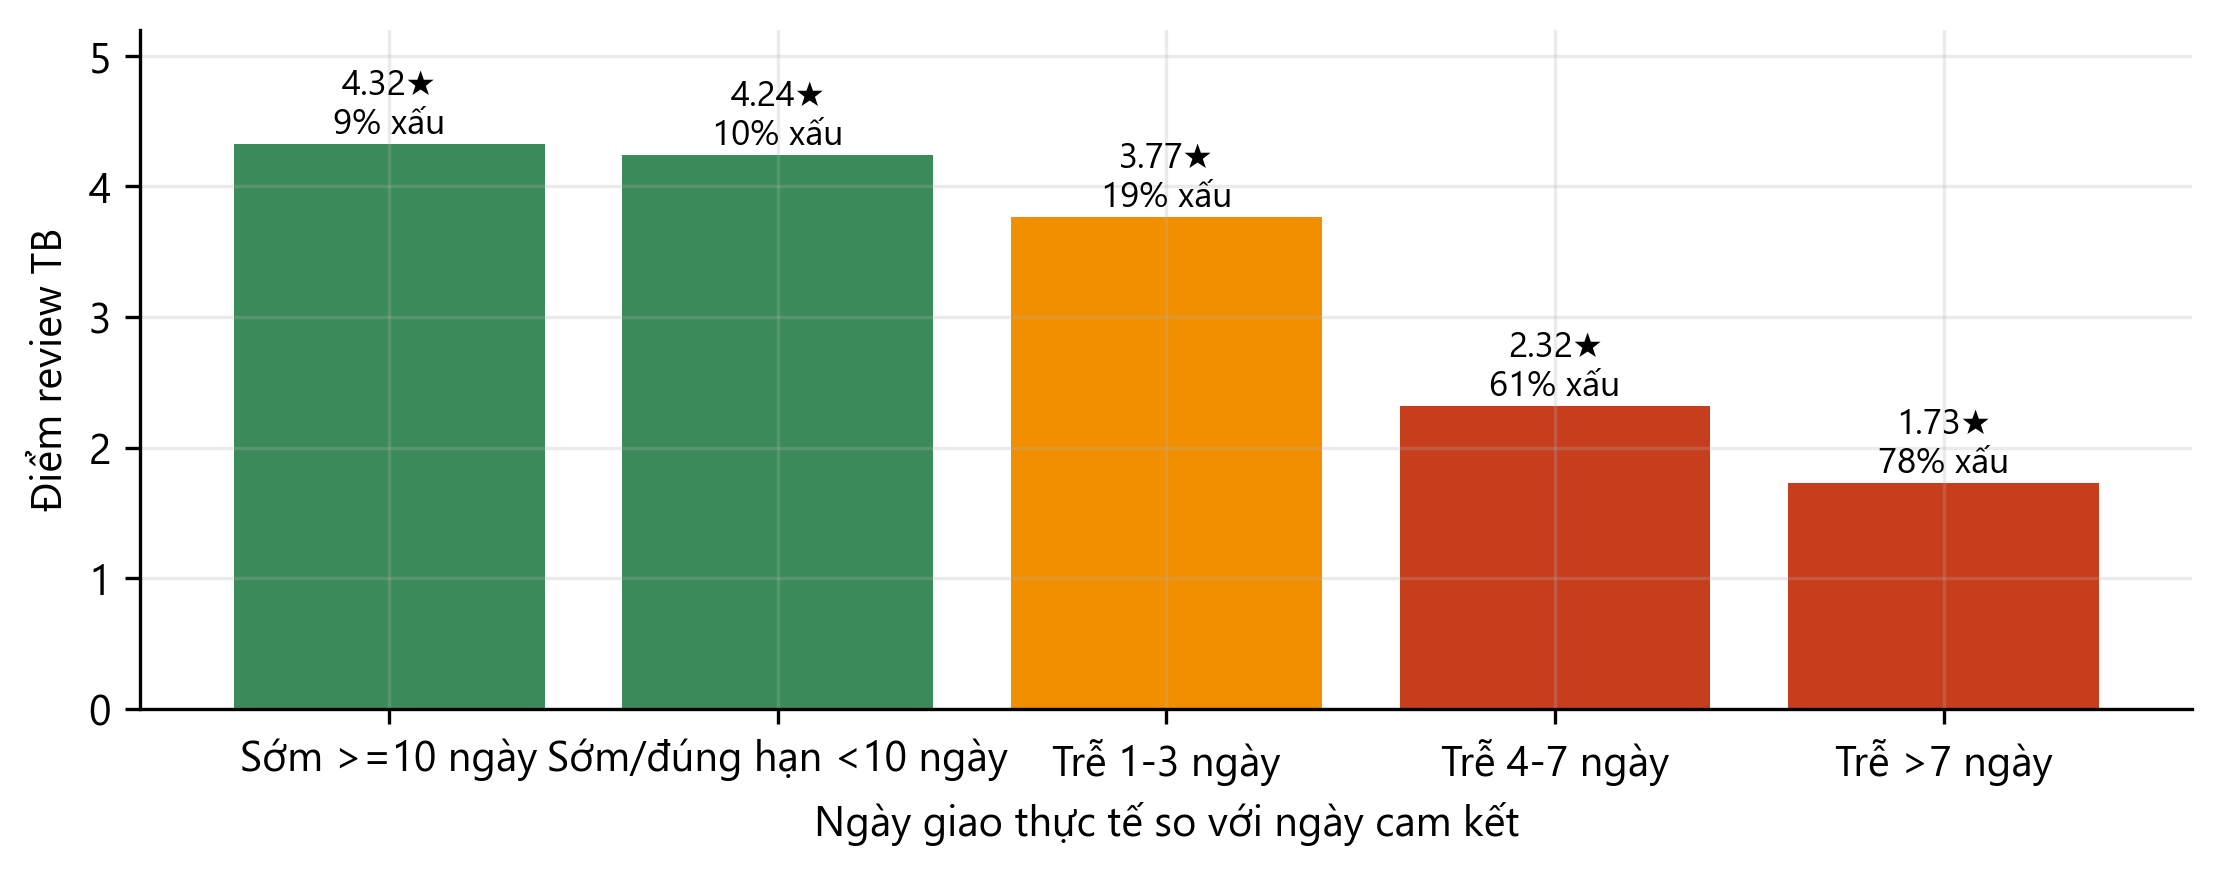
\includegraphics[width=0.75\textwidth]{f2_review_delay.png}
    \caption{Điểm đánh giá trung bình theo mức độ trễ so với ngày cam kết}
    \label{fig:review}
\end{figure}

Ba phát hiện trên định nghĩa ba bài toán quyết định bán cấu trúc, là đầu vào cho Mục~\ref{sec:dss}: (1) \textit{nên cam kết bao nhiêu ngày giao}; (2) \textit{khi có cú sốc}, đơn nào cần can thiệp; (3) \textit{người bán nào} gây ra trễ hạn và đánh giá tiêu cực cần được xử lý.

% ============================================================ 7
\section{Hệ hỗ trợ quyết định}
\label{sec:dss}

\subsection{Kiến trúc DSS và quy trình ra quyết định}
\begin{figure}[!htbp]
    \centering
    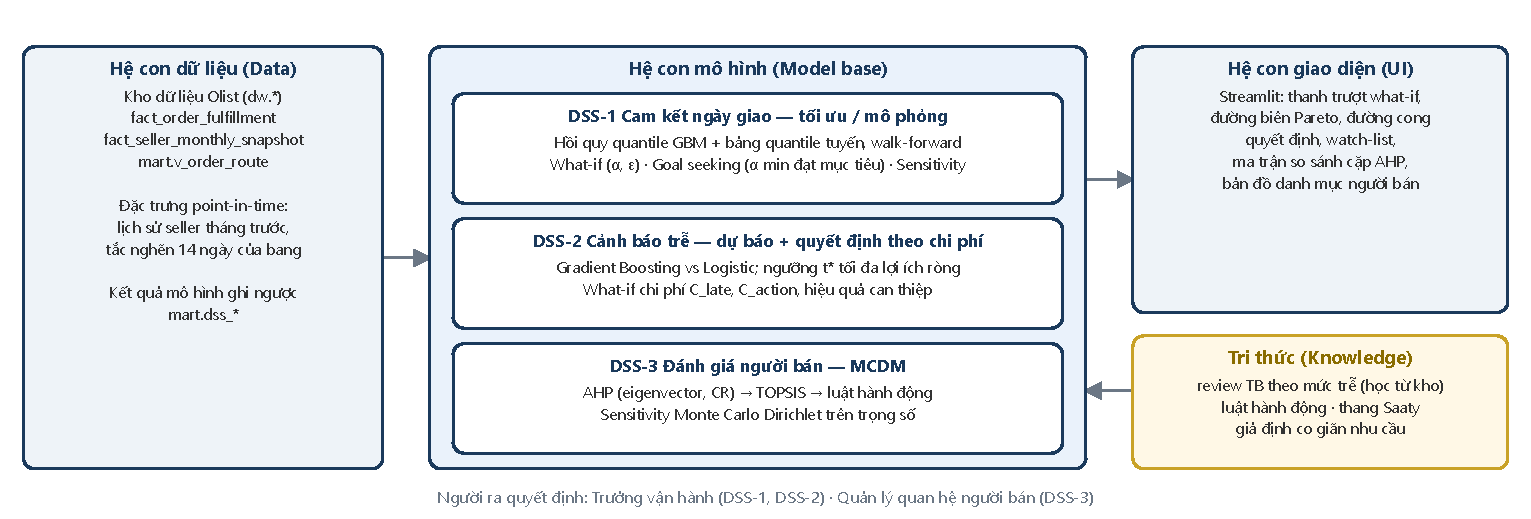
\includegraphics[width=\textwidth]{d_dss_arch.pdf}
    \caption{Kiến trúc DSS theo Turban: hệ con dữ liệu (kho dữ liệu), model base, giao diện và tri thức}
    \label{fig:dss-arch}
\end{figure}

DSS được xây dựng \textbf{trên} kho dữ liệu, đúng với vai trò của DW là hệ con quản lý dữ liệu của DSS (Hình~\ref{fig:dss-arch}). Mọi đặc trưng của mô hình đều được đọc từ các fact và snapshot; kết quả mô hình được script \code{build_dss.py} ghi ngược vào kho (các bảng \code{mart.dss_*}). Nhờ vậy giao diện phản hồi tức thì, trong khi các phép tính what-if nhẹ (trọng số AHP, chi phí, độ co giãn) được tính lại ngay khi người dùng thay đổi tham số. Bảng~\ref{tab:simon} ánh xạ ba mô-đun vào các pha của Simon.

\begin{table}[!htbp]
\centering
\caption{Ánh xạ các mô-đun DSS vào quy trình ra quyết định của Simon}
\label{tab:simon}
\small
\begin{tabularx}{\textwidth}{@{}l Y Y Y@{}}
\toprule
\thead{Pha} & \thead{DSS-1: Cam kết giao} & \thead{DSS-2: Cảnh báo trễ} & \thead{DSS-3: Người bán} \\
\midrule
Intelligence & Cam kết dư khoảng 11 ngày nhưng trễ vẫn tăng vọt khi có cú sốc (Q13) & Trễ trên 7 ngày dẫn tới 1,73 điểm; trễ tập trung theo thời gian và bang & Chênh lệch lớn về đúng hạn, đánh giá, SLA giữa các người bán \\
Design & Biến quyết định: mức phục vụ $\alpha$; mô hình quantile; hai phương án chính sách & Biến quyết định: ngưỡng $t$; mô hình phân loại; ma trận chi phí & Tiêu chí, ma trận so sánh cặp, TOPSIS, luật hành động \\
Choice & Đường biên Pareto, goal seeking $\alpha$, phân tích độ nhạy & Ngưỡng tối đa lợi ích ròng; độ nhạy chi phí & Xếp hạng và đánh giá độ vững Monte Carlo \\
Implementation & Bảng cam kết theo tuyến cho tháng tới & Danh sách cảnh báo hằng ngày & Danh sách hành động cho từng người bán \\
\bottomrule
\end{tabularx}
\end{table}

\subsection{DSS-1: Tối ưu cam kết ngày giao hàng}

\subsubsection{Mô hình hóa}
\begin{itemize}
    \item \textbf{Biến quyết định:} mức phục vụ $\alpha \in [0{,}6;\, 0{,}975]$ và loại chính sách (bảng theo tuyến hoặc mô hình cấp đơn).
    \item \textbf{Biến không kiểm soát được:} phân phối thời gian giao thực tế, phụ thuộc vào tuyến, khoảng cách, khối lượng và mùa vụ.
    \item \textbf{Biến kết quả:} số ngày cam kết trung bình, tỷ lệ đúng hạn, tỷ lệ trễ trên 3 ngày, điểm đánh giá kỳ vọng, chỉ số nhu cầu.
\end{itemize}
Số ngày cam kết cho đơn $i$ với đặc trưng $\mathbf{x}_i$ được xác định bởi quantile có điều kiện của thời gian giao~\cite{koenker1978}:
\begin{equation}
P_i(\alpha) = \left\lceil \hat{Q}_\alpha\!\left(\text{LeadTime} \mid \mathbf{x}_i\right) \right\rceil ,
\end{equation}
trong đó $\hat{Q}_\alpha$ được ước lượng theo hai cách:
\begin{enumerate}[label=(\roman*)]
    \item \textit{Bảng quantile theo tuyến} (bang người bán $\rightarrow$ bang khách hàng); tuyến có dưới 30 đơn dùng phân phối cấp vùng, sau đó cấp toàn quốc (hierarchical fallback). Cách này dễ giải thích.
    \item \textit{Hồi quy quantile Gradient Boosting} tối thiểu hóa hàm mất mát pinball $\rho_\alpha(u) = u\,(\alpha - \mathbf{1}[u<0])$, với các đặc trưng: tuyến, khoảng cách, trọng lượng, phí vận chuyển, giá trị đơn, tháng và thứ trong tuần.
\end{enumerate}
Điểm đánh giá kỳ vọng được tính từ tri thức học được từ kho (Hình~\ref{fig:review}), với $k$ là các mức trễ:
\begin{equation}
\mathbb{E}[\text{Review}] = \sum_{k} \Pr(\text{mức trễ } k) \cdot \overline{\text{Review}}_k .
\end{equation}
Chỉ số nhu cầu là một \textbf{giả định có thể điều chỉnh}, phản ánh việc cam kết dài hơn làm giảm sức hấp dẫn của đơn hàng (mặc định $\varepsilon = 2\%$ mỗi ngày):
\begin{equation}
D = \frac{1}{n}\sum_{i=1}^{n} \exp\!\left(-\varepsilon \left(P_i^{\text{mới}} - P_i^{\text{Olist}}\right)\right).
\end{equation}

\subsubsection{Thiết kế thực nghiệm walk-forward}
DSS-1 và DSS-2 làm việc trên các đơn \textbf{chỉ có một người bán} (khoảng 98\% số đơn), vì chỉ khi đó tuyến nơi gửi $\rightarrow$ nơi nhận mới xác định duy nhất (view \code{mart.v_order_route}). Với mỗi tháng kiểm thử $M$ (03--08/2018, tổng cộng 38.350 đơn), mô hình được huấn luyện lại trên 6 tháng $[M-7, M-1)$ và \textbf{bỏ qua 1 tháng đệm}. Lý do: tại thời điểm ra quyết định, nhiều đơn của tháng gần nhất chưa giao xong (right-censoring); nếu huấn luyện trên chúng, mô hình sẽ bị thiên lệch về phía giao nhanh. Tổng cộng 16 mức $\alpha$ $\times$ 2 chính sách = 1.227.200 dự báo được lưu trong \code{mart.dss_promise_backtest}.

\subsubsection{Kết quả}
\begin{figure}[!htbp]
    \centering
    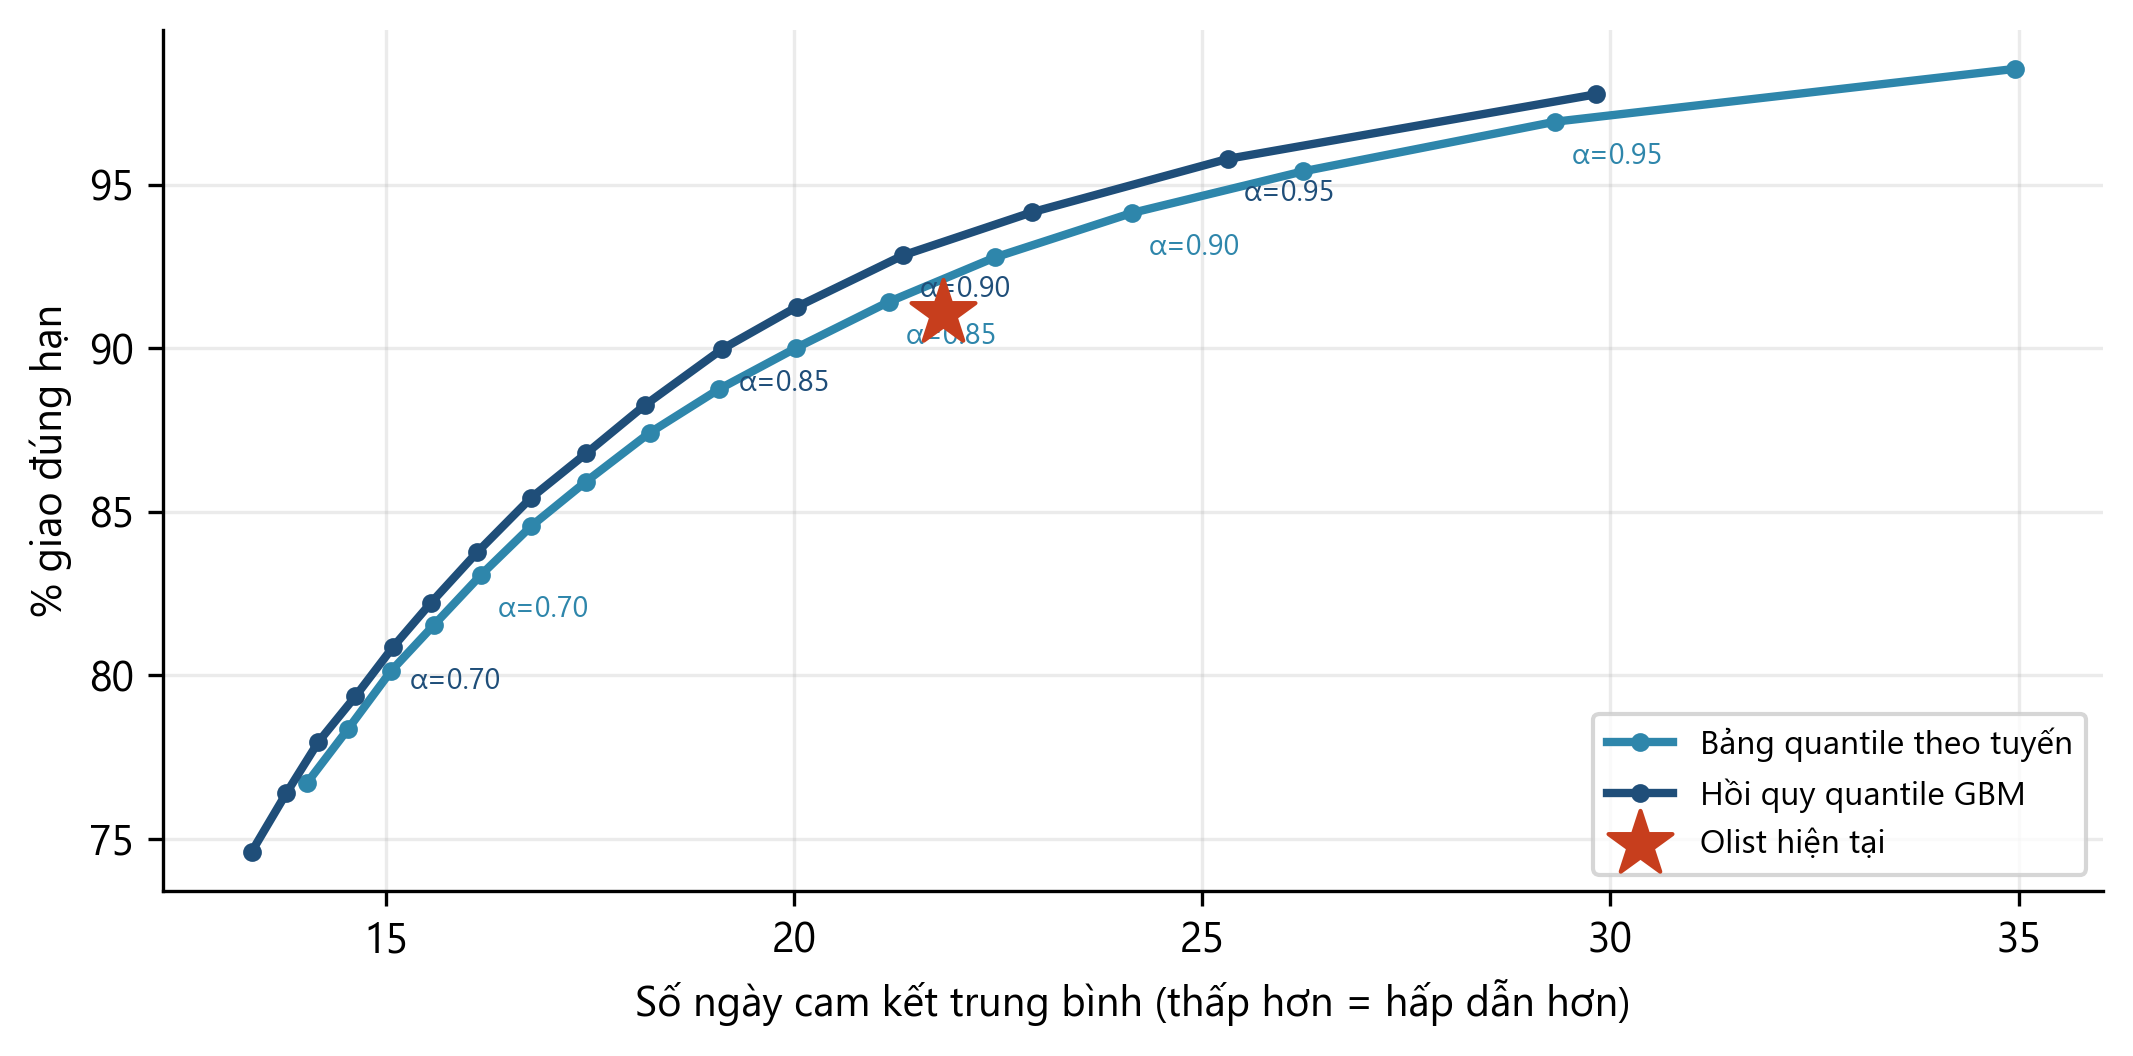
\includegraphics[width=0.85\textwidth]{f4_frontier.png}
    \caption{Đường biên đánh đổi giữa số ngày cam kết và tỷ lệ giao đúng hạn (backtest 03--08/2018); ngôi sao là chính sách hiện tại của Olist}
    \label{fig:frontier}
\end{figure}

\begin{table}[!htbp]
\centering
\caption{So sánh các phương án cam kết với chính sách hiện tại của Olist}
\label{tab:dss1}
\small
\resizebox{\textwidth}{!}{\begin{tabular}{@{}l c c c c c c@{}}
\toprule
\thead{Phương án} & \thead{$\alpha$} & \thead{Cam kết (ngày)} & \thead{Đúng hạn} & \thead{Trễ $>$3 ngày} & \thead{Review kỳ vọng} & \thead{Nhu cầu} \\
\midrule
Olist hiện tại & -- & 21,82 & 91,1\% & 5,5\% & 4,121 & 1,000 \\
Bảng theo tuyến & 0,850 & 21,16 & 91,4\% & 5,6\% & 4,119 & 1,027 \\
GBM -- ``hứa ngắn hơn'' & 0,875 & \textbf{20,03} & 91,3\% & 5,4\% & 4,107 & \textbf{1,051} \\
GBM -- ``đúng hạn hơn'' & 0,900 & 21,33 & \textbf{92,8\%} & \textbf{4,5\%} & \textbf{4,141} & 1,024 \\
GBM -- mục tiêu 95\% & 0,950 & 25,31 & 95,8\% & 2,6\% & 4,218 & 0,948 \\
\bottomrule
\end{tabular}}
\end{table}

Nội suy trên đường biên (Hình~\ref{fig:frontier}, Bảng~\ref{tab:dss1}) cho thấy:
\begin{itemize}
    \item Với cùng tỷ lệ đúng hạn như Olist (91,1\%), mô hình GBM chỉ cần cam kết \textbf{19,9 ngày}, tức ngắn hơn 1,9 ngày (giảm 8,8\%).
    \item Với cùng 21,8 ngày cam kết, tỷ lệ đúng hạn đạt \textbf{93,2\%} (tăng 2,2 điểm phần trăm), tương đương giảm khoảng 24\% số đơn trễ.
    \item Bảng theo tuyến cũng trội hơn Olist nhưng với mức cải thiện nhỏ hơn (20,9 ngày; 92,1\%), đổi lại hoàn toàn giải thích được.
\end{itemize}
Đây là mức cải thiện khiêm tốn nhưng trung thực: chính sách của Olist vốn đã là một mô hình ước lượng. Đóng góp chính của DSS là \textbf{làm minh bạch sự đánh đổi} và cho phép nhà quản lý \textbf{chủ động lựa chọn mức phục vụ}.

\begin{table}[!htbp]
\centering
\caption{Độ bền theo tháng của DSS-1 ($\alpha = 0{,}9$) so với Olist}
\label{tab:dss1-monthly}
\small
\begin{tabular}{@{}l c c c c@{}}
\toprule
\thead{Tháng} & \thead{Olist: cam kết} & \thead{Olist: đúng hạn} & \thead{DSS: cam kết} & \thead{DSS: đúng hạn} \\
\midrule
2018-03 & 22,0 & 78,4\% & 22,7 & 80,5\% \\
2018-04 & 23,6 & 94,6\% & 25,7 & 96,8\% \\
2018-05 & 22,8 & 91,6\% & 25,6 & 95,8\% \\
2018-06 & 27,7 & 98,6\% & 18,7 & 95,3\% \\
2018-07 & 19,7 & 95,5\% & 20,3 & 96,4\% \\
2018-08 & 15,0 & 89,4\% & 14,0 & 93,3\% \\
\bottomrule
\end{tabular}
\end{table}

Bảng~\ref{tab:dss1-monthly} cho thấy DSS tự điều chỉnh theo dữ liệu gần nhất: rút ngắn mạnh cam kết ở 06/2018 (giảm 9,0 ngày) khi vận chuyển nhanh lên, và kéo dài cam kết ở 04--05/2018 sau đợt tắc nghẽn. Backtest cũng chỉ ra một hạn chế quan trọng: ở tháng 03/2018, cả Olist lẫn DSS đều chỉ đạt khoảng 80\% đúng hạn do cú sốc vận chuyển không thể dự báo từ dữ liệu 6 tháng trước. Một mô hình cam kết tĩnh tại thời điểm đặt hàng là chưa đủ -- điều này dẫn trực tiếp tới DSS-2: can thiệp \textit{sau} khi đơn đã được bàn giao.

\subsubsection{What-if, goal seeking và phân tích độ nhạy}
\begin{itemize}
    \item \textbf{What-if:} người dùng thay đổi chính sách, $\alpha$ và độ co giãn $\varepsilon$; mọi chỉ số và đường biên được tính lại tức thì.
    \item \textbf{Goal seeking:} người dùng nhập mục tiêu tỷ lệ đúng hạn (ví dụ 92\%), hệ thống tìm $\alpha$ \textit{nhỏ nhất} (tức cam kết ngắn nhất) đạt mục tiêu: $\alpha = 0{,}90$, tương ứng 21,3 ngày.
    \item \textbf{Phân tích độ nhạy:} bảng mục tiêu đúng hạn từ 85\% đến 96\% kèm $\alpha$ và số ngày cam kết tương ứng; chỉ số nhu cầu theo $\varepsilon \in \{0; 1; 2; 3; 5\}\%$. Kết luận về chiều hướng (mô hình trội hơn Olist) \textit{không} phụ thuộc vào $\varepsilon$; $\varepsilon$ chỉ thay đổi độ lớn của lợi ích.
\end{itemize}

\begin{figure}[!htbp]
    \centering
    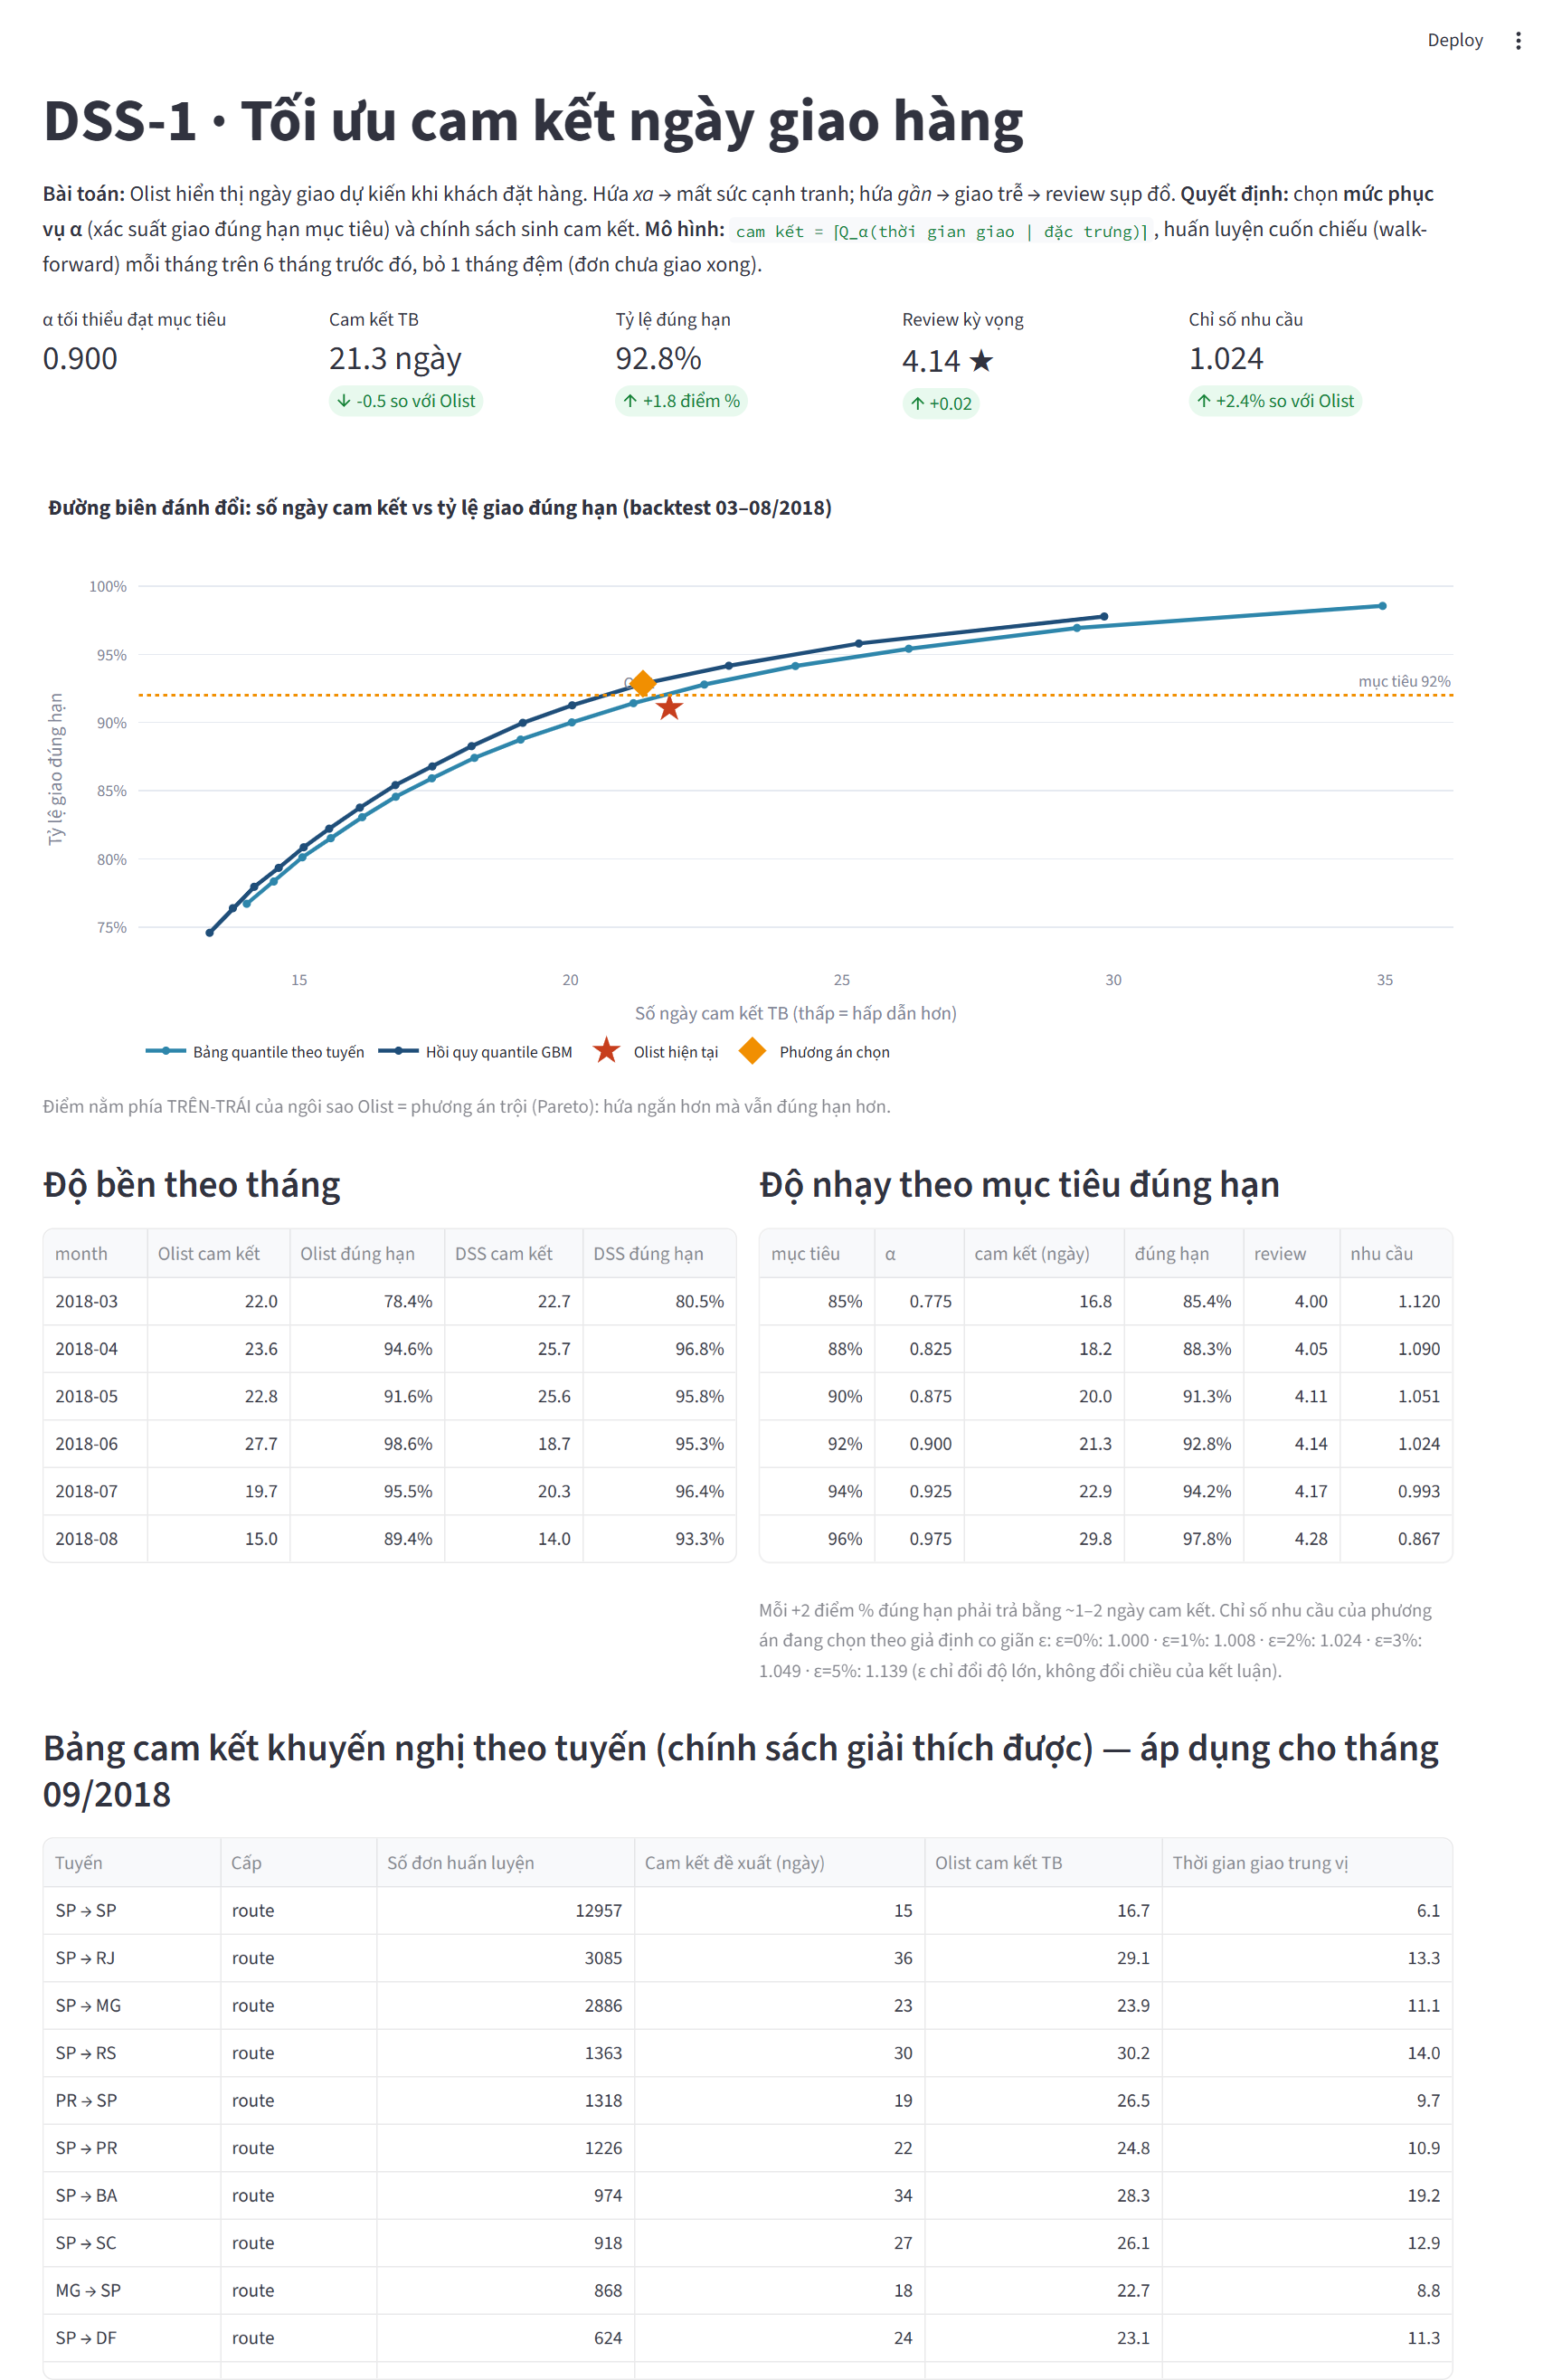
\includegraphics[width=0.9\textwidth,trim=0 1420 0 0,clip]{dss1_c.png}
    \caption{Giao diện DSS-1: chỉ số so sánh với Olist, đường biên Pareto, độ bền theo tháng và phân tích độ nhạy}
    \label{fig:dash-dss1}
\end{figure}

\subsection{DSS-2: Cảnh báo sớm đơn có nguy cơ giao trễ}

\subsubsection{Mô hình hóa và quá trình lặp thiết kế}
\textbf{Quyết định:} với mỗi đơn vừa được bàn giao cho hãng vận chuyển, có can thiệp hay không (nâng cấp dịch vụ vận chuyển, chủ động thông báo cho khách, nhắc nhở người bán).

\textbf{Thiết kế ban đầu} chấm điểm rủi ro tại thời điểm \textit{duyệt đơn} chỉ đạt ROC-AUC 0,65, vì nguyên nhân trễ chủ yếu là các cú sốc hệ thống chưa xảy ra tại thời điểm duyệt. Nhóm vì vậy \textbf{dời thời điểm quyết định sang mốc bàn giao vận chuyển} (một mốc của accumulating snapshot) và bổ sung các nhóm đặc trưng \textit{point-in-time}:
\begin{itemize}
    \item \code{slack_days} = ngày cam kết $-$ ngày bàn giao, tức số ngày ``đệm'' còn lại của đơn;
    \item \textbf{Mức tắc nghẽn của bang nhận}: thời gian vận chuyển trung bình, tỷ lệ trễ và số đơn của các đơn \textit{đã giao} trong \textbf{14 ngày trước} ngày bàn giao (cửa sổ trượt không bao gồm ngày hiện tại, nên không rò rỉ dữ liệu);
    \item \textbf{Lịch sử người bán} lấy từ periodic snapshot của \textbf{tháng trước} (tỷ lệ trễ, điểm đánh giá, tỷ lệ vi phạm SLA, có làm trơn Bayes với $k = 10$ về trung bình toàn sàn) và thâm niên;
    \item Đặc trưng của đơn: tuyến, khoảng cách, trọng lượng, phí, giá trị, số sản phẩm, nhóm ngành, ngày lễ, giờ/thứ/tháng đặt hàng.
\end{itemize}
Dữ liệu được chia theo thời gian: huấn luyện trên năm 2017 (42.947 đơn), validation trên 01--02/2018 (để chọn ngưỡng), kiểm thử trên 03--08/2018 (38.350 đơn chưa từng thấy). Hai mô hình được so sánh: Logistic Regression (mã hóa one-hot, chuẩn hóa) và Histogram Gradient Boosting.

\subsubsection{Kết quả mô hình}
\begin{table}[!htbp]
\centering
\caption{Hiệu năng các mô hình cảnh báo trễ}
\label{tab:dss2}
\small
\resizebox{\textwidth}{!}{\begin{tabular}{@{}l l c c c c c@{}}
\toprule
\thead{Mô hình} & \thead{Tập} & \thead{\% trễ} & \thead{ROC-AUC} & \thead{PR-AUC} & \thead{Lift top-10\%} & \thead{Recall top-10\%} \\
\midrule
Logistic Regression & Validation & 9,9\% & 0,754 & 0,306 & 3,12 & 31,2\% \\
Logistic Regression & Test & 7,1\% & 0,724 & 0,224 & 3,11 & 31,1\% \\
Gradient Boosting & Validation & 9,9\% & 0,719 & 0,311 & 3,37 & 33,7\% \\
\textbf{Gradient Boosting} & \textbf{Test} & 7,1\% & \textbf{0,768} & \textbf{0,327} & \textbf{3,77} & \textbf{37,7\%} \\
\bottomrule
\end{tabular}}
\end{table}
Mô hình được chọn trên tập \textbf{validation}, theo PR-AUC và lift top-10\% -- hai chỉ số sát với bài toán gắn cờ một tỷ lệ nhỏ đơn: Gradient Boosting cao hơn Logistic Regression ở cả hai (0,311 so với 0,306; 3,37 so với 3,12), dù ROC-AUC thấp hơn (Bảng~\ref{tab:dss2}). Tập kiểm thử xác nhận lựa chọn này: 10\% đơn có rủi ro cao nhất chứa 37,7\% tổng số đơn trễ (gấp 3,8 lần chọn ngẫu nhiên); PR-AUC đạt 0,327 so với mức nền 0,071. Các đặc trưng quan trọng nhất là \code{slack_days}, bang nhận và mức tắc nghẽn 14 ngày -- khẳng định giá trị của các đặc trưng được dựng từ kho dữ liệu.

\subsubsection{Lựa chọn ngưỡng theo chi phí}
Lợi ích ròng tại ngưỡng $t$ được định nghĩa:
\begin{equation}
B(t) = \text{TP}(t)\cdot C_{\text{late}}\cdot e \;-\; \big(\text{TP}(t) + \text{FP}(t)\big)\cdot C_{\text{action}},
\end{equation}
với giả định mặc định $C_{\text{late}} = 25$ BRL (bồi thường và mất khách), $C_{\text{action}} = 4$ BRL và hiệu quả can thiệp $e = 50\%$. Khi đó precision hòa vốn là $C_{\text{action}}/(C_{\text{late}}\, e) = 32\%$. Ngưỡng tối ưu chọn trên tập validation là $t^* = 0{,}21$; áp dụng lên tập kiểm thử: gắn cờ \textbf{3,5\%} số đơn (1.360 đơn), \textbf{precision 45,0\%} (vượt mức hòa vốn), recall 22,3\%, \textbf{lợi ích ròng dương 2.210 BRL} trong 6 tháng trên mẫu dữ liệu.

\begin{figure}[!htbp]
    \centering
    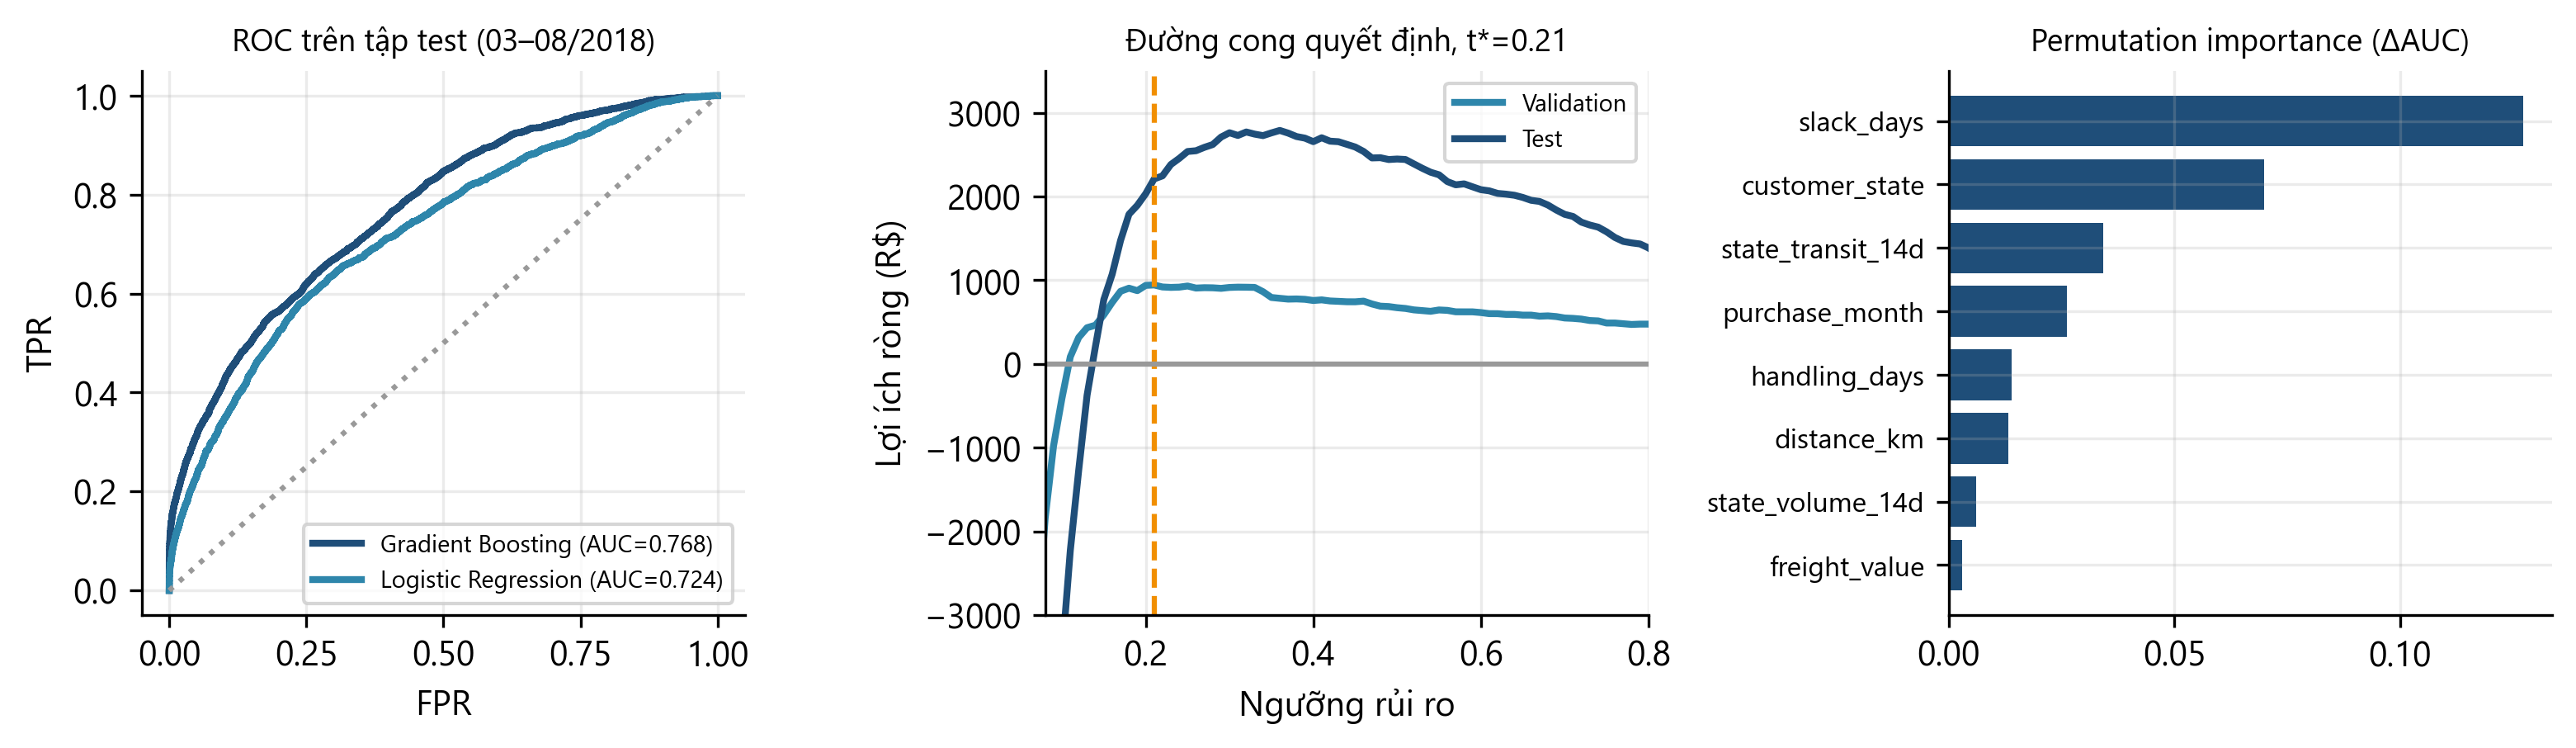
\includegraphics[width=\textwidth]{f5_dss2.png}
    \caption{Đường ROC trên tập kiểm thử; đường cong quyết định (lợi ích ròng theo ngưỡng); mức quan trọng của đặc trưng}
    \label{fig:dss2}
\end{figure}

\begin{table}[!htbp]
\centering
\caption{Phân tích độ nhạy theo chi phí (hiệu quả can thiệp 50\%)}
\label{tab:dss2-sens}
\small
\begin{tabular}{@{}c c c c c r@{}}
\toprule
\thead{$C_{\text{late}}$} & \thead{$C_{\text{action}}$} & \thead{$t^*$} & \thead{\% gắn cờ} & \thead{Precision} & \thead{Lợi ích ròng (BRL)} \\
\midrule
15 & 2 & 0,17 & 5,0\% & 38,2\% & 1.648 \\
15 & 8 & -- & 0\% & -- & 0 \\
25 & 2 & 0,10 & 11,2\% & 25,5\% & 5.104 \\
\textbf{25} & \textbf{4} & \textbf{0,21} & \textbf{3,5\%} & \textbf{45,0\%} & \textbf{2.210} \\
40 & 4 & 0,11 & 9,8\% & 27,2\% & 5.424 \\
40 & 2 & 0,05 & 27,1\% & 16,1\% & 12.746 \\
\bottomrule
\end{tabular}
\end{table}
Bảng~\ref{tab:dss2-sens} cho thấy khi chi phí can thiệp cao so với thiệt hại (15/8), precision hòa vốn là $8/(15 \cdot 0{,}5) \approx 107\% > 100\%$: không ngưỡng nào có lãi, nên DSS khuyến nghị \textit{không} can thiệp (lợi ích 0) -- phương án này luôn nằm trong tập lựa chọn, và cũng là một kết luận quản trị có giá trị.

\begin{figure}[!htbp]
    \centering
    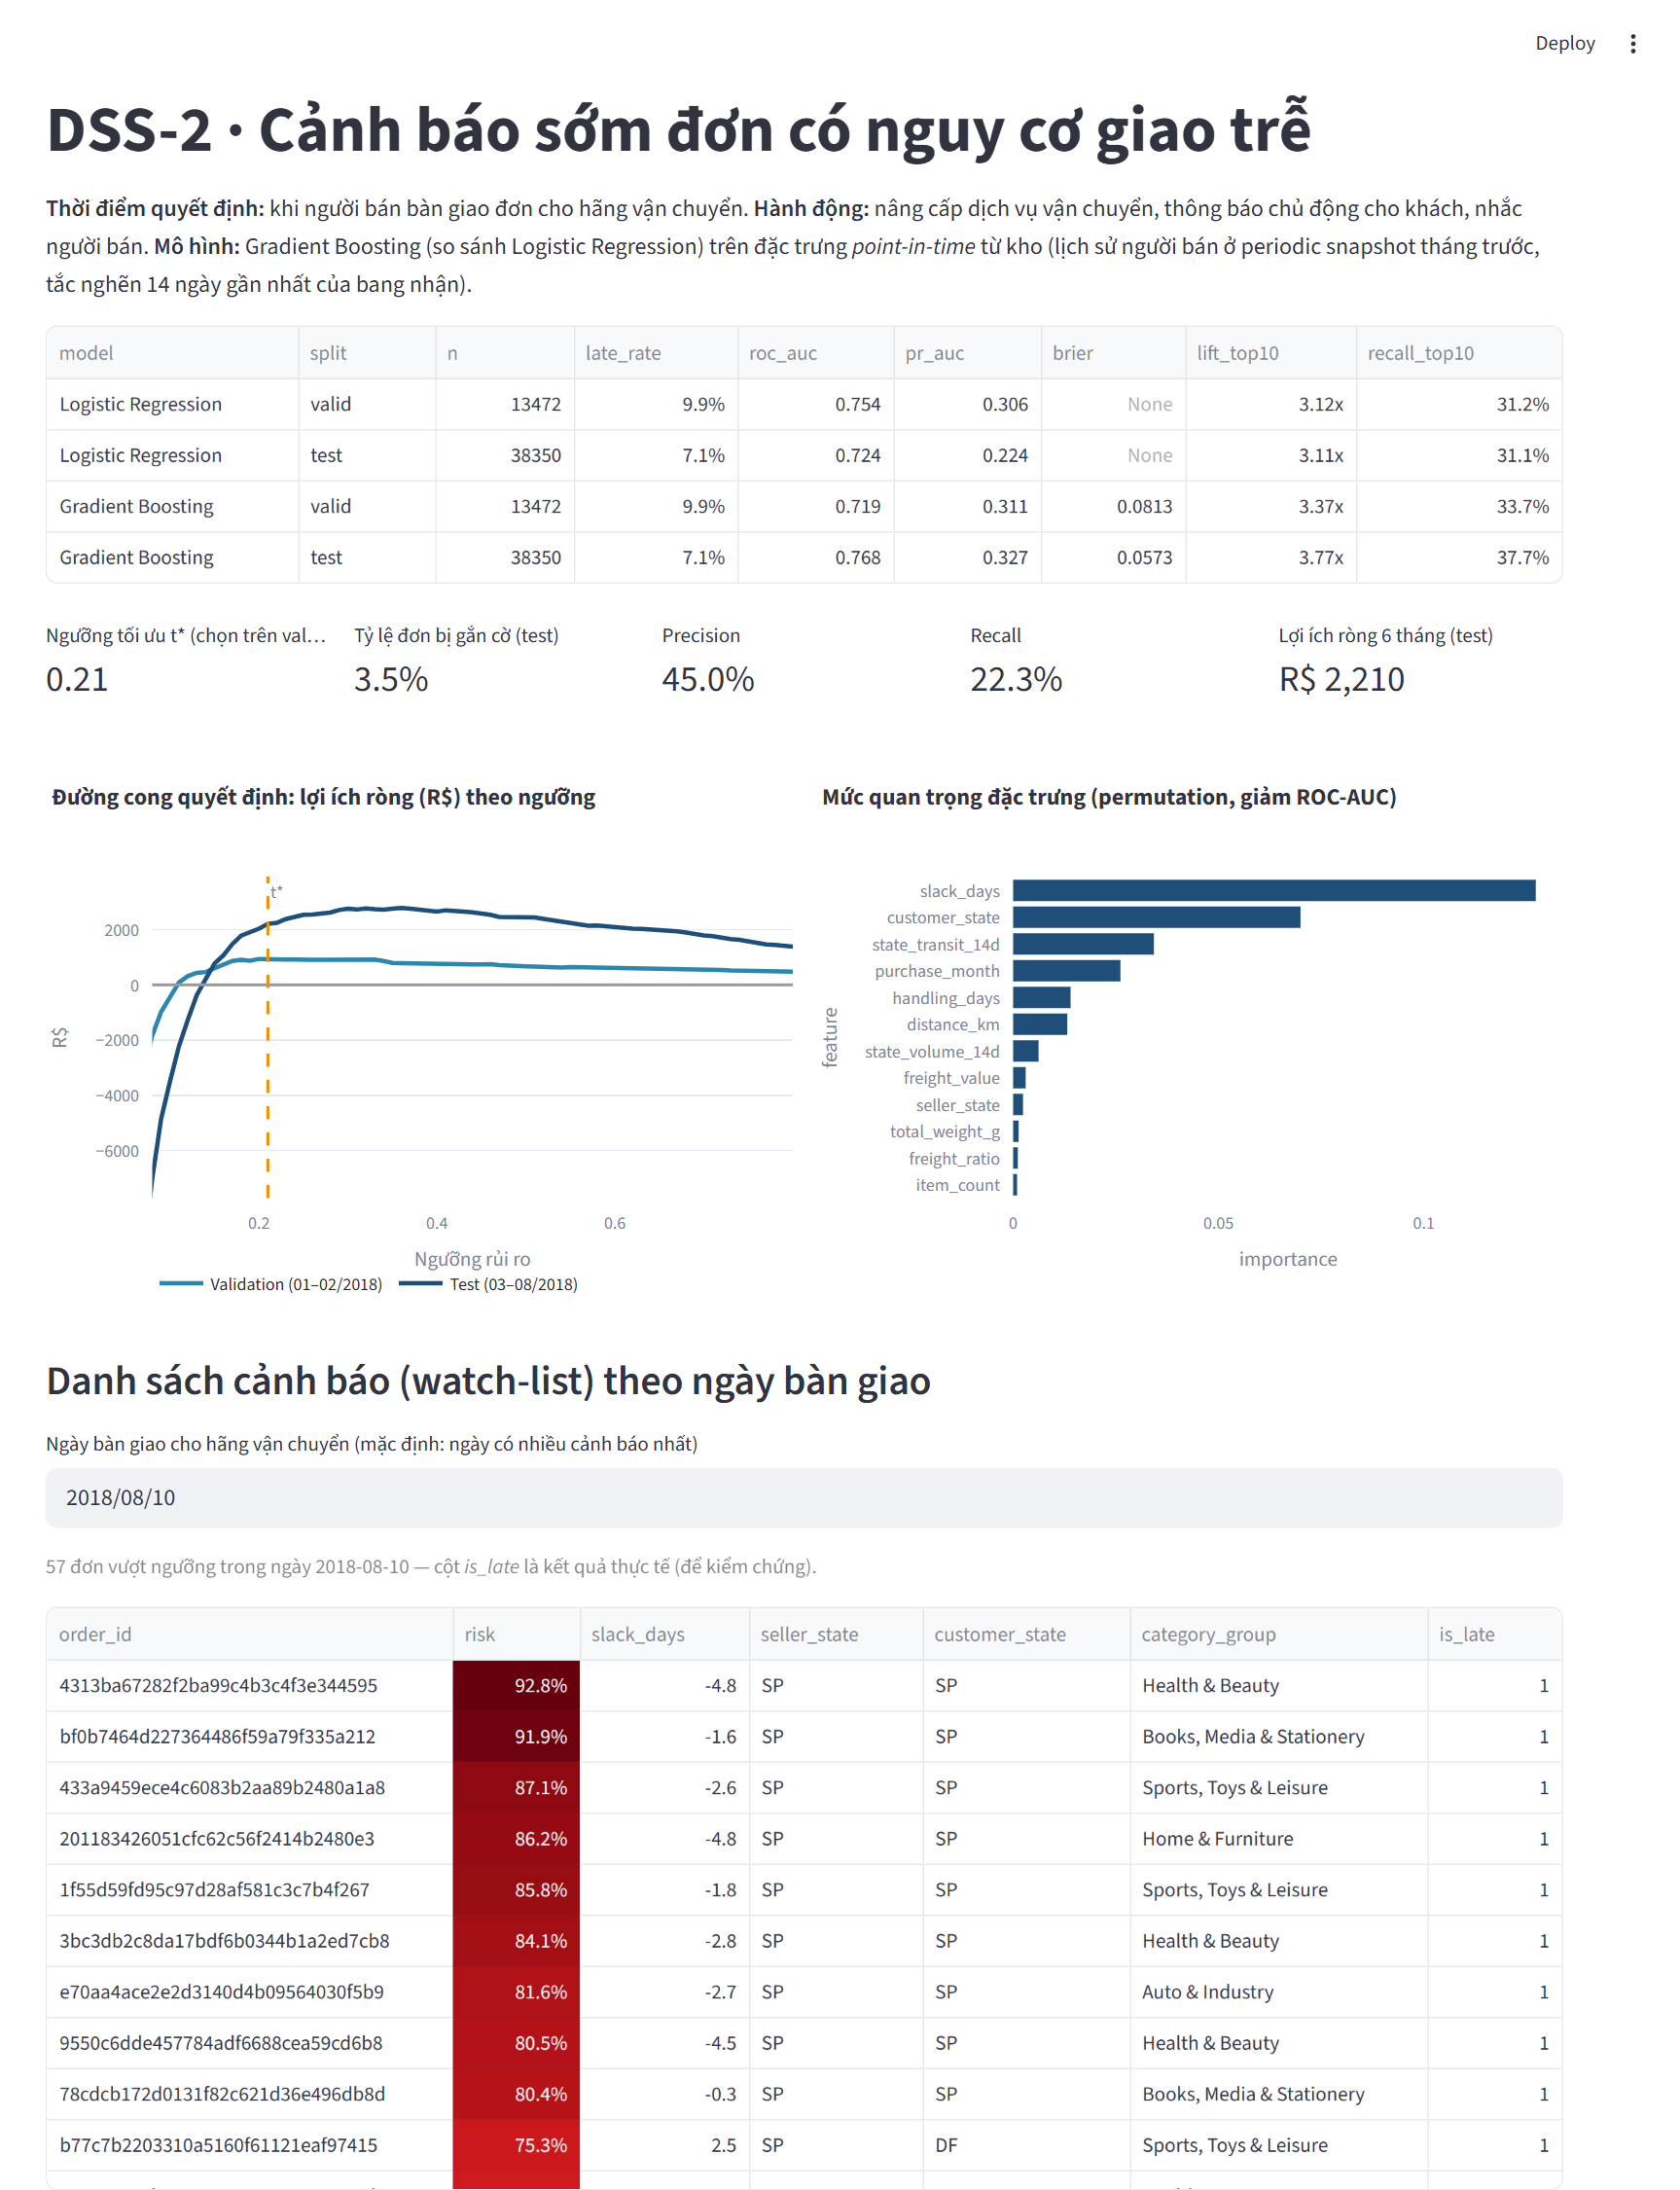
\includegraphics[width=0.9\textwidth]{dss2_c.png}
    \caption{Giao diện DSS-2 với danh sách cảnh báo ngày 10/08/2018: các đơn rủi ro cao đều có \code{slack_days} âm (đã quá ngày cam kết ngay khi bàn giao)}
    \label{fig:dash-dss2}
\end{figure}

\subsection{DSS-3: Đánh giá và phân loại người bán bằng AHP và TOPSIS}

\subsubsection{Mô hình hóa}
\textbf{Phương án:} 444 người bán có ít nhất 20 đơn trong 6 tháng (03--08/2018). \textbf{Tiêu chí} được tính từ periodic snapshot (cộng tử số và mẫu số trước rồi mới chia): GMV (lợi ích, lấy log), tăng trưởng 3 tháng gần nhất so với 3 tháng trước (lợi ích, lấy log), tỷ lệ đúng hạn (lợi ích, phân bổ qua bridge), điểm đánh giá trung bình (lợi ích), tỷ lệ vi phạm SLA (chi phí), tỷ lệ hủy (chi phí).

\textbf{AHP:} nhà quản lý nhập ma trận so sánh cặp $A = [a_{ij}]$ theo thang Saaty 1--9 trên giao diện. Ma trận mặc định (Bảng~\ref{tab:ahp}) phản ánh quan điểm ``trải nghiệm khách hàng là ưu tiên'' -- ví dụ, điểm đánh giá quan trọng gấp 3 lần GMV và gấp 2 lần tỷ lệ đúng hạn. Vector trọng số $\mathbf{w}$ là vector riêng ứng với trị riêng lớn nhất $\lambda_{\max}$, đã chuẩn hóa; tính nhất quán được kiểm tra bằng:
\begin{equation}
CI = \frac{\lambda_{\max} - n}{n - 1}, \qquad CR = \frac{CI}{RI_n}, \qquad RI_6 = 1{,}24 .
\end{equation}

\begin{table}[!htbp]
\centering
\caption{Ma trận so sánh cặp mặc định và trọng số AHP}
\label{tab:ahp}
\small
\begin{tabular}{@{}l c c c c c c r@{}}
\toprule
 & \thead{GMV} & \thead{Tăng trưởng} & \thead{Đúng hạn} & \thead{Đánh giá} & \thead{SLA} & \thead{Hủy} & \thead{Trọng số} \\
\midrule
GMV & 1 & 2 & 1/2 & 1/3 & 1 & 1 & 11,97\% \\
Tăng trưởng & 1/2 & 1 & 1/3 & 1/4 & 1/2 & 1/2 & 6,78\% \\
Đúng hạn & 2 & 3 & 1 & 1/2 & 2 & 2 & 21,84\% \\
Đánh giá & 3 & 4 & 2 & 1 & 3 & 3 & \textbf{35,47\%} \\
SLA & 1 & 2 & 1/2 & 1/3 & 1 & 1 & 11,97\% \\
Hủy & 1 & 2 & 1/2 & 1/3 & 1 & 1 & 11,97\% \\
\bottomrule
\end{tabular}
\end{table}
Kết quả: $\lambda_{\max} = 6{,}032$; $CI = 0{,}0065$; $\mathbf{CR = 0{,}0052 < 0{,}10}$, tức ma trận nhất quán. Nếu người dùng nhập ma trận có $CR \ge 0{,}10$, giao diện sẽ cảnh báo và yêu cầu xem lại các phán đoán.

\textbf{TOPSIS:} ma trận quyết định được chuẩn hóa min--max (vì các tiêu chí lấy log có thể âm) thành $r_{ij}$, nhân trọng số $v_{ij} = w_j r_{ij}$, rồi tính khoảng cách Euclid tới phương án lý tưởng $A^+$ và phản lý tưởng $A^-$:
\begin{equation}
d_i^{\pm} = \sqrt{\sum_j \left(v_{ij} - v_j^{\pm}\right)^2}, \qquad C_i = \frac{d_i^-}{d_i^+ + d_i^-} \in [0, 1].
\end{equation}
\textbf{Luật hành động} (hệ con tri thức): người bán thuộc Top 15\% và không có ``cờ đỏ'' được xếp vào nhóm \textit{Chiến lược}; người bán thuộc Bottom 15\% hoặc có cờ đỏ (đánh giá $< 3{,}5$, đúng hạn $< 85\%$ hoặc vi phạm SLA $> 25\%$) được xếp vào nhóm \textit{Can thiệp}; số còn lại thuộc nhóm \textit{Duy trì} hoặc \textit{Theo dõi}.

\subsubsection{Kết quả}
\begin{figure}[!htbp]
    \centering
    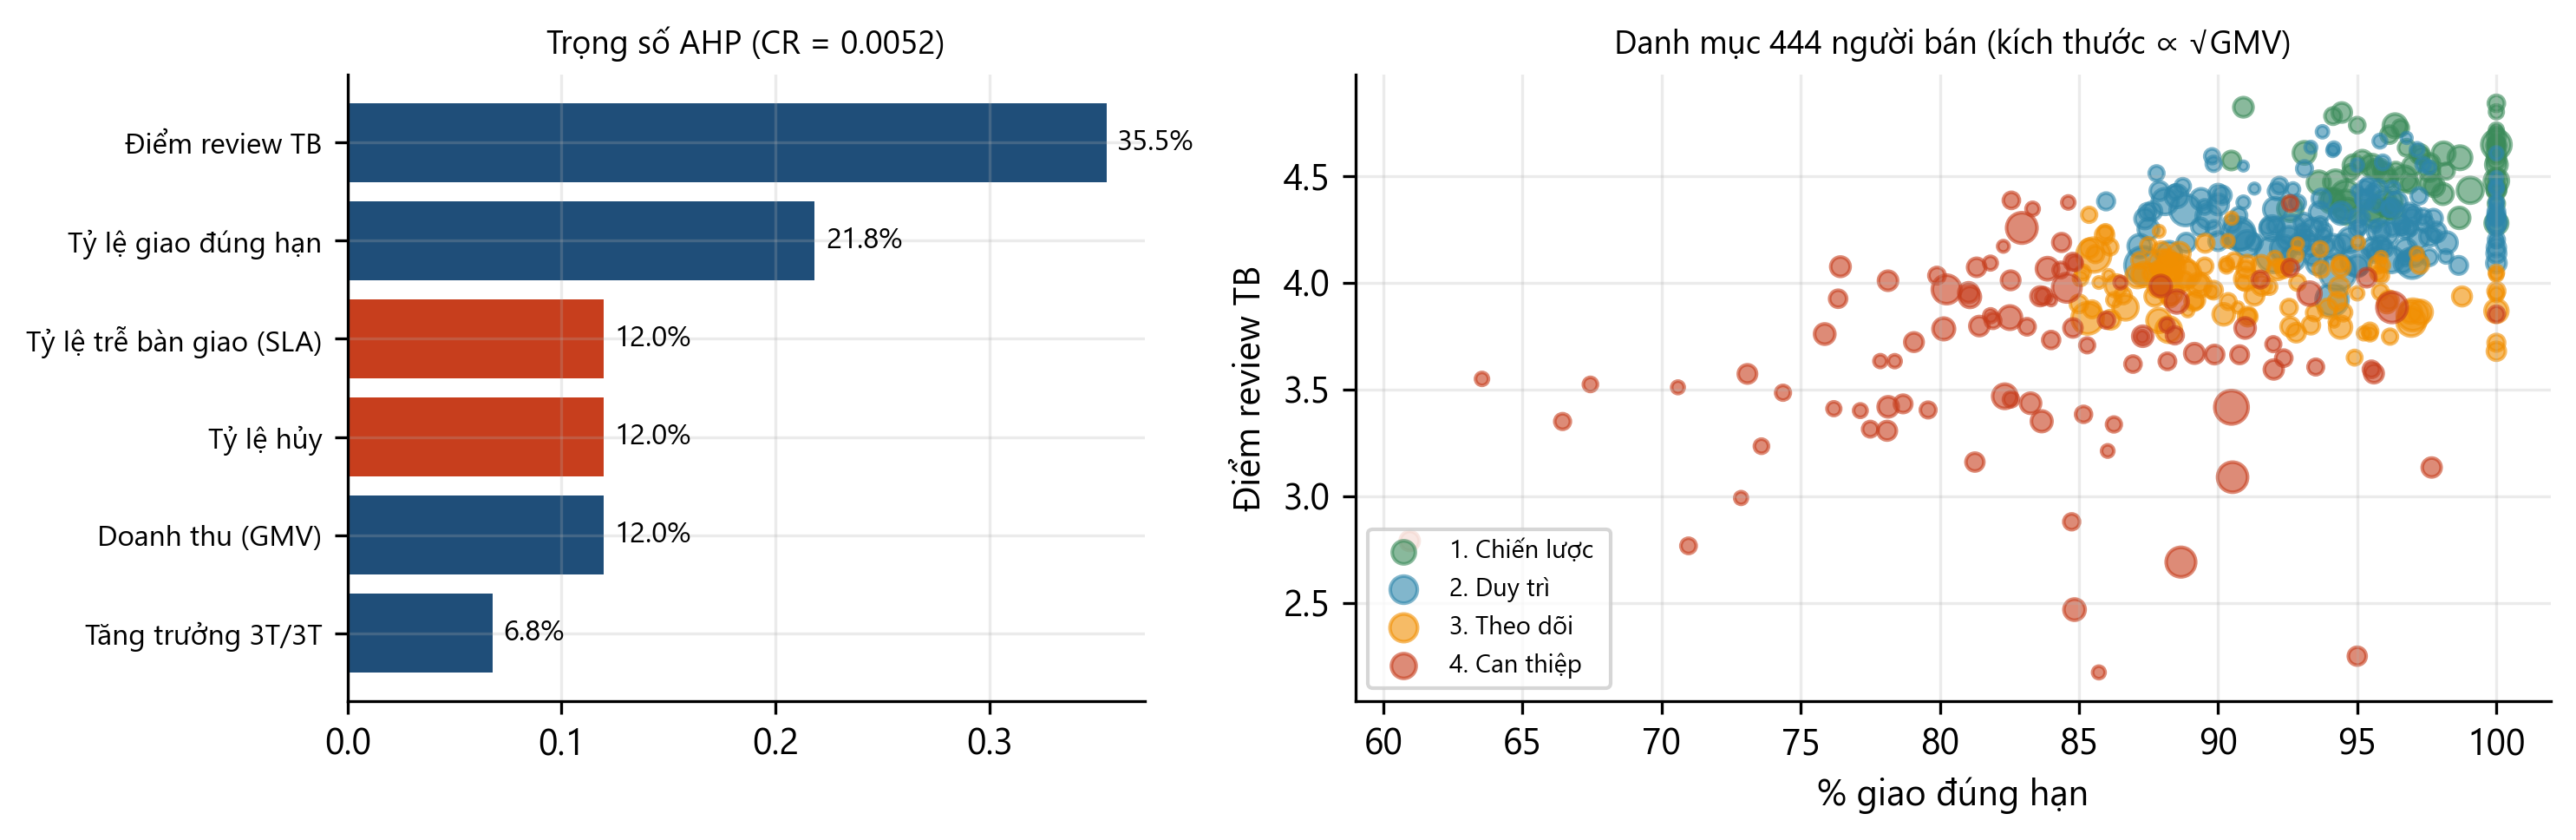
\includegraphics[width=\textwidth]{f6_dss3.png}
    \caption{Trọng số AHP và bản đồ danh mục người bán theo nhóm hành động}
    \label{fig:dss3}
\end{figure}

\begin{table}[!htbp]
\centering
\caption{Đặc điểm trung bình của các nhóm hành động}
\label{tab:dss3}
\small
\resizebox{\textwidth}{!}{\begin{tabular}{@{}l c c r c c c@{}}
\toprule
\thead{Nhóm hành động} & \thead{Số người bán} & \thead{Số đơn} & \thead{GMV (BRL)} & \thead{Đúng hạn} & \thead{Đánh giá} & \thead{Vi phạm SLA} \\
\midrule
1. Chiến lược & 67 & 64 & 10.426 & 97,0\% & 4,54 & 3,6\% \\
2. Duy trì & 154 & 76 & 9.189 & 94,3\% & 4,30 & 5,2\% \\
3. Theo dõi & 126 & 74 & 8.060 & 91,2\% & 3,99 & 5,6\% \\
4. Can thiệp & 97 & 57 & 7.794 & 83,7\% & 3,66 & 16,3\% \\
\bottomrule
\end{tabular}}
\end{table}
Các nhóm tách biệt rõ trên mọi tiêu chí (Bảng~\ref{tab:dss3}). Nhóm Can thiệp có tỷ lệ vi phạm SLA cao gấp 4,5 lần nhóm Chiến lược, gợi ý các hành động cụ thể như đào tạo quy trình đóng gói và bàn giao, hoặc giới hạn hiển thị cho tới khi cải thiện.

\textbf{Phân tích độ nhạy:} thực hiện 500 lần lấy mẫu trọng số $\mathbf{w}' \sim \text{Dirichlet}(50\,\mathbf{w})$ quanh trọng số AHP. Hệ số tương quan hạng Spearman giữa xếp hạng gốc và xếp hạng sau nhiễu có \textbf{trung vị 0,974} và phân vị 5\% là 0,895, cho thấy khuyến nghị \textbf{vững} trước các sai lệch nhỏ trong phán đoán. Giao diện còn hiển thị xác suất mỗi người bán giữ được vị trí Top-$K$: hai người bán dẫn đầu giữ Top-20 ở 100\% và 99,6\% số lần mô phỏng, trong khi một số người bán xếp hạng 15--25 dao động -- đây là các trường hợp ``giáp ranh'' cần nhà quản lý xem xét thủ công.

\begin{figure}[!htbp]
    \centering
    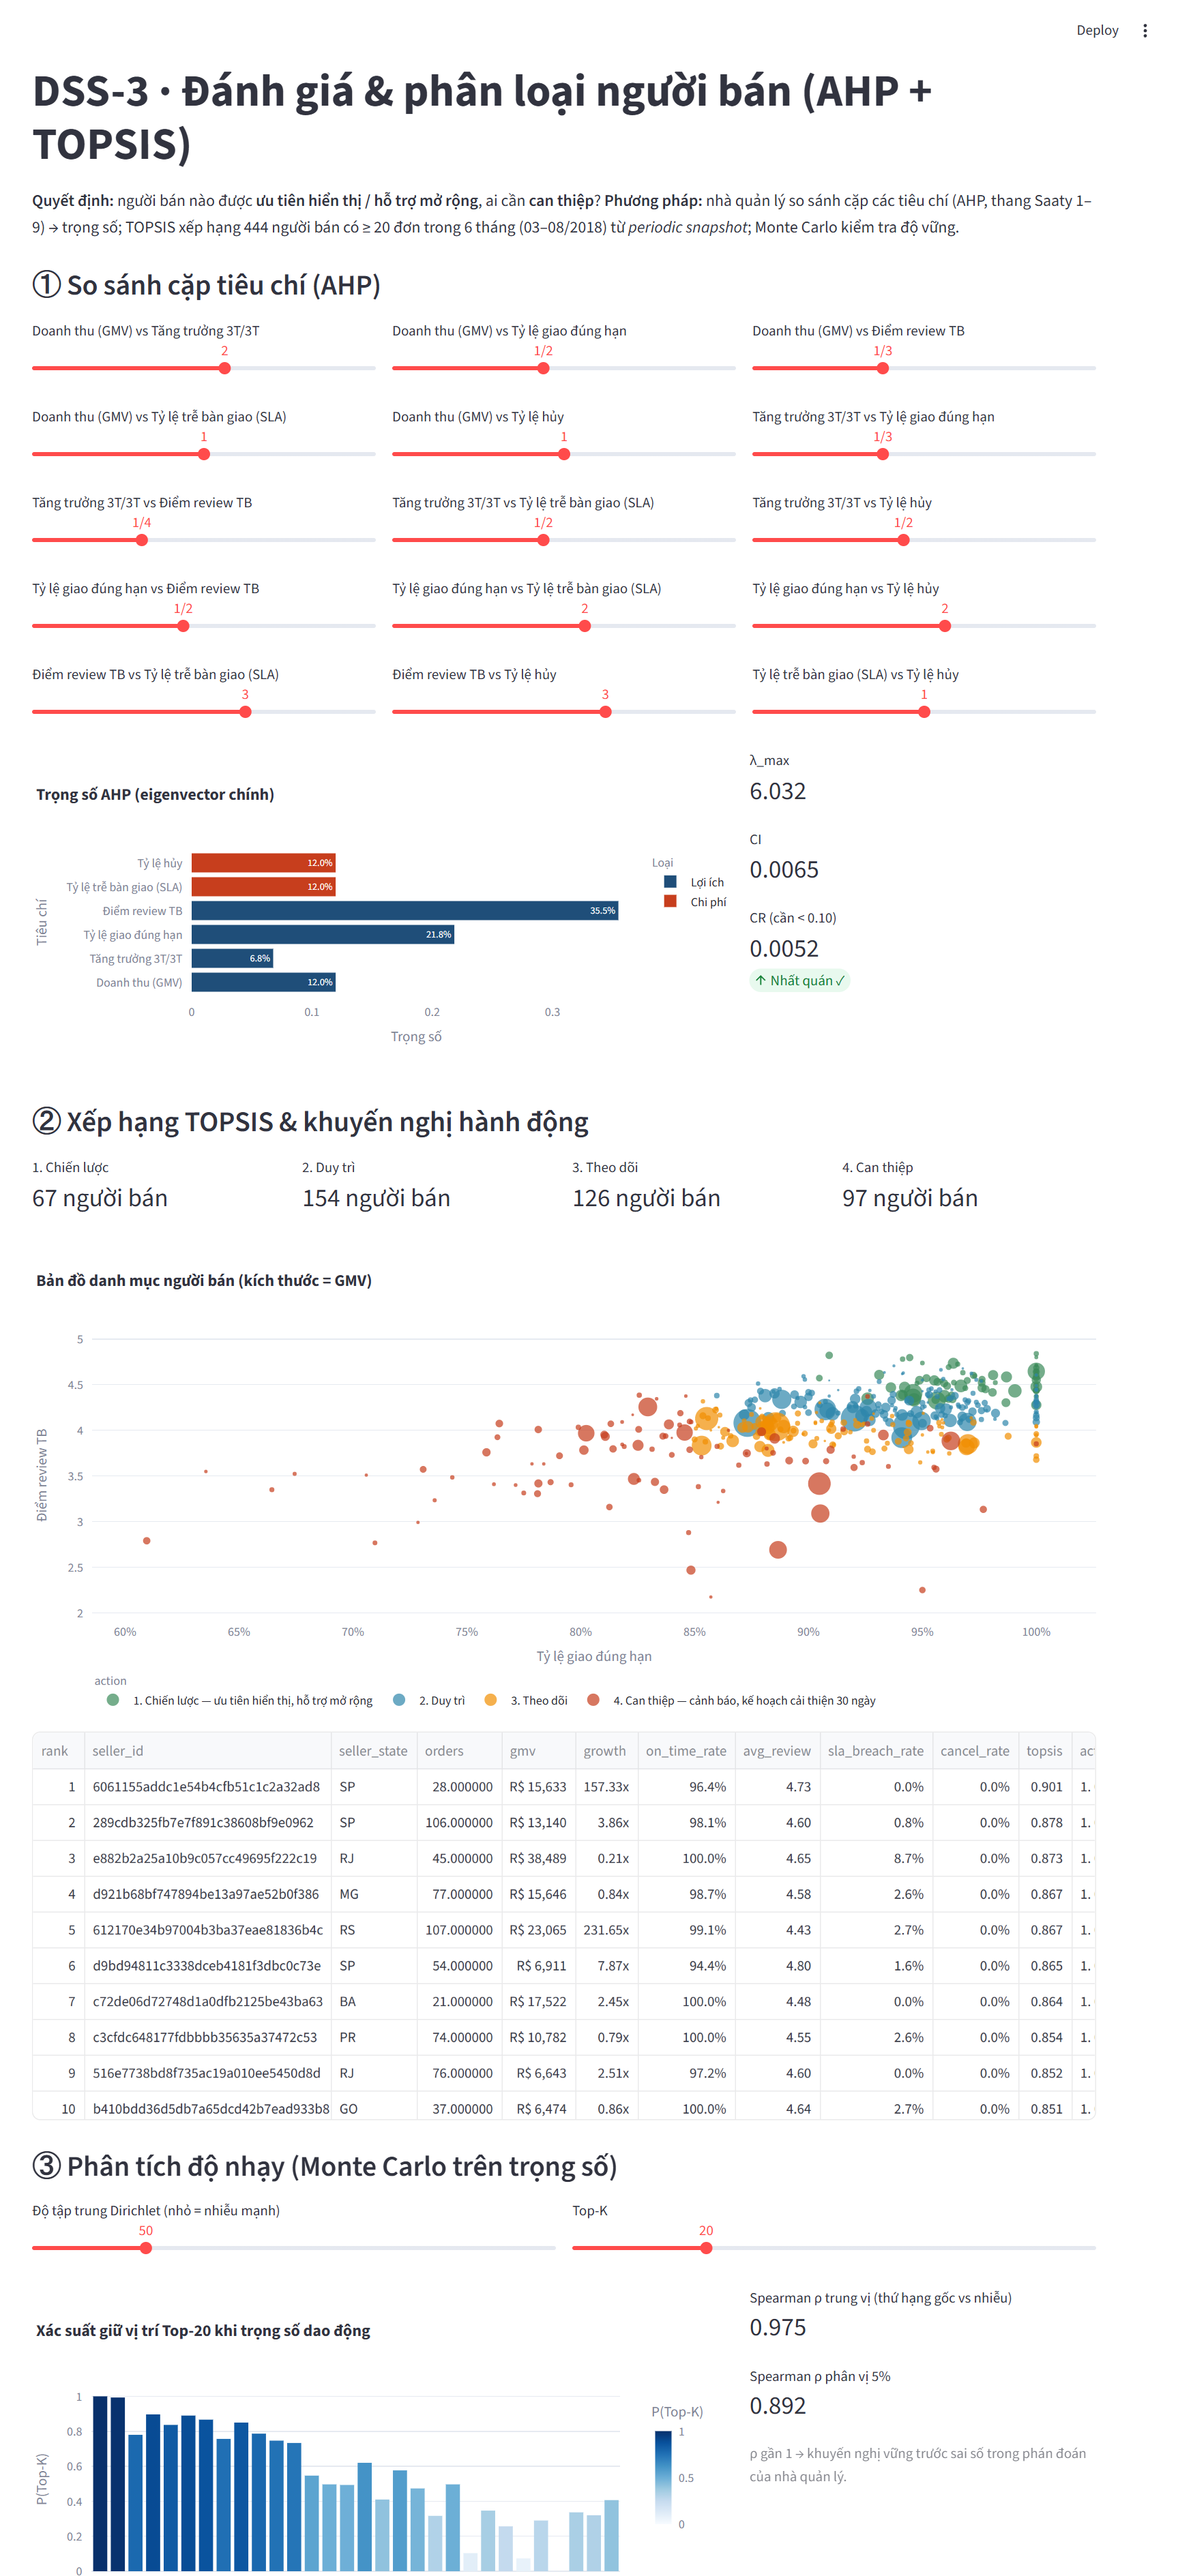
\includegraphics[width=0.85\textwidth,trim=0 1298 0 0,clip]{dss3_c.png}
    \caption{Giao diện DSS-3: ma trận so sánh cặp tương tác, trọng số và chỉ số nhất quán, xếp hạng TOPSIS}
    \label{fig:dash-dss3}
\end{figure}

% ============================================================ 8
\section{Đánh giá, hạn chế và hướng phát triển}

\subsection{Kiểm thử}
Bộ kiểm thử tự động \code{test_warehouse.py} (pytest) gồm \textbf{24 test, tất cả đều đạt}, bao gồm:
\begin{itemize}
    \item tính duy nhất của grain trên 5 bảng fact và bridge table;
    \item không có kiểm tra chất lượng nào thất bại; mọi batch đều thành công;
    \item doanh thu khớp nguồn tới từng cent; trạng thái cuối của accumulating snapshot khớp nguồn;
    \item SCD2 có đúng một phiên bản hiện hành, khoảng hiệu lực liên tục, và \textbf{mọi dòng fact trỏ đúng phiên bản có hiệu lực tại thời điểm mua}; SCD6 nhất quán;
    \item tổng trọng số bridge bằng 1; periodic snapshot đầy đủ (dense);
    \item 14 truy vấn OLAP chạy được và tổng ROLLUP bằng tổng các tháng;
    \item ma trận AHP mặc định nhất quán; hệ số TOPSIS thuộc $[0, 1]$; AUC của mô hình lớn hơn 0,7; kết quả DSS đã được ghi ngược vào kho.
\end{itemize}
Ngoài ra, dashboard được kiểm thử tự động bằng \code{streamlit.testing.AppTest}: 8/8 trang chạy không lỗi.

\subsection{Hiệu năng}
Hiệu năng đo trên máy tính cá nhân (AMD Ryzen 7 6800H 8 nhân, 32 GB RAM, Windows 11) được tổng hợp trong Bảng~\ref{tab:perf}.
\begin{table}[!htbp]
\centering
\caption{Tổng hợp hiệu năng hệ thống}
\label{tab:perf}
\small
\begin{tabular}{@{}l r@{}}
\toprule
\thead{Hạng mục} & \thead{Thời gian} \\
\midrule
Toàn bộ ETL (staging 1,55 triệu dòng + 11 batch) & $<$ 30 giây \\
Mỗi batch tăng dần & 1--2 giây \\
Mọi truy vấn OLAP & $<$ 100 ms \\
Tăng tốc nhờ bảng tổng hợp & 8,3 lần \\
Build DSS (1,2 triệu dự báo walk-forward + huấn luyện mô hình) & $\approx$ 1,5 phút \\
\bottomrule
\end{tabular}
\end{table}

\subsection{Đối chiếu yêu cầu đề bài và chuẩn đầu ra}
Bảng~\ref{tab:lo} đối chiếu từng yêu cầu của bài tập lớn và chuẩn đầu ra học phần với minh chứng tương ứng trong đồ án.
\begin{table}[!htbp]
\centering
\caption{Đối chiếu yêu cầu bài tập lớn và chuẩn đầu ra học phần}
\label{tab:lo}
\small
\begin{tabularx}{\textwidth}{@{}>{\raggedright\arraybackslash}p{5.2cm} Y@{}}
\toprule
\thead{Yêu cầu / Chuẩn đầu ra} & \thead{Minh chứng trong đồ án} \\
\midrule
Phân tích yêu cầu nghiệp vụ (L.O.1.3) & Mục 1, 3: 8 câu hỏi nghiệp vụ, người dùng, KPI, profiling nguồn \\
Khái niệm DW, DSS; vai trò DW trong DSS (L.O.1.1, 1.2) & Mục 2; Mục 7.1 (DW là hệ con dữ liệu, kết quả ghi ngược vào kho) \\
Quy trình và vấn đề thiết kế DW (L.O.2.1, 2.2) & Bốn bước Kimball, bus matrix, 8 kỹ thuật nâng cao, 7 quyết định thiết kế có phương án thay thế \\
Thiết kế và hiện thực DW, ETL (L.O.2.3) & Star schema 5 fact/7 dimension, ETL tăng dần 11 batch, SCD6, 26 kiểm tra chất lượng, 24 test \\
Backend (CSDL, ETL, OLAP) và frontend & DuckDB, pipeline SQL/Python, 14 truy vấn OLAP; dashboard 8 trang và OLAP Explorer \\
MSS/DSS, các pha ra quyết định (L.O.3.1, 3.2) & Mục 2.4; Bảng~\ref{tab:simon} \\
Mô hình hóa trong DSS (L.O.3.3) & Hồi quy quantile, phân loại kết hợp lý thuyết quyết định theo chi phí, AHP/TOPSIS; what-if, goal seeking, độ nhạy \\
Phân tích, thiết kế, hiện thực DSS (L.O.4.1, 4.2) & Ba mô-đun DSS hoàn chỉnh, đánh giá ngoài mẫu, giao diện tương tác \\
\bottomrule
\end{tabularx}
\end{table}

\subsection{Hạn chế}
\begin{itemize}
    \item \textbf{Mô phỏng hệ nguồn chưa hoàn hảo:} nguồn không có thời điểm hủy đơn và lịch sử thay đổi thuộc tính của sản phẩm và người bán, nên trạng thái hủy được gán ngay từ lúc đặt và SCD chỉ áp dụng được cho địa chỉ khách hàng.
    \item \textbf{Các giả định kinh tế:} độ co giãn nhu cầu theo số ngày cam kết (DSS-1), chi phí trễ, chi phí và hiệu quả can thiệp (DSS-2) là giả định. Chúng đã được tham số hóa và phân tích độ nhạy, nhưng cần dữ liệu thử nghiệm A/B để hiệu chỉnh.
    \item \textbf{Cú sốc không dự báo được:} backtest tháng 03/2018 cho thấy cả Olist lẫn DSS-1 đều chỉ đạt khoảng 80\% đúng hạn; DSS-2 giúp giảm thiểu hậu quả nhưng không loại bỏ được.
    \item \textbf{Quy mô:} dữ liệu là mẫu công khai (khoảng 100 nghìn đơn); DuckDB nhúng phù hợp với quy mô này, nhưng triển khai đa người dùng cần máy chủ DW (PostgreSQL, Snowflake) và công cụ lập lịch (Airflow).
    \item \textbf{DSS-3} hiện mới hỗ trợ một người ra quyết định; ra quyết định nhóm cần tổng hợp nhiều ma trận AHP (trung bình nhân).
\end{itemize}

\subsection{Hướng phát triển}
\begin{itemize}
    \item Chuyển phần điều phối sang Airflow hoặc Dagster, chuyển kho sang PostgreSQL hoặc cloud DW theo hướng ELT với dbt; thay mô phỏng as-of bằng Change Data Capture (CDC).
    \item DSS-1: cam kết động theo tình trạng tắc nghẽn hiện tại (kết hợp đặc trưng 14 ngày của DSS-2 vào mô hình quantile); dùng conformal prediction để bảo đảm mức phục vụ.
    \item DSS-2: dùng uplift modeling để ước lượng trực tiếp hiệu quả can thiệp; tối ưu ngân sách can thiệp dưới dạng bài toán cái túi (knapsack).
    \item Phân tích văn bản bình luận (tiếng Bồ Đào Nha) để phân loại nguyên nhân không hài lòng; mở rộng AHP cho ra quyết định nhóm.
\end{itemize}

% ============================================================ 9
\section{Kết luận}
Đồ án đã xây dựng hoàn chỉnh chuỗi giá trị từ dữ liệu tác nghiệp tới quyết định quản trị cho sàn Olist.

Về \textbf{kho dữ liệu}, nhóm thiết kế một fact constellation theo Kimball với đủ ba loại fact và tám kỹ thuật mô hình hóa nâng cao -- mỗi kỹ thuật đều xuất phát từ một đặc điểm thật của dữ liệu -- cùng pipeline ETL tăng dần có kiểm soát chất lượng và đối soát chặt chẽ (26 kiểm tra mỗi batch, 24 test tự động, khớp nguồn tuyệt đối).

Về \textbf{phân tích}, lớp semantic, 14 truy vấn OLAP và dashboard 8 trang giúp phát hiện mâu thuẫn cốt lõi: số ngày cam kết dài gần gấp đôi thực tế nhưng giao trễ vẫn tăng vọt khi có cú sốc và làm sụt giảm mạnh mức độ hài lòng.

Về \textbf{hỗ trợ quyết định}, ba mô-đun DSS dựa trên mô hình bao phủ đầy đủ các pha Intelligence--Design--Choice:
\begin{itemize}
    \item tối ưu cam kết ngày giao, trội Pareto so với chính sách hiện tại (giảm 1,9 ngày ở cùng mức đúng hạn);
    \item cảnh báo sớm giao trễ (AUC 0,768, lift 3,8, ngưỡng chọn theo chi phí);
    \item xếp hạng người bán đa tiêu chí vững vàng (CR 0,005, $\rho$ 0,974).
\end{itemize}
Toàn bộ hệ thống có thể tái lập bằng ba lệnh, và mọi con số trong báo cáo đều được sinh trực tiếp từ kho dữ liệu.

\newpage
% ============================================================ PHỤ LỤC
\appendix
\section{Hướng dẫn cài đặt và chạy}
\begin{lstlisting}[language=bash, caption={Các lệnh cài đặt và chạy hệ thống}, numbers=none]
pip install -r requirements.txt
python data/download_data.py        # download 9 Olist CSV files into data/raw/
python src/etl/pipeline.py          # staging + initial load + 10 incremental batches (~30 s)
python src/dss/build_dss.py         # run DSS models, write results back to the DW (~2 min)
python -m pytest src/tests -q       # 24 automated tests
streamlit run src/app/app.py        # dashboard at http://localhost:8501
\end{lstlisting}

\section{Cấu trúc mã nguồn}
\begin{table}[!htbp]
\centering
\caption{Cấu trúc thư mục mã nguồn}
\small
\begin{tabularx}{\textwidth}{@{}l Y@{}}
\toprule
\thead{Đường dẫn} & \thead{Nội dung} \\
\midrule
\code{src/sql/01_staging.sql} & Trích xuất (landing VARCHAR) và làm sạch (12 luật) \\
\code{src/sql/02_dw_schema.sql} & Định nghĩa 7 dimension, 5 fact, bridge và metadata ETL \\
\code{src/sql/03_static_dims.sql} & \code{dim_date}, junk dimension, thành viên Unknown \\
\code{src/sql/10_batch_load.sql} & Biến đổi và nạp một batch (10 bước) \\
\code{src/sql/04_mart.sql} & Lớp semantic: view và bảng tổng hợp \\
\code{src/sql/05_dq_checks.sql} & 26 kiểm tra chất lượng dữ liệu \\
\code{src/sql/olap_queries.sql} & 14 truy vấn OLAP \\
\code{src/etl/pipeline.py} & Bộ điều phối: watermark, transaction theo batch, ghi log, fail-fast \\
\code{src/dss/*.py} & Ba mô-đun DSS và script \code{build_dss.py} \\
\code{src/app/} & Dashboard Streamlit (8 trang) \\
\code{src/tests/} & 24 kiểm thử tự động \\
\code{data/} & Script tải dữ liệu, dữ liệu mẫu 2.000 đơn \\
\bottomrule
\end{tabularx}
\end{table}

\newpage
\nocite{elmasri2016, sharda2020, burstein2008, quang2025}
\printbibliography[heading=bibintoc, title={Tài liệu tham khảo}]

\end{document}
